\documentclass{itkmitlcoop}

\usepackage{afterpage}
\usepackage{graphicx,amsmath,latexsym,amssymb,amsthm}
\usepackage{indentfirst}
\usepackage{cite}
\usepackage{float}
\usepackage{makecell, caption}
\usepackage[table,xcdraw]{xcolor}
\usepackage{multirow}
\usepackage{titlesec}
\usepackage{enumitem}
\usepackage{tabularx}
\usepackage{vcell}
\usepackage{adjustbox}

\newlist{tabitemize}{itemize}{1}
\setlist[tabitemize]{label=\textbullet,nosep,after=\strut,align=parleft,leftmargin=*,}
\setcounter{secnumdepth}{4}

\graphicspath{ {images/} }

\makeatletter
% \patchcmd{<cmd>}{<search>}{<replace>}{<succes>}{<failure>}
\patchcmd{\@chapter}{\addtocontents{lof}{\protect\addvspace{10\p@}}}{}{}{}% LoF
\patchcmd{\@chapter}{\addtocontents{lot}{\protect\addvspace{10\p@}}}{}{}{}% LoT
\makeatother

% Your thesis title (THAI)
\newcommand{\ThesisTiTle}{เว็บแอพพลิเคชั่นประเมินความสามารถเบื้องต้นของผู้สมัครงาน}
% Your thesis title (ENG)
\newcommand{\ThesisTiTleENG}{Pre-Employment Testing}
% Your name
\newcommand{\AuName}{นายศตวรรษ ธิติศุภกุล}
% Your name ENG
\newcommand{\AuNameENG}{Satawat Thtisupakul}
% Department / Program
\newcommand{\DepartmentENG}{Information Technology}
% Your student ID
\newcommand{\SId}{60070093}
% Your advisor
\newcommand{\Advisor}{ดร.สุพัณณดา โชติพันธ์}
% Your advisor
\newcommand{\AdvisorENG}{AdvisorName AdvisorSurname}
% Your advisor employee
\newcommand{\Exami}{นายวิวัฒน์ เส็งอนันต์}
% ชื่อสถานประกอบการ
\newcommand{\Company}{บริษัท ไซเจ็น}
% ภาคเรียนที่ (in normal letters)
\newcommand{\Sem}{1}
% ปีการศึกษา (in normal letters)
\newcommand{\AcaY}{2563}
% ปีการศึกษา (in normal letters)
\newcommand{\AcaYAD}{2020}
% วันส่งรายงาน
\newcommand{\SubD}{xx พฤศจิกายน พ.ศ. 2563}
% วันเริ่มทำงาน
\newcommand{\StartDWork}{1 มิถุนายน พ.ศ. 2563}
% วันสุดท้ายของการทำงาน
\newcommand{\EndDWork}{30 กันยายน พ.ศ. 2563}
% ที่อยู่สถานประกอบการ
\newcommand{\Address}{65/60 ชั้น 6 อาคารชำนาญเพ็ญชาติบิสเนสเซ็นเตอร์ ถนนพระราม 9 เขตห้วยขวาง, กรุงเทพมหานคร 10310}
% เว็บไซต์สถานประกอบการ
\newcommand{\Website}{https://zygencenter.com/}
% ตำแหน่งานที่ปฏิบัติ
\newcommand{\Position}{Full Stack Developer}

\begin{document}    
    \frontmatter
    \lhead{}\rhead{}\chead{}\lfoot{}\cfoot{\thepage}\rfoot{}
    \makecover    
    \makeinnercover
    \makeengcover
    \makecopyrightcover
    \makeletter
    \makeack{
        \begin{enumerate}
            \item คุณ วิวัฒน์ เส็งอนันต์ \quad ตำแหน่ง Web Developer (พนักงานที่ปรึกษา)
        \end{enumerate}
    }
    \makeapproveletter
   
    % Setting margin for page numbering on frontmatter
    \newgeometry{top=1in, bottom=1in, left=1.5in, right=1in, includefoot}
    
    \makeabstract{
    	บทคัดย่อ
    }

   \makeabstracteng{
       Abstract
   }

    \newpage
    \addcontentsline{toc}{chapter}{สารบัญ}
    \tableofcontents
    
    \newpage
    \addcontentsline{toc}{chapter}{สารบัญตาราง}
    \listoftables    
    
    \newpage
    \addcontentsline{toc}{chapter}{สารบัญภาพ}
    \listoffigures
    
    % Reset frontmatter page numbering margin, back to original margin from class file
    \restoregeometry

    \mainmatter
    \lhead{}\rhead{\thepage}\chead{}\lfoot{}\cfoot{}\rfoot{}
    
    \chapter{บทนำ}
\label{chapter:introduction}

\section{ที่มาและความสำคัญ}

บริษัท ไซเจ็น เป็นบริษัทที่บริการและให้คำปริกษาและบริการโซลูชั่น SAP ในองค์กรต่างๆมากมาย และพัฒนาคิดค้นนวัตกรรมใหม่ๆ เพื่อช่วยแก้ปัญหาในองค์กร ทำให้ธุรกิจสามารถดำเนินไปได้อย่างราบรื่นมากยิ่งขึ้น เช่น การทำ SAP BUINESS ONE ช่วยทำให้เห็นภาพรวมของการทำธุรกิจได้อย่างชัดเจน,  การทำ RPA (Robotic Process Automation) โรบอทที่จะมาช่วยทำงานออฟฟิศแทนมนุษย์ และ BUDDY RECRUIT เทคโนโลยีที่ช่วยให้หาคนเข้ามาทำงานได้ตรงตามความต้องการของบริษัทนั้นๆ

การรับสมัครงาน เป็นกระบวนการที่ทุกๆบริษัทต้องมีเพื่อที่จะรับพนักงาน ที่มีความสามารถตรงตามที่บริษัทนั้นๆต้องการ ในปัจจุบันกระบวนการรับสมัครงานของแต่ละบริษัทส่วนใหญ่ ก่อนที่จะมีการสัมภาษณ์งานเกิดขึ้น ทางบริษัทจะดูข้อมูลของผู้สมัครผ่านทางเรซูเม่ เพื่อดูประสบการณ์การทำงาน และทักษะต่างๆที่ผู้สมัครมี แต่ถ้าหากมีผู้สมัครเป็นจำนวนมาก อาจทำให้ใช้ระยะเวลาในการคัดกรองผู้สมัครงานที่มากขึ้นตามไปด้วย และผู้ที่มาสมัครนั้นอาจมีความสามารถไม่ตรงตามความต้องการของบริษัท จึงมีการสร้างเว็ปแอพพลิเคชั่นประเมินความสามารถเบื้องต้นของผู้สมัครงาน เว็ปแอพพลิเคชั่นนี้จะมาช่วยในการคัดกรองผู้สมัครงาน โดยการให้ทางบริษัทสร้างข้อสอบในเรื่องที่ต้องการวัดความรู้ความสามารถ มาใช้ทดสอบผู้สมัครงาน เพื่อเป็นการลดระยะเวลาในการคัดเลือกพนักงาน และทดสอบว่าผู้สมัครงานนั้นมีความรู้ความสามารถตรงตามที่บริษัทกำหนด ซึ่งทางบริษัทได้มีระบบดังกล่าวมาก่อนหน้านี้แล้ว แต่การส่งข้อสอบในแต่ละครั้งทางบริษัทต้องออกข้อสอบใหม่ทุกครั้ง เพื่อป้องกันข้อสอบที่อาจถูกเผยแพร่ ทำให้พนักงานในบริษัทต้องสละเวลามาออกข้อสอบใหม่ทุกครั้ง

ในการปฏิบัติงานครั้งนี้ นักศึกษาได้เป็นในสมาชิกของทีม BUDDY RECRUIT ซึ่งเป็นทีมที่สร้างเทคโนโลยีที่ช่วยให้บริษัทหาคนเข้ามาทำงานได้ตรงตามความต้องการของบริษัทนั้นๆ  โดยได้รับมอบหมายงานให้ทำเว็บแอพพลิเคชั่นประเมินความสามารถเบื้องต้นของผู้สมัครงานรูปแบบใหม่ ที่สามารถสุ่มคำถามจากคลังข้อสอบได้ โดยสุ่มตามระดับความยากที่ผู้ออกข้อสอบเป็นคนกำหนด ด้วยวิธีนี้จะช่วยให้ลดระยะเวลาในการให้พนักงานมาออกข้อสอบใหม่ทุกครั้งที่มีผู้สมัครงาน

\section{วัตถุประสงค์การปฏิบัติงาน}

\begin{enumerate}
  \item ศึกษาเทคโนโลยีใหม่ๆ ที่ใช้ในการทำงาน
  \item พัฒนากระบวนการคิด และการลงมือทำในสายงาน Full Stack Developer
  \item พัฒนาทักษะการทำงานภายใต้แรงกดดัน และระยะเวลาที่จำกัด
  \item พัฒนาทักษะการแก้ไขปัญหาเฉพาะหน้า
  \item ศึกษากระบวนการทำงานภายในทีม
  \item พัฒนาทักษะการสื่อสาร
  \item นำความรู้ที่ได้ ไปต่อยอดกับงานในอนาคต
\end{enumerate}

\section{ประวัติ และรายละเอียดบริษัท}

\subsection{ชื่อสถานประกอบการ}

ชื่อบริษัท(ภาษาไทย): บริษัท ไซเจ็น จำกัด

ชื่อบริษัท(ภาษาอังกฤษ): ZyGen Company Limited

\subsection{สถานที่ตั้ง}

65/60 ชั้น 6 อาคารชำนาญเพ็ญชาติบิสเนสเซ็นเตอร์ ถนนพระราม 9 เขตห้วยขวาง, กรุงเทพ -มหานคร 10310

\subsection{ลักษณะสถานประกอบการ}

บริษัท ไซเจ็น เป็นบริษัทที่บริการและให้คำปรึกษาและบริการโซลูชัน SAP ในองค์กรต่างๆมากมาย และพัฒนาคิดค้นนวัตกรรมใหม่ๆ เพื่อช่วยแก้ปัญหาในองค์กร ทำให้ธุรกิจสามารถดำเนินไปได้อย่างราบรื่นมากยิ่งขึ้น ไซเจ็น เป็นบริษัทที่มีฐานลูกค้าที่มั่นคง และยังเพิ่มฐานลูกค้าต่อไป ตัวอย่างการให้บริการของ ไซเจ็น เช่น การทำ SAP BUINESS ONE ช่วยทำให้เห็นภาพรวามของการทำธุรกิจได้อย่างชัดเจน,  การทำ RPA (Robotic Process Automation) โรบอทที่จะมาช่วยทำงานออฟฟิศแทนมนุษย์ และ BUDDY RECRUIT เทคโนโลยีที่ช่วยให้บริษัทหาคนเข้ามาทำงานได้ตรงตามความต้องการของบริษัทนั้นๆ

\begin{figure}[H]
  \centering
  
\includegraphics[width=0.4\columnwidth]{zygen-logo.png}
  \caption{ตราสัญลักษณ์ของ บริษัท ไซเจ็น}
  \label{Fig:zygen-logo}
\end{figure}

\begin{figure}[H]
  \centering
  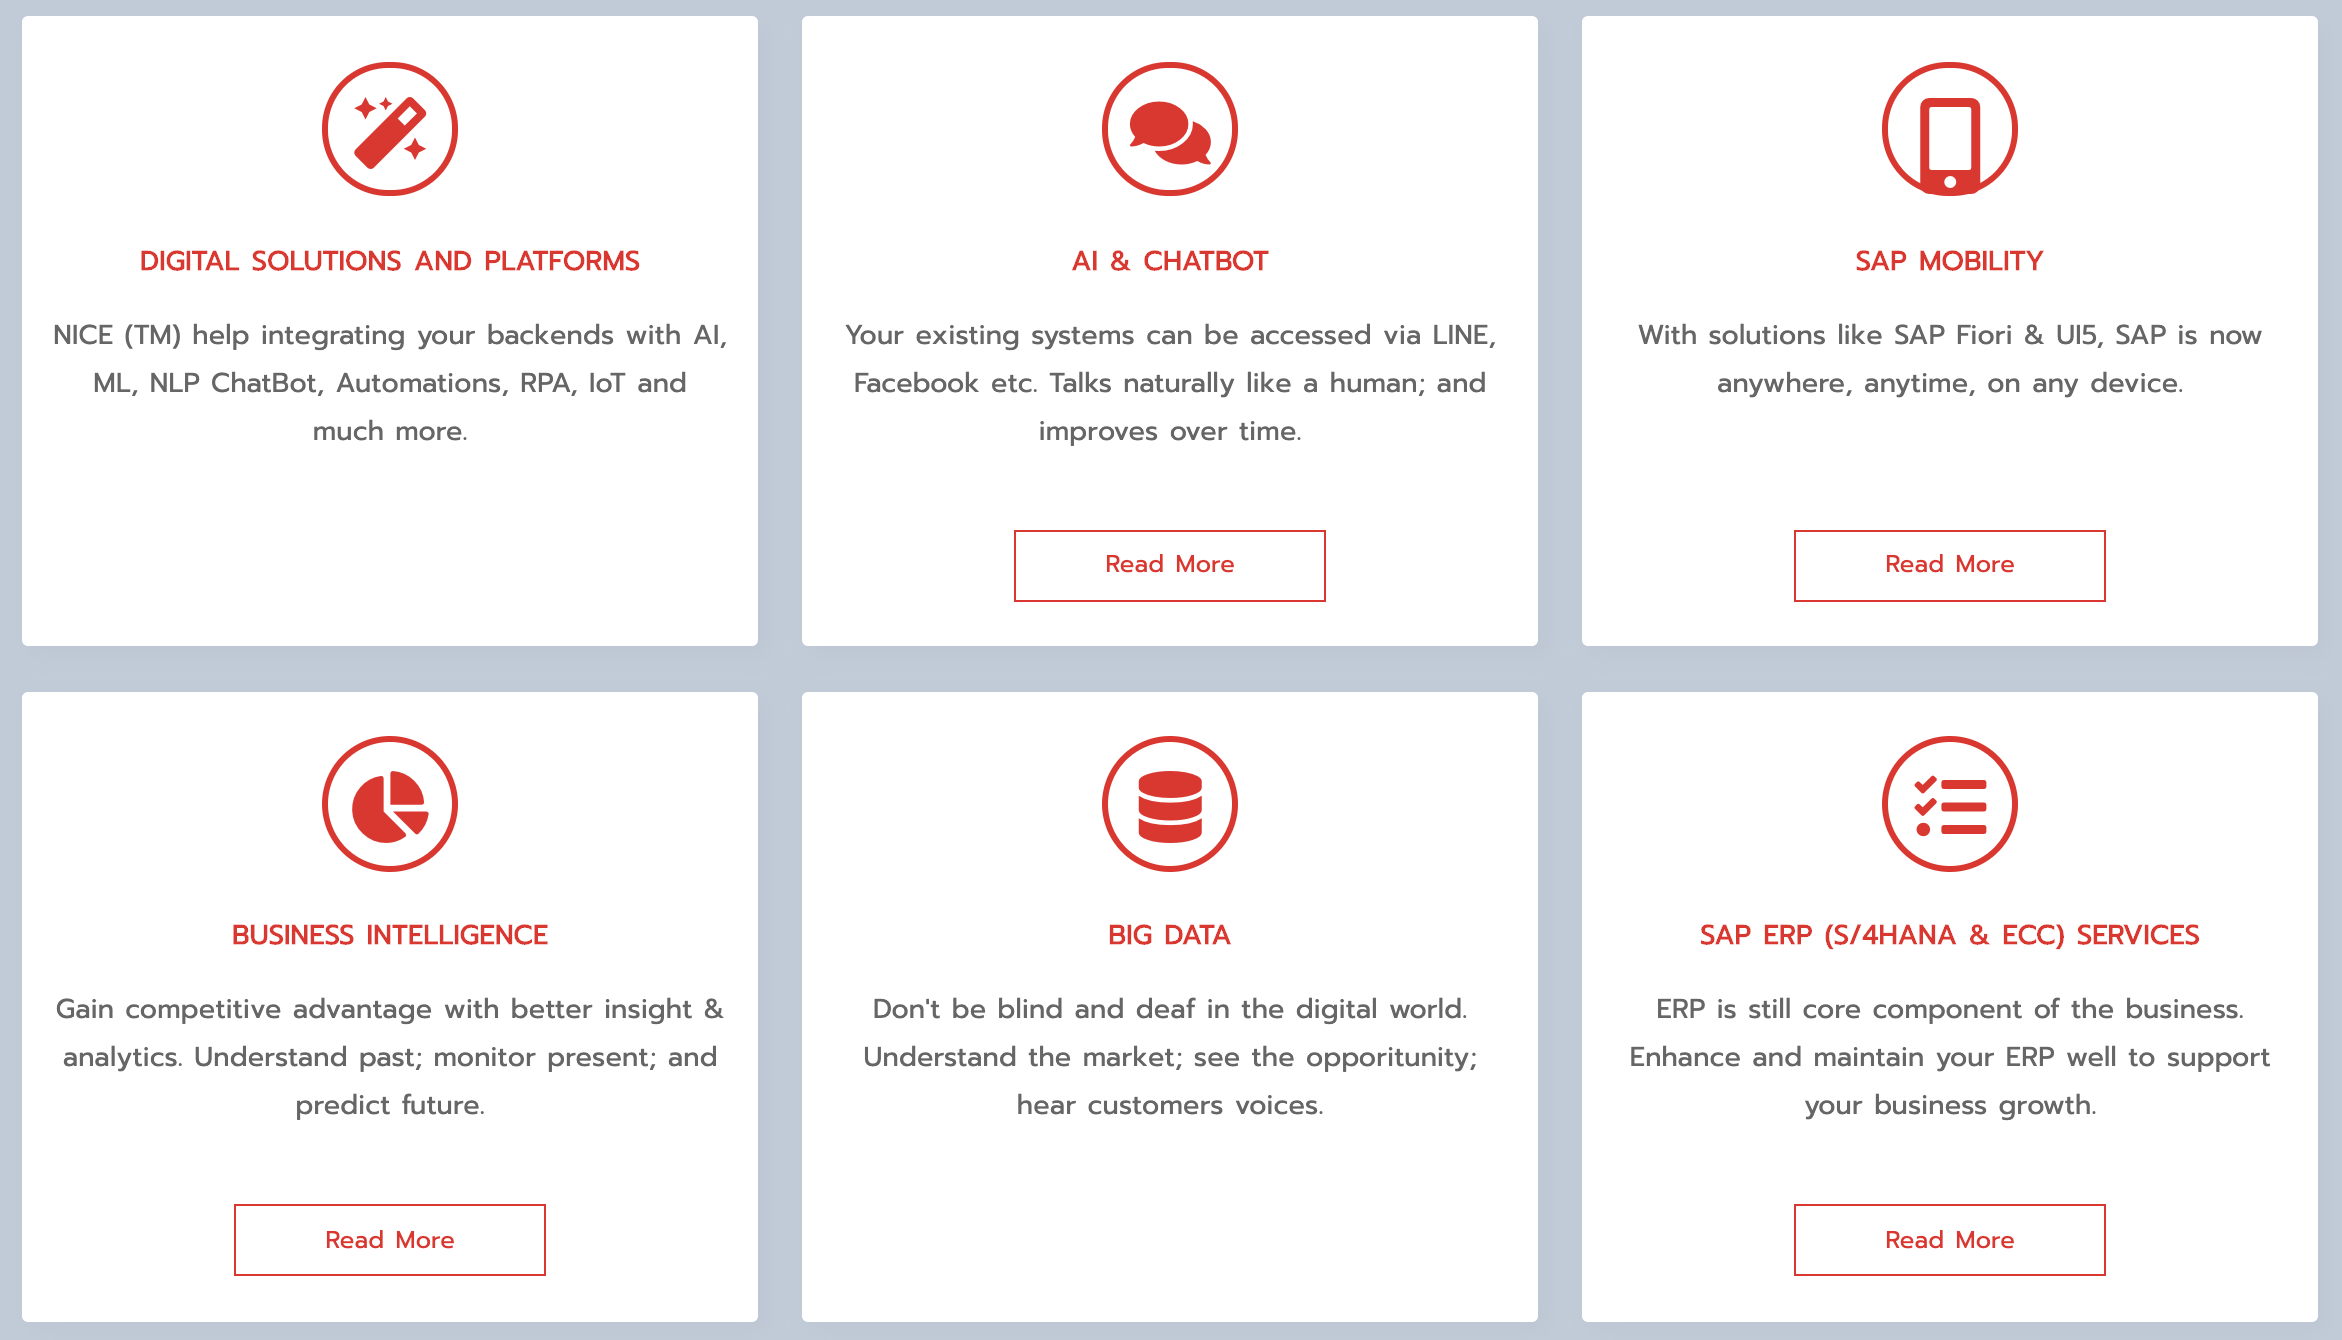
\includegraphics[width=1\columnwidth]{zygen-services.png}
  \caption{ตัวอย่างการให้บริการของ บริษัท ไซเจ็น}
  \label{Fig:zygen-services}
\end{figure}

\subsection{ตำแหน่งและลักษณะงานที่นักศึกษาได้รับมอบหมายให้รับผิดชอบ}

ตำแหน่ง: Full Stack Developer

หน้าที่: พัฒนาเว็บแอพพลิเคชั่นตามความต้องการของลูกค้า

\subsection{ชื่อและตำแหน่งของพนักงานที่ปรึกษา}

ชื่อ-นามสกุล: นายวิวัฒน์ เส็งอนันต์

ตำแหน่ง: Web Developer

แผนก: Development Team

\subsection{ระยะเวลาปฏิบัติงาน}

ช่วงเวลาปฏิบัติงาน: 1 มิถุนายน 2563 - 30 กันยายน 2563

ช่วงเวลาปฏิบัติงาน: จันทร์ - ศุกร์ เวลา 09:00 น. - 18:00 น.

รวมระยะเวลา: 4 เดือน



    \chapter{รายละเอียดการปฏิบัติงาน}
\label{chapter:related-theory}

\section{ตำแหน่งและลักษณะงานที่นักศึกษาได้รับมอบหมาย}

ตำแหน่ง: Full Stack Developer

\subsection{งานที่ได้รับผิดชอบ}

\begin{enumerate}
  \item ศึกษาเทคโนโลยีที่มีคุณภาพเพื่อประยุกต์ใช้กับการทำงาน
  \item พัฒนาเว็บแอพพลิเคชั่นประเมินความสามารถเบื้องต้นของผู้สมัครงาน
  \item ควบคุมคุณภาพของโค้ดให้มีคุณภาพที่ดี
\end{enumerate}

\section{รายละเอียดของโครงการที่ได้รับผิดชอบ}

เนื่องจากนักศึกษาได้รับหน้าที่ในตำแหน่ง Developer ในทีม BUDDY RECRUIT ซิ่งทำเกี่ยวกับการช่วยให้บริษัทหาคนเข้ามาทำงาน ได้ตรงตามความต้องการของบริษัท จึงได้รับมอบหมายให้ทำเว็บแอพพลิเคชั่นประเมินความสามารถเบื้องต้นของผู้สมัครงาน โดยเว็บแอพพลิเคชั่นนี้ช่วยให้คัดกรองผู้คนได้มีประสิทธิภาพมากยื่งขึ้น ผ่านการทำข้อสอบที่สามารถกำหนดระดับความยากของข้อสอบได้ และดึงคลังคำถามมาแบบสุ่ม ส่งให้ผู้ทำข้อสอบโดยอัติโนมัติผ่านทางอีเมล เมื่อผู้สมัครงานทำข้อสอบเสร็จแล้ว ข้อสอบจะถูกส่งไปที่ผู้ออกข้อสอบ พร้อมตรวจข้อที่เป็นคำถามปรนัยให้อัตโนมัติ โดยระบบนี้แบ่งเป็น 2 ส่วนหลักๆ ได้แก่

\begin{enumerate}
  \item ส่วนต่อประสานกับผู้ใช้(Front-end) เป็นส่วนที่ผู้ใช้งานสามารถมีปฏิสัมพันธ์กับเว็บแอพพลิเคชั่นได้ ผ่าน UI(User Interface) ที่หน้าเว็บแอปพลิเคชั่น
  \item ส่วนที่จัดการกับฐานข้อมูล(Back-end) เป็นส่วนที่ผู้ใช้งานไม่สามารถมองเห็นได้จากภายนอก เป็นการทำงานหลักๆของเว็บแอพพลิเคชั่น เช่น การเก็บข้อมูล การเรียกใช้ข้อมูล และการเชื่อมต่อการทำงานร่วมกับระบบอื่นๆ
\end{enumerate}

อนึ่ง ข้อมูลข้างต้นเป็นเพียงภาพรวมของเว็บแอพพลิเคชั่นโดยย่อ ซึ่งรายละเอียดของเว็บแอพพลิเคชั่นนี้จะกล่าวโดยละเอียดในบทถัดไป

\section{แนวคิดและทฤษฏีที่เกี่ยวข้อง}

\subsection{RESTful Web Services (RWS)}

เป็น web service ที่ใช้ REST architectural style โดยจะอนุญาติให้ระบบ Request และเข้าถึง Resource บนเว็บโดยใช้ชุดคำสั่งที่กำหนดเอาไว้  การตอบโต้ของ REST อยู่บนพื้นฐานของ Hypertext Transfer Protocol (HTTP) โดย Request จะส่งคำขอไปยัง URI ที่กำหนด และส่งข้อมูลกลับมาในรูปแบบ HTML, XML, JSON หรือ format อื่นๆ ทำให้สามารถบำรุงรักษาง่าย และสามารถ scale service ได้~\cite{Guru99}

\begin{itemize}
  \item Client-server architecture: Client ผู้ที่เข้ามาขอ resources ไม่ต้องรู้ Business logic ภายใน ส่วน Server มีหน้าที่เก็บข้อมูล ไม่จำเป็นต้องรู้เกี่ยวกับ UI หรือสถานะของผู้เรียก
  \item Stateless: ส่ง request ให้เซิร์ฟเวอร์แล้วรับกลับมาเป็น response เมื่อรับ response มาแล้วจบการทำงาน
  \item Cache: สามารถกำหนดได้ว่าจะเก็บ cache ของ response นั้นหรือไม่
  \item Layered system: สามารถปรับปรุงความสามารถในการขยายระบบได้ โดยการใช้งานการทำ Load balance
  \item Interface/Uniform Contract: วิธีการที่จะคุยกับเซิร์ฟเวอร์โดยไม่คำนึงถึงประเภทของอุปกรณ์ หรือประเภทของแอพพลิเคชั่น
\end{itemize}

\subsection{HTTP Request}

HTTP คือ protocol ที่อนุญาติให้ไคลเอนต์ดึงข้อมูลจากเซิร์ฟเวอร์~\cite{Guru99}

\begin{itemize}
  \item Request-Line คือส่วนที่ระบุ HTTP Method, Request-URI และ version ของ protocol เช่น HTTP/1.0, HTTP/1.1, HTTP/2.0
  \item Headers คือส่วนที่อนุญาติให้ใส่ข้อมูลเพิ่มเติม หรือกฏเกณฑ์ต่างๆเกี่ยวกับการ request เช่น รูปแบบของข้อมูล, การเข้ารหัส
  \item Body คือส่วนที่ระบุข้อมูลที่ต้องการจะส่งให้ปลายทาง สามารถส่ง patameter ต่างๆ ไปใน Body เพื่อเพิ่ม, ลบ หรือแก้ไขข้อมูลบนเซิร์ฟเวอร์ได้
\end{itemize}

\subsection{HTTP Request Methods}

คือส่วนที่ใช้ในการกำหนดประเภทของคำร้องขอต่างๆ บน HTTP Request~\cite{Guru99} โดยมี 4 Methods หลักคือ 

\begin{itemize}
  \item POST สำหรับใช้เพื่อสร้างค่าใหม่ เช่น สร้างรายชื่อพนักงานใหม่
  \item GET สำหรับขอข้อมูลจากเซิร์ฟเวอร์ เช่น ขอข้อมูลพนักงานทั้งหมด
  \item PUT สำหรับแก้ไขค่าต่างๆบนเซิร์ฟเวอร์ โดยส่งมาใน body ของ HTTP Request เช่น แก้ไขข้อมูลของพนักงาน
  \item DELETE สำหรับลบค่าบนเซิร์ฟเวอร์ เช่น ลบข้อมูลของพนักงาน
\end{itemize}

\subsection{HTTP Response Status Code}

คือมาตรฐานสถานะที่เซิร์ฟเวอร์ตอบสนองกับเว็บไซต์ต่างๆ~\cite{httpResponse}

\begin{itemize}
  \item 2xx (Successful) 
  
  Request ที่ไคลเอนต์ส่งไปยังเซิร์ฟเวอร์ถูกประมวลผลเรียบร้อย และไม่มี error ใดๆ ประกอบด้วย

  200 : (OK) ส่ง request สำเร็จ

  201 : (Created) ผู้ใช้สร้างข้อมูลลง database สำเร็จ response นี่จะได้รับหลัง POST หรือ PUT requests

  202 : (Accepted) request สำเร็จแล้วแต่ เซิร์ฟเวอร์ยังประมวลผลไม่เสร็จ
  
  203 : (Non-Authoritative Information) เซิร์ฟเวอร์ประมวลผลสำเร็จแล้ว แต่ทำการส่งข้อมูลมาจากแหล่งอื่น

  204 : (No Content) เซิร์ฟเวอร์ประมวลสำเร็จแล้ว แต่ไม่มีข้อมูลที่ต้องส่งคืนไป

  206 : (Partial Content) เซิร์ฟเวอร์ส่งข้อมูลบางส่วน ตามที่คลเอนต์ต้องการ โดยกำหนดขอบเขตที่ต้องการผ่าน headers บน HTTP Request

  \item 3xx (Redirection)
  
  request ที่ไคลเอนต์ส่งไปหาเซิร์ฟเวอร์ แล้วถูก redirect ส่งไปประมวลผลที่อื่น เพื่อทำให้กระบวน \\ การทำงานสำเร็จ

  300 : (Multiple Choices) request ที่ไคลเอนต์ส่งไปมี response มากกว่า 1 ตัว ไคลเอนต์สามารถเลือกลิงค์ที่จะ redirect ไปได้

  301 : (Moved Permanently) URL ที่ทำการ request ขอข้อมูลถูกดปลี่ยนไปถาวร จึง response ออกมาเป็น URL ใหม่

  302 : (Found) URL ที่ทำการ request มีการเปลี่ยนชั่วคราว

  303 : (See Other) request ที่เรียกอยู่ภายใต้ URL อื่น

  304 : (Not Modified) response นี้ยังไม่ถูกแก้ไข ดังนั้น ไคลเอนต์จะได้รับ response ที่เป็น cached version

  \item 4XX (Client Error)
  
  เกิด error มาจาก request ของไคลเอนต์ที่ผิดพลาด เช่น ผิด URL หรือผิด syntax

  400 : (Bad Request) ไคลเอนต์เขียน syntax ผิด หรือ ไม่ถูกรูปแบบ ทำให้เซิร์ฟเวอร์ไม่เข้าใจ

  401 : (Unauthorized) ไคลเอนต์ต้องทำการยืนยันตัวตนก่อนที่จะได้รับ response

  403 : (Forbidden) ไคลเอนต์ทำการยืนยังตัวตนแล้ว แต่ไม่มีสิทธิ์ในการเข้าถึงข้อมูลนี้

  404 : (Not Found) ถ้าเกิดบน browser คือ URL ไม่ถูกจดจำบนเซิร์ฟเวอร์ แต่ถ้าเกิดบน API  คือ มีการขอข้อมูลที่ถูกต้อง แต่ไม่มีข้อมูลนี้อยู่

  405 : (Method Not Allowed) method ที่เรียกใช้ไม่ถูกต้อง

  406 : (Not Acceptable) header ที่ไคลเอนต์ request ไม่สัมพันธ์กับเซิร์ฟเวอร์

  413 : (Payload Too Large) request ที่ขอใหญ่กว่า limit ที่เซิร์ฟเวอร์กำหนดไว้

  414 : (URI Too Long) URL ที่ทำการ request โดยไคลเอนต์ ยาวกว่าที่เซิร์ฟเวอร์จะยอมรับได้

  415 : (Unsupported Media Type) เซิร์ฟเวอร์ไม่รองรับ media (รูป หรือ สื่อต่างๆ) ดังนั้นเซิร์ฟเวอร์จึงปฏิเสธการ request

  \item  5XX (Server Error)
  
  เซิร์ฟเวอร์มีปัญหา

  500 : (Internal Server Error) เซิร์ฟเวอร์เจอกับสถานการณ์ที่ไม่สามารถจัดการได้

  501 : (Not Implemented) ไคลเอนต์เรียก request method ที่เซิร์ฟเวอร์ไม่รองรับ และเซิร์ฟเวอร์ไม่สามารถจัดการได้

  502 : (Bad Gateway) เซิร์ฟเวอร์เป็น gateway หรือ proxy ได้รับ response ที่ผิดพลาดจากเซิร์ฟเวอร์อื่น

  503 : (Service Unavailable) เซิร์ฟเวอร์อยู่ระหว่างการปรับปรุง หรือยังไม่พร้อมที่จะจัดการ request

  504 : (Gateway Timeout) เซิร์ฟเวอร์เป็น gateway และไม่สามารถ response ข้อมูลในเวลาที่กำหนดได้

\end{itemize}

\subsection{MVC (Model View Controller)}

คือ software design pattern ที่แยกการทำงานขอโปรแกรมออกเป็น 3 ส่วนเพื่อแยกข้อมูลภายในโปรแกรมกับข้อมูลที่แสดงให้ผู้ใช้เห็น~\cite{mvc}

\begin{itemize}
  \item Model คือส่วนที่เป็นโครงสร้างของข้อมูล กำหนดกฎเกณฑ์ของการเก็บข้อมูล และเป็นส่วนที่ไว้สำหรับการจัดการข้อมูลโดยตรง
  \item View คือส่วนที่ไว้แสดงผลตามที่ผู้ใช้ต้องการ ผู้ใช้สามารถเปลี่ยนแปลงข้อมูลที่ผู้ใช้เห็นได้
  \item Controller คือส่วนที่ไว้จัดการกับ Model โดยขึ้นอยู่กับการกระทำของ View ที่กำหนดโดยผู้ใช้ และสรรหาข้อมูลจาก Model เพื่อไปแสดงใน View
\end{itemize}

\begin{figure}[H]
  \centering
  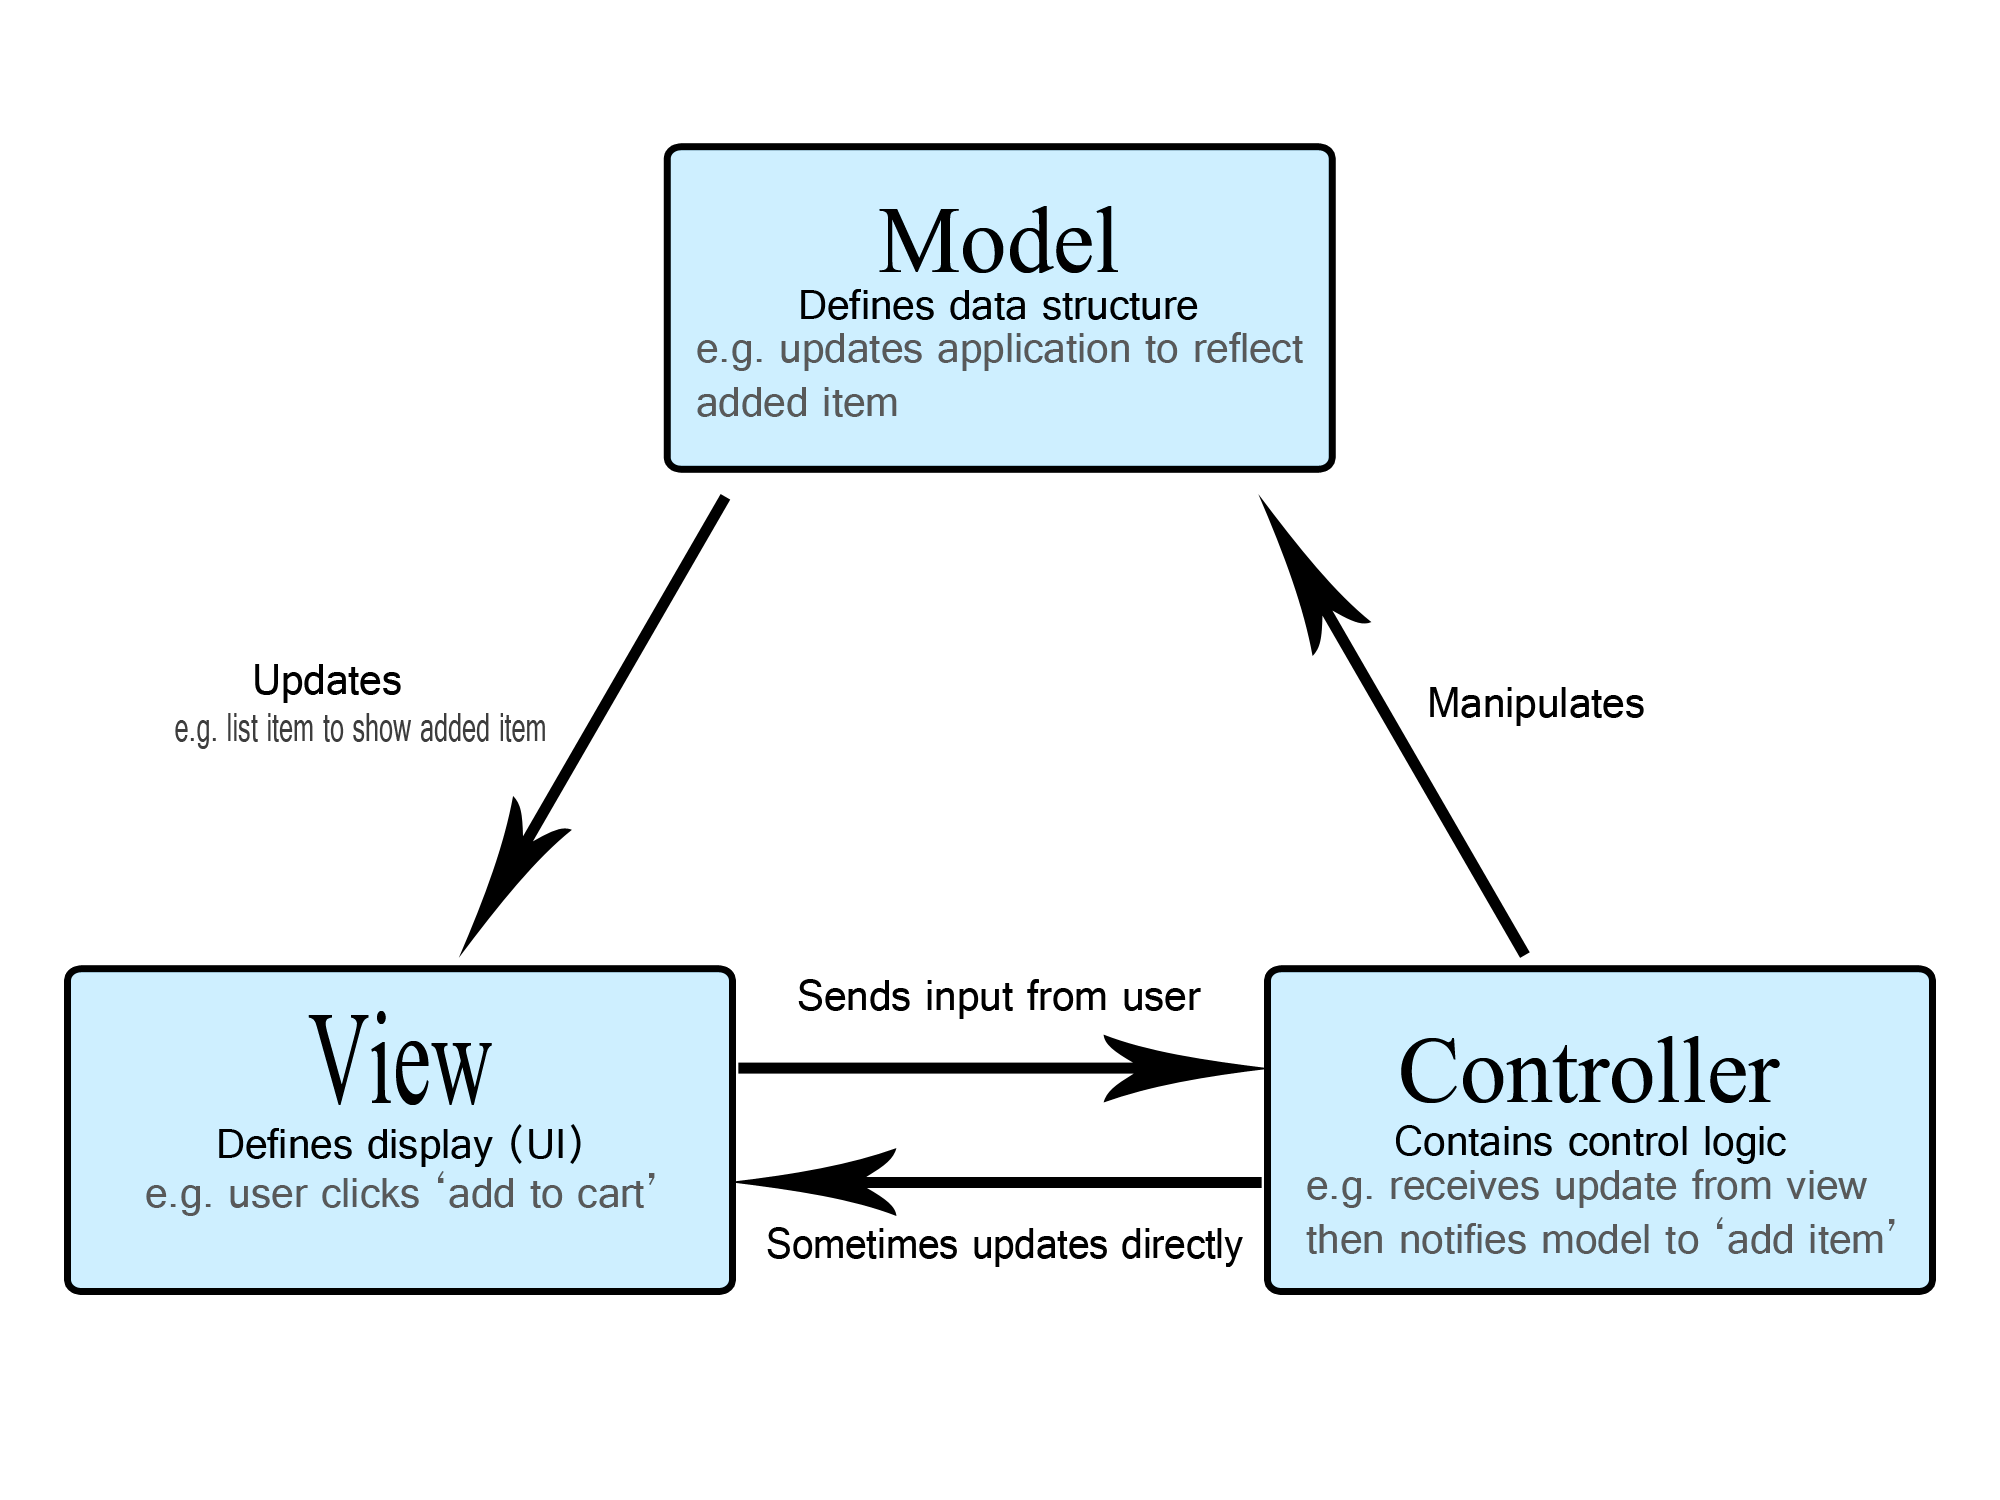
\includegraphics[width=0.8\columnwidth]{model-view-controller.png}
  \caption{แสดง MVC architecture}
  \label{Fig:model-view-controller}
\end{figure}

\subsection{NoSQL Database}

คือ ฐานข้อมูลที่สร้างมาเพื่อให้จัดการข้อมูลที่มีความซับซ้อนได้ง่ายขึ้นเมื่อเทียบกับ SQL databases ที่มีการเก็บข้อมูลในที่รูปแบบแน่นอน (structured data) โดยเพิ่มความสามารถในการจัดเก็บข้อมูลในรูปแบบที่ไม่แน่นอน (unstructured data)  ทำให้สามารถเก็บข้อมูลที่ซับซ้อนได้, เพิ่มความสามารถในการขยายระบบในรูปแบบแนวนอน (Horizontal Scalability) เพื่อรองรับปริมาณข้อมูลในปัจจุบัน~\cite{nosql}
\begin{figure}[H]
  \centering
  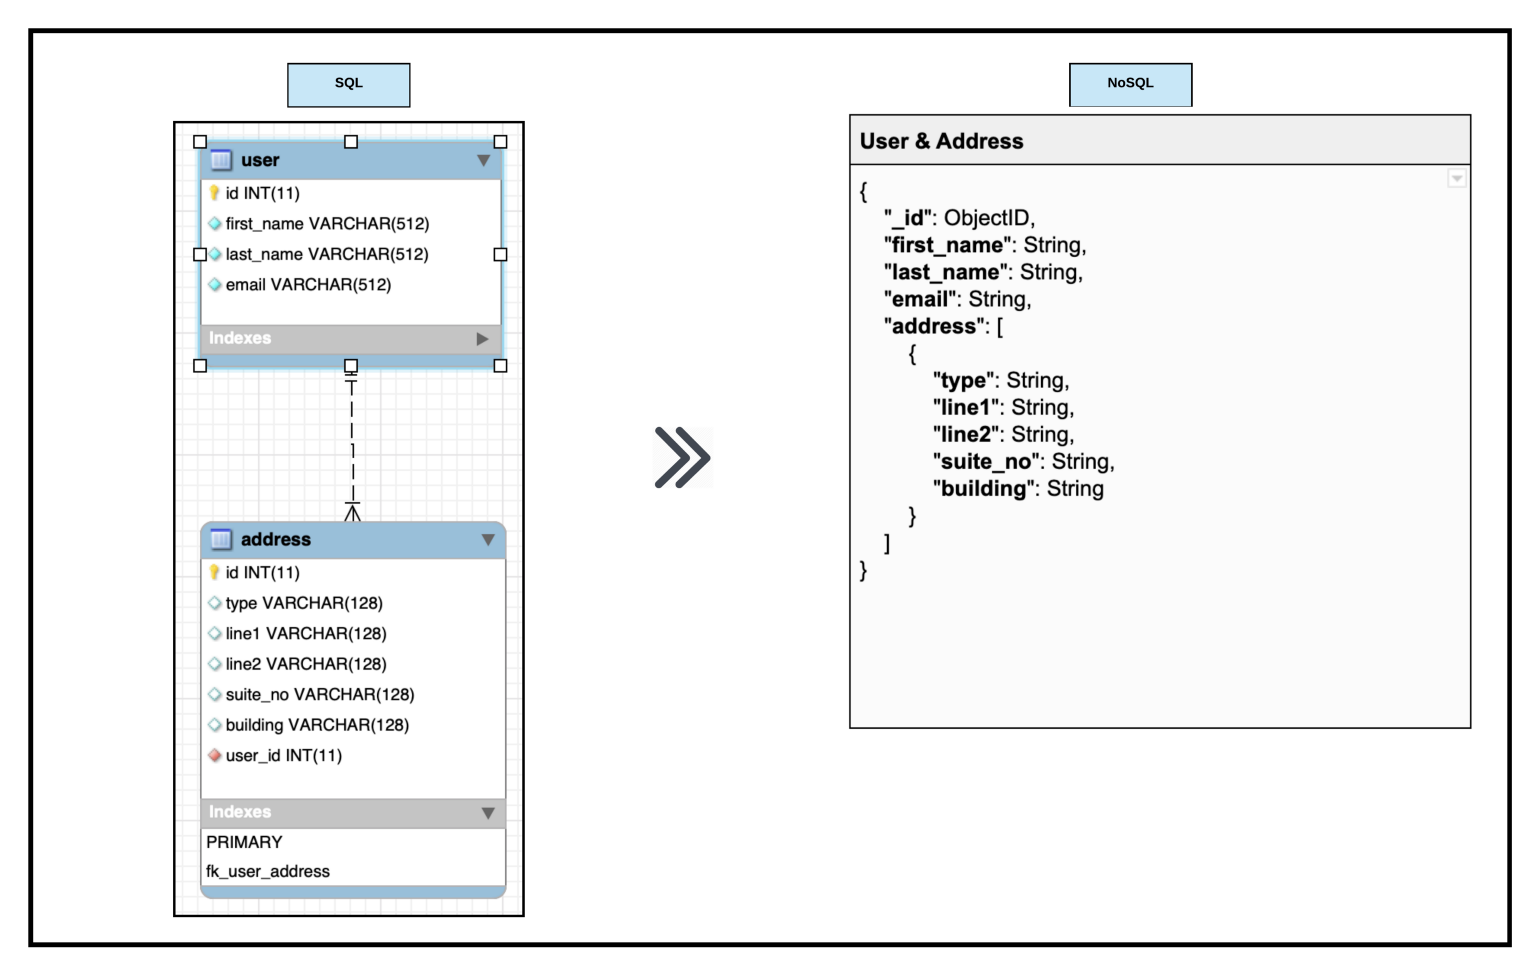
\includegraphics[width=0.9\columnwidth]{no-sql.png}
  \caption{แสดงตาราง SQL เปรียบเทียบกับตาราง NoSQL}
  \label{Fig:no-sql}
\end{figure}

\subsection{Token}

เป็นชุดรหัสเอาไว้ระบุตัวตนของผู้ใช้ว่าผู้ใช้นั้นเป็นใคร ไม่มีรูปแบบที่ตายตัว

\subsection{Container}

เป็นหน่วยของซอฟแวร์ที่ทำการลงทรัพยากรณ์ทุกอย่างที่ต้องใช้ในแอพ และตัวโค้ดของแอพ ดังนั้นแอพพลีเคชั้นจะสามารถถูกเรียกใช้ได้อย่างรวดเร็ว และใช้ในสภาพแวดล้อมใดก็สามารถทำงานได้ โดยมีความเป็นมาตรฐาน และประหยัดทรัพยากรที่ใช้ทำงานตัวแอพพลีเคชั่น~\cite{container}

\subsection{Model–view–viewmodel}

เป็น software architectural pattern รูปแบบที่ช่วยแยกการพัฒนาแอพพลีเคชั่นออกเป็น 3 ส่วน โดยแบ่งออกจากกันอย่างชัดเจนเพื่อให้ง่ายต่อการจัดการและแสดงกระบวนการทำงานในแต่ละส่วน~\cite{mvvm}

\begin{itemize}
  \item Model คือส่วนที่เป็นโครงสร้างของข้อมูล กำหนดกฎเกณฑ์ของการเก็บข้อมูล  และเป็นส่วนที่ไว้สำหรับการจัดการข้อมูลโดยตรง
  \item View คือส่วนที่ไว้แสดงผลตามที่ผู้ใช้ต้องการ ผู้ใช้สามารถเปลี่ยนแปลงข้อมูลได้
  \item View model มีหน้าที่เก็บข้อมูลทั้งหมดที่ View ต้องการ โดย View และ View model มีการใช้ Data-binding ซึ่งกันและกัน กล่าวคือถ้าข้อมูลของ View มีการแก้ไข ข้อมูลของ View model จะได้รับการแก้ไขไปด้วย หรือข้อมูลของ View model มีการแก้ไข ข้อมูลของ View จะได้รับการแก้ไขไปด้วย
\end{itemize}

\begin{figure}[H]
  \centering
  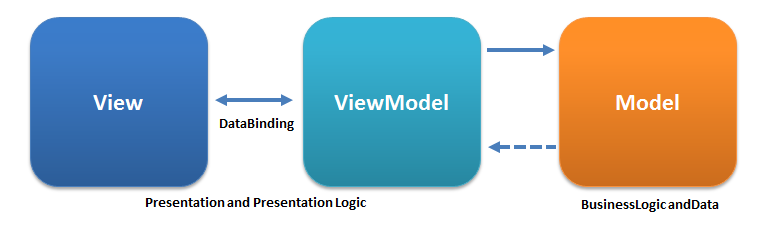
\includegraphics[width=0.9\columnwidth]{MVVMPattern.png}
  \caption{แสดง MVVM architecture}
  \label{Fig:MVVMPattern}
\end{figure}

\newpage

\section{เครื่องมือและเทคโนโลยีที่ใช้ในการปฏิบัติงาน}

\subsection{Trello}

เป็นเว็บแอพพลิเคชั่นที่ช่วยจัดการบริหารโปรเจ็กต์ ให้เป็นระเบียบได้อย่างเรียบง่ายเปรียบเสมือนกระดานไว้วางแผนการทำงาน ระบุรายละเอียดของงานแต่ละงาน โดยเว็บแอพพลิเคชั่นนี้สามารถใช้งานร่วมกันภายในทีมได้ ทำให้การทำงานต่างๆในโปรเจ็กต์มีความคล่องตัวมากยิ่งขึ้น

\begin{figure}[H]
  \centering
  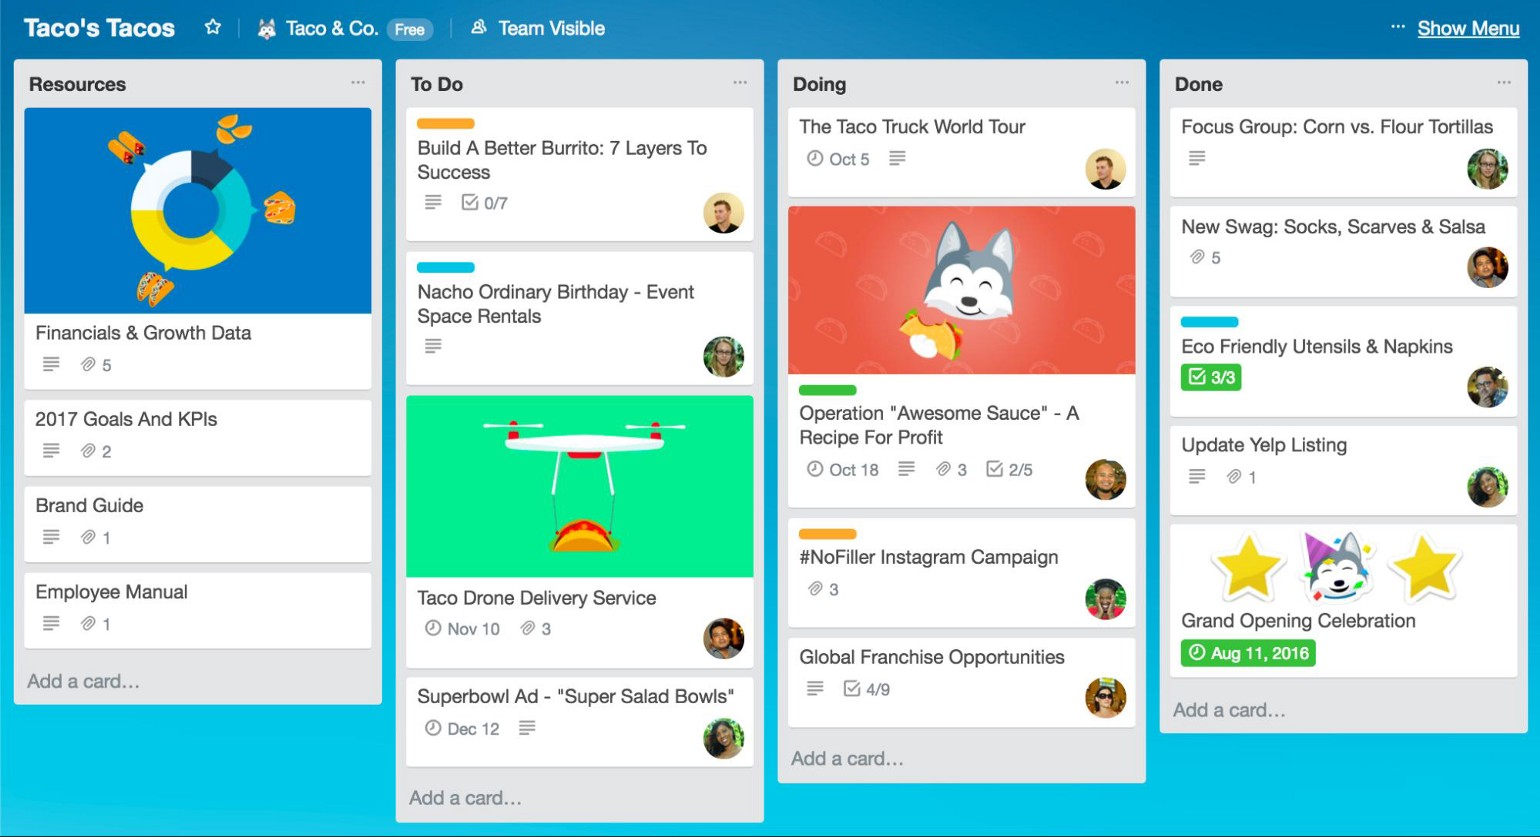
\includegraphics[width=0.9\columnwidth]{trello.png}
  \caption{แสดงตัวอย่างการใช้งาน Trello}
  \label{Fig:trello}
\end{figure}

\subsection{Figma}

เป็นเครื่องมือที่นำมาใช้ในการออกแบบ prototype ของงานที่ทำ โดยสามารถใช้งานแอพพลิเคชั่น Figma ได้ในทุกแพลตฟอร์ม

\begin{figure}[H]
  \centering
  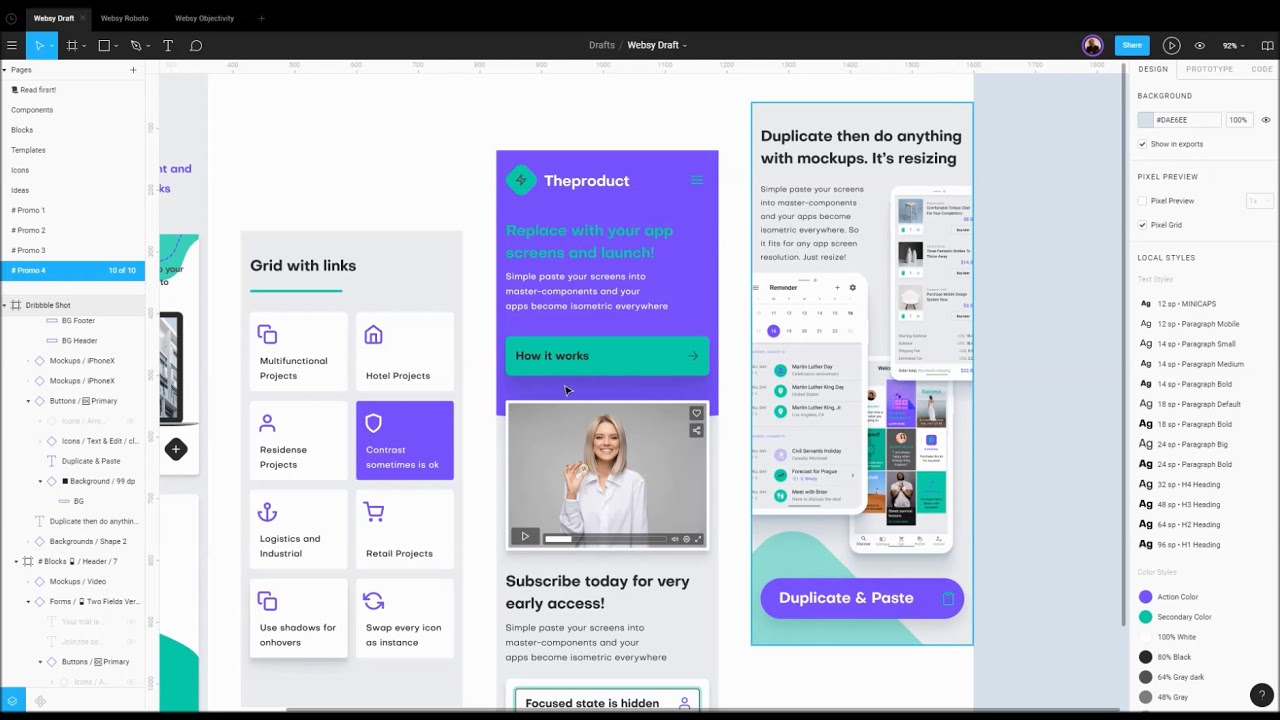
\includegraphics[width=0.9\columnwidth]{figma.jpg}
  \caption{แสดงตัวอย่างการใช้งาน Figma}
  \label{Fig:figma}
\end{figure}

\subsection{Visual Studio Code}

เป็นโปรแกรม code editor ที่ใช้ในการเขียน แก้ไข และปรับแต่งโค้ด โดยพัฒนาออกมาในรูปแบบ OpenSource โดยมีความสามารถในการเปลี่ยนสี Syntax ของโค้ด ตามแต่ละภาษา เพื่อให้ง่ายต้อการมองและการขียนโค้ด ซึ่งสนับสนุนภาษามากมาย ยกตัวอย่างเช่น ภาษา C++, Java, JavaScript, PHP, Python เป็นต้น และยังสามารถติดตั้งส่วนขยายที่เพิ่มความสะดวกสบายในการเขียนโค้ด ตามที่เราต้องการได้

\begin{figure}[H]
  \centering
  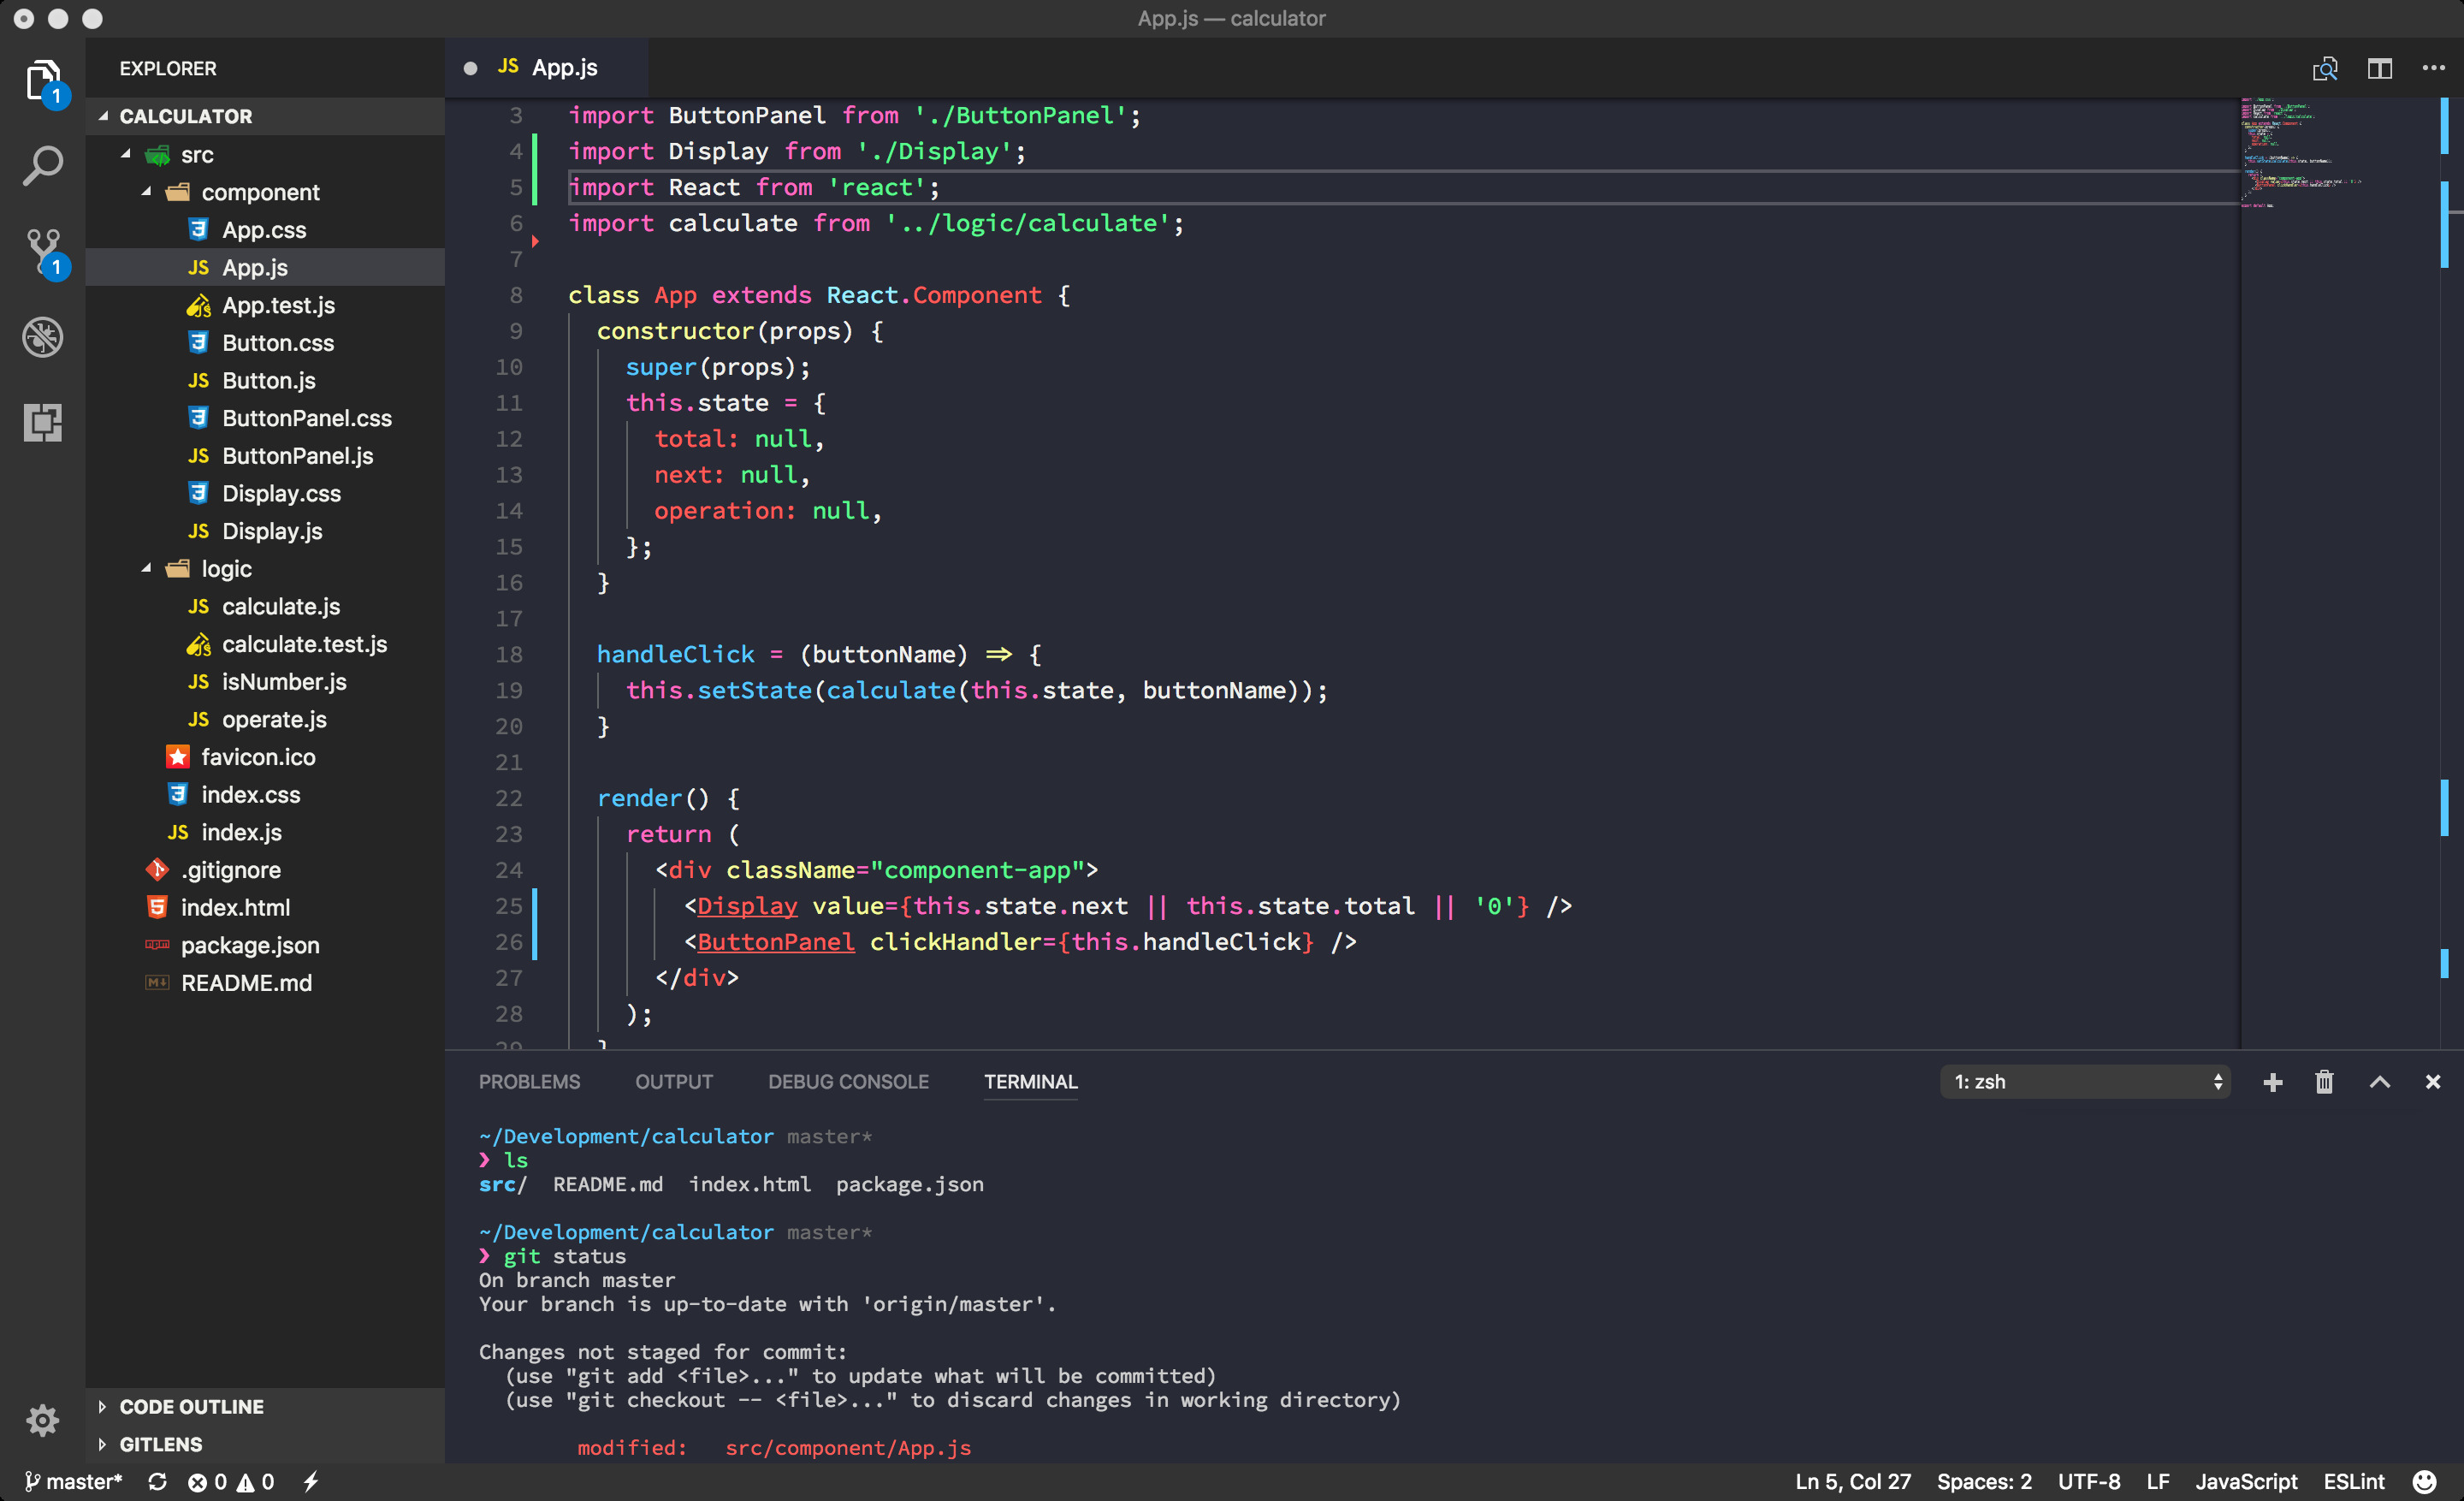
\includegraphics[width=0.9\columnwidth]{vscode.jpg}
  \caption{แสดงตัวอย่างการใช้งาน vscode}
  \label{Fig:vscode}
\end{figure}

\subsection{Vue.js}

เป็น JavaScript Framework ที่สร้างส่วนต่อประสานกับผู้ใช้ (UI) และเป็น single-page applications คือ wep application ที่ทำการโหลด page เพียงครั้งเดียวแต่สามารถเรียกข้อมูลอื่นๆแบบ dynamic ได้ ทำให้ประสบการณ์การใช้งานเว็บใกล้เคียง native app มากยิ่งขึ้น

\subsection{VueX}

เป็น state management pattern ที่ผสมผสานกับ library เพื่อใช้สำหรับจัดการ state เพื่อให้ data flow ของโปรเจคไปในทิศทางเดียวกัน code จึงมีความเป็นระบบมากยิ่งขึ้น และลดการเขียน code ที่ซับซ้อน ทำให้การทำงานร่วมกันภายในทีมสะดวกมากยิ่งขึ้น เช่นการให้คนในทีมรับผิดชอบแต่ละ module~\cite{vuex}

\subsection{Node.js}

เป็น JavaScript runtime กล่าวคือเป็นตัวที่ทำให้ JavaScript  สามารถใช้งานในส่วนของ backend หรือเซิร์ฟเวอร์ได้

\subsection{Express.js}

เป็น Node.js web application framework  ซึ่งมีฟิจเจอร์ต่างๆที่ช่วยให้พัฒนาเซิร์ฟเวอร์ด้วย Node.js ได้สะดวกมากยิ่งขึ้น เช่นการจัดการ request และ response

\subsection{Git}

เป็น Version control ที่เอาไว้ติดตาม และควบการเปลี่ยนแปลงของโค้ดเพื่อให้นักพัฒนา สามารถทำงานร่วมกันได้อย่างมีประสิทธิภาพ~\cite{git}

\subsection{Github}

เป็น website Git (version control repository) สำหรับนักพัฒนาซอฟแวร์ ใช้หลักการทำงานของ git แต่สามารถใช้งานร่วมกับผู้อื่นได้ผ่านอินเตอร์เน็ต

\subsection{Docker}

เป็น engine ที่มีการจำลองสภาพแวดล้อมขึ้นมาบนเครื่องเซิร์ฟเวอร์ เพื่อทำการนำ service ที่ต้องการมาทำงานอยู่บนเซิร์ฟเวอร์ โดยใช้หลักการ container ในการจำลองสภาพแวดล้อมขึ้นมาทำงาน service ของเราโดยที่ไม่ต้องมีการนำ os เข้ามาใช้ ทำให้ service ทำงานในสภาพแวดล้อมใดก็ได้~\cite{container}

\begin{figure}[H]
  \centering
  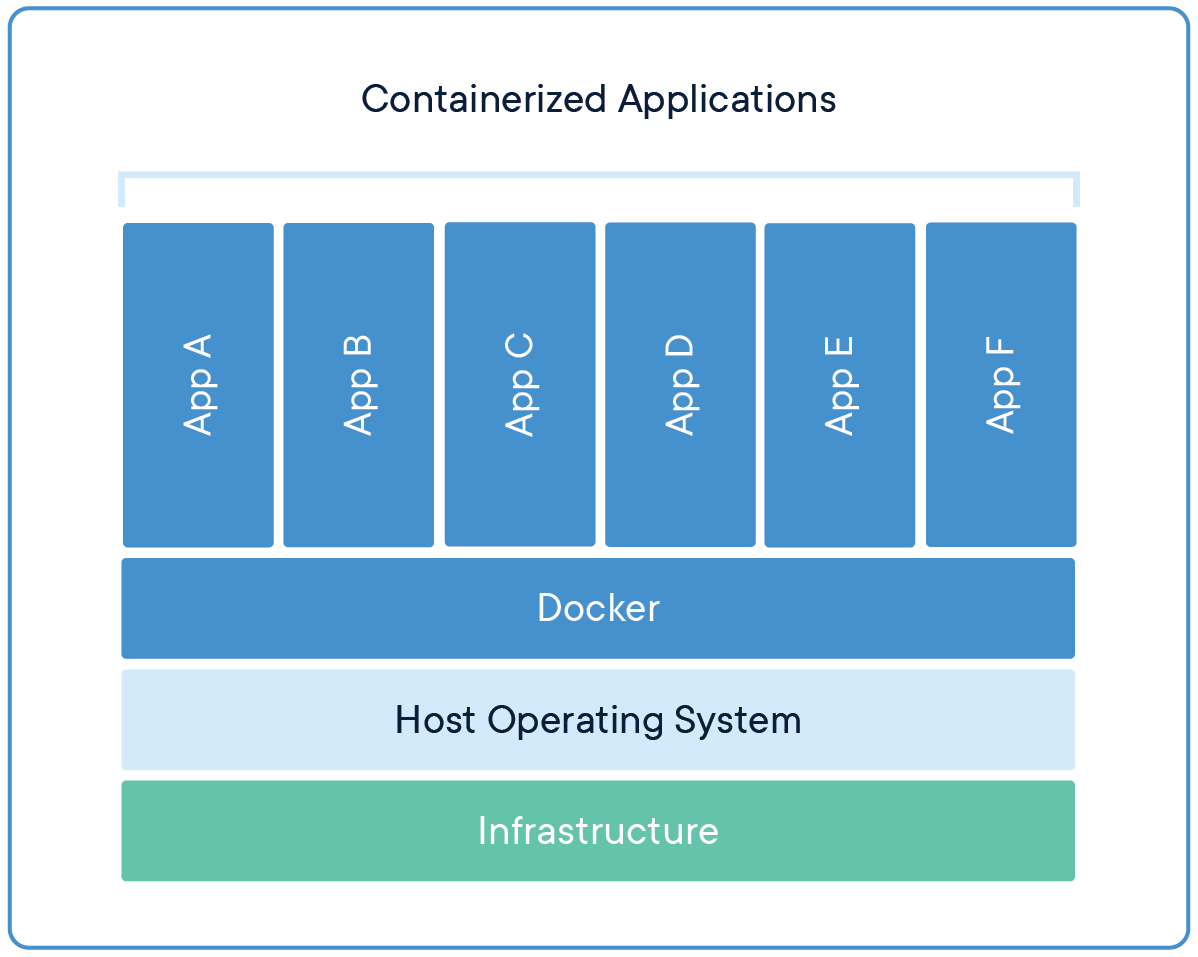
\includegraphics[width=0.8\columnwidth]{docker.png}
  \caption{แสดงตัวอย่างการทำงานของ docker}
  \label{Fig:docker}
\end{figure}

\subsection{Postman}

เป็นเครื่องมือที่มาช่วยในการ API เพิ่อทดสอบการทำงานของ Service โดยมีหน้าตาส่วนต่อประสานกับผู้ใช้(UI) ที่สวยและใช้งานง่าย

\begin{figure}[H]
  \centering
  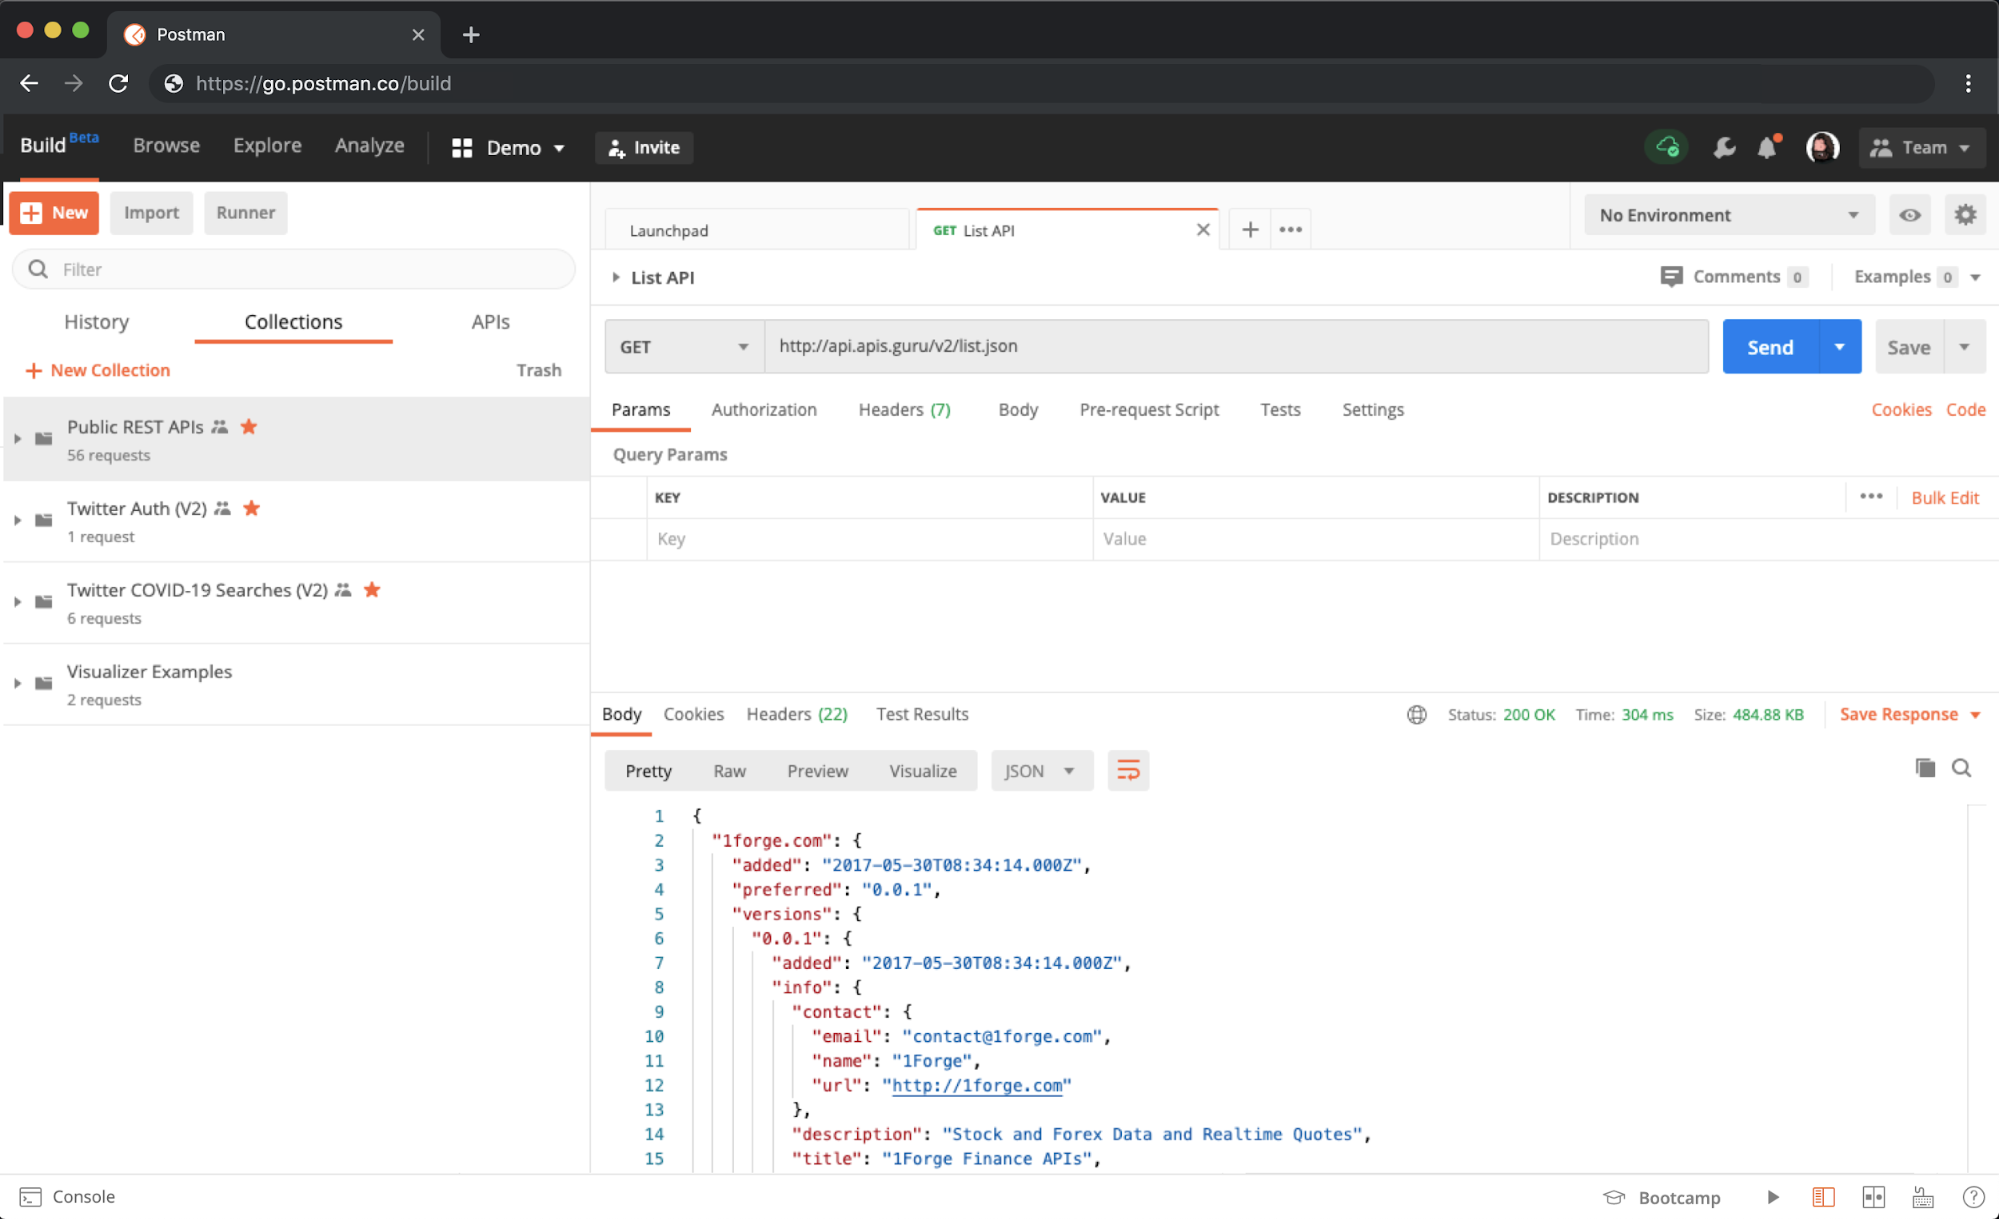
\includegraphics[width=0.9\columnwidth]{postman.png}
  \caption{แสดงตัวอย่างการใช้งาน postman}
  \label{Fig:postman}
\end{figure}

\subsection{JWT (Json Web Token)}

เป็นมาตรฐาน RFC 7519 ในการยืนยันตัวตน (Authentication) ที่เข้ามาแก้ปัญหาการส่งข้อมูลระหว่างกันในวิธีแบบดั้งเดิมคือ Server Based Authentication ที่เปลืองทรัพยากรในการเก็บ Session ID และไม่รองรับการขยายตัว (Scalability)  โดย JWT นั้นสามารถเก็บข้อมูลภายในตัวได้ และมีขนาดที่กระทัดรัด เพื่อนำมาใช้กับ Single Page Web Application (SPA)~\cite{jwt} โดย JWT แบ่งโครงสร้างออกเป็น 3 ส่วน

\begin{enumerate}
  \item Header เก็บประเภทของ token
  \item Payload เก็บข้อมูล
  \item Signature เป็นลายเซ็นที่อยู่ในรูปแบบของอิเล็กทรอนิกส์ (Digital Signed) เพื่อเช็คว่าเป็น token ที่ถูกสร้างอย่างถูกต้องหรือไม่  
\end{enumerate}

\begin{figure}[H]
  \centering
  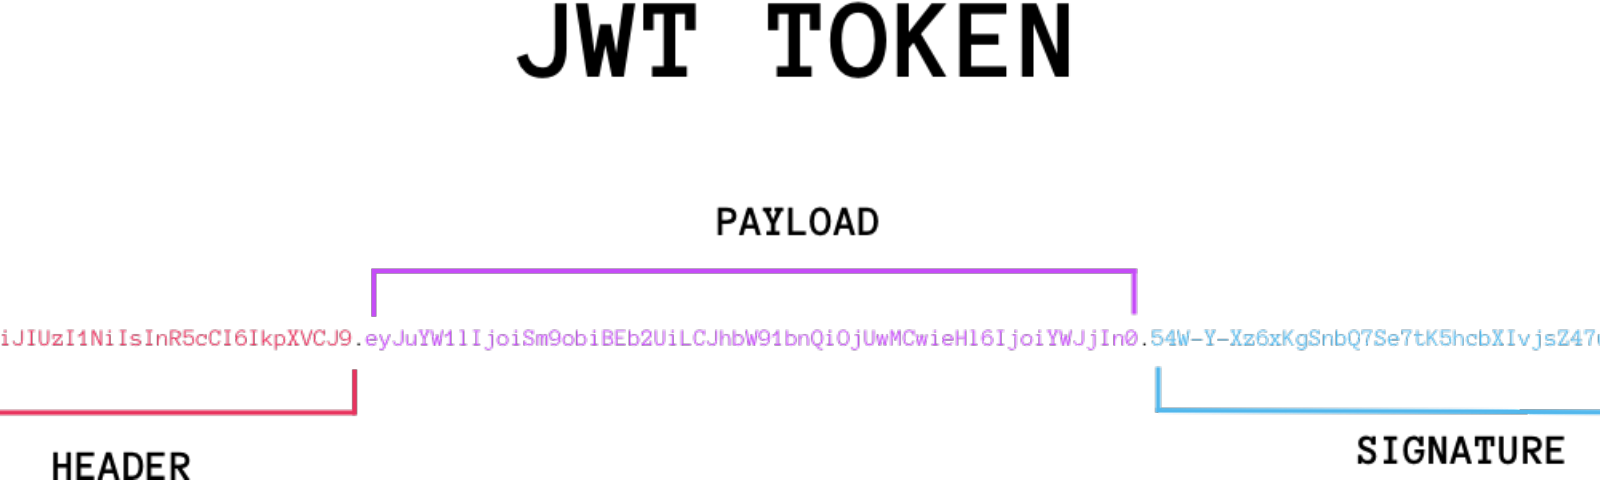
\includegraphics[width=0.9\columnwidth]{jwt.png}
  \caption{แสดงตัวอย่าง jwt endcoded}
  \label{Fig:jwt}
\end{figure}

\subsection{MongoDB}

เป็น open-source document database ประเภทหนึ่ง โดยเก็บข้อมูลแบบ NoSQL Database และเก็บข้อมูลในรูปแบบของ JSON (JavaScript Object Notation) ซึ่งเก็บเป็น key และ value ซึ่งมีสมรรถภาพสูงกว่าการเก็บด้วยโครงสร้างแบบแถวและหลัก(row/column) แบบดั้งเดิม~\cite{mongodb}

\subsection{Robo 3T}

เป็นการใช้ภาพเป็นตัวประสานกับผู้ใช้ของ(GUI) ของ MongoDB ช่วยทำให้ใช้งาน MongoDB ได้สะดวกมากยิ่งขึ้น เช่น เขียน SQL เพื่อ query ข้อมูลใน MongoDB หรือ Import และ export ไฟลล์ข้อมูลเป็น CSV, JSON, SQL and BSON/mongodump ได้~\cite{robo3t}

\begin{figure}[H]
  \centering
  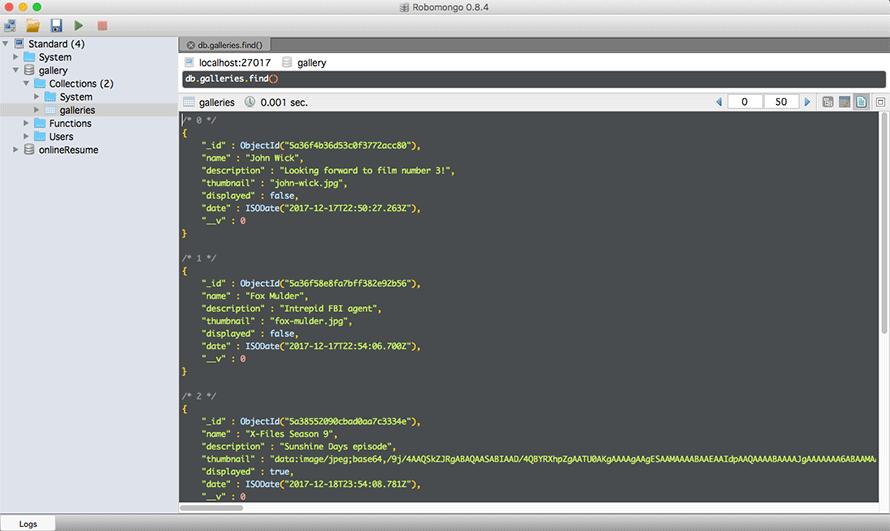
\includegraphics[width=0.9\columnwidth]{robo3t.png}
  \caption{แสดงตัวอย่างการใช้งาน Robo 3T}
  \label{Fig:robo3t}
\end{figure}

\subsection{SendGrid}

เป็น API ช่วยในการส่งอีเมลให้ผู้อื่น สามารถตรวจสอบอีเมลที่ส่งว่าส่งไปถึงหรือไม่ มีปัญหาอะไรเกินขึ้นหรือเปล่า และมีการเก็บสถิติข้อมูลอีเมลท่ีส่ง สรุปออกมาแสดงให้วิเคราะห์เช่น มีการเปิดเมลอ่านกี่ครั้ง มีการรายงานว่าเป็นสแปมกี่ครั้ง

\begin{figure}[H]
  \centering
  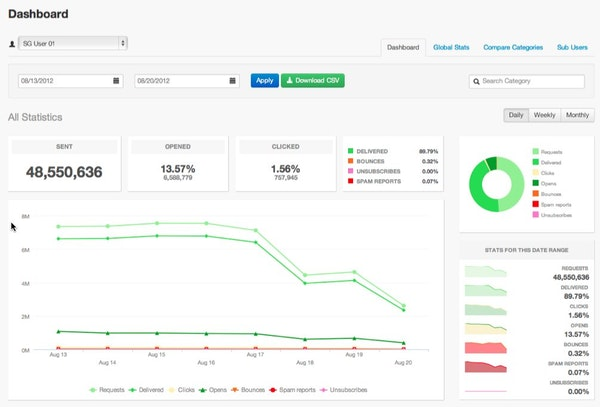
\includegraphics[width=0.9\columnwidth]{sendgrid.jpg}
  \caption{แสดงตัวอย่างสถิติของอีเมลที่ทำการส่งด้วย sendgrid}
  \label{Fig:robo3t}
\end{figure}

\section{ลักษณะขั้นตอนการทํางาน}


    \chapter{การออกแบบระบบและรายละเอียดการพัฒนา}
\label{chapter:experiment}

\section{ภาพรวมของเว็บแอพพลิเคชั่น}

เว็บแอพพลิเคชั่นประเมินความสามารถเบื้องต้นของผู้สมัครงาน คือระบบที่จะช่วยให้คัดกรองผู้คนได้มีประสิทธิภาพมากยื่งขึ้น ผ่านการทำข้อสอบที่สามารถกำหนดระดับความยากของข้อสอบได้ และดึงคลังคำถามมาแบบสุ่ม เพื่อส่งให้ผู้สมัครงานโดยอัติโนมัติผ่านทางอีเมล เมื่อผู้สมัครงานทำข้อสอบเสร็จแล้ว ข้อสอบจะถูกส่งไปที่ผู้ออก พร้อมตรวจข้อที่เป็นคำถามปรนัยให้อัตโนมัติ โดยระบบนี้แบ่งเป็น 2 ส่วนหลักๆ คือส่วนต่อประสานกับผู้ใช้ที่พัฒนาด้วย Vue.js framwork และส่วนที่จัดการกับฐานข้อมูล พัฒนาด้วย Node.js framwork โดยการเก็บข้อมูลทั่วไปถูกเก็บอยู่ใน mongoDB และการเก็บไฟล์ เช่น ไฟล์รูปภาพ จะถูกเก็บอยู่บน Google Cloud Storage การจัดการอีเมลใช้บริการของ SendGrid เข้ามาช่วยจัดการซึ่งสามารถวิเคราะห์การส่งอีเมลในแต่ละครั้งได้ และการยืนยันตัวตนจะถูกเข้ารหัสด้วย JOSN Web Token ภาพรวมการทำงานของระบบจะเป็นดังรูป 3.1

\begin{figure}[H]
  \centering
  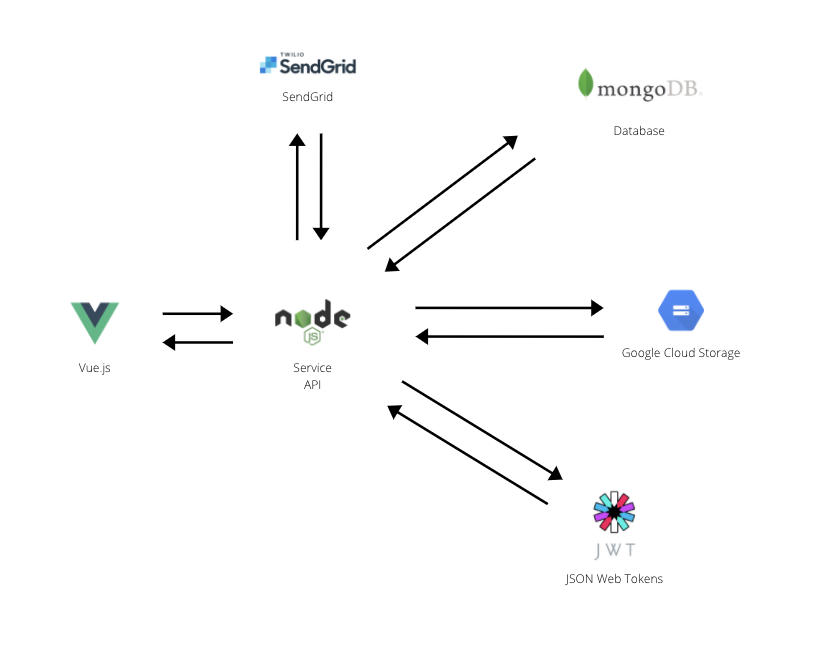
\includegraphics[width=0.9\columnwidth]{ExamaSystem.png}
  \caption{แสดงการทำงานขอเว็ปแอพพลิเคชั่นประเมินความสามารถเบื้องต้นของผู้สมัครงาน}
  \label{Fig:ExamaSystem}
\end{figure}

\newpage
\section{วิเคราะห์ความต้องการ}

\subsection{ความต้องการที่เป็นหน้าที่หลักของระบบ (Functional Requirement)}
\begin{enumerate}
  \item ผู้ใช้งานสามารถสามารถลงทะเบียนเป็นสมาชิกเพื่อใช้งานเว็บแอพพลิเคชั่นได้   
  \item ผู้ใช้ต้องยืนยันตัวตนผ่านอีเมลหลังจากทำการลงทะเบียน ถึงจะเข้าใช้งานระบบได้
  \item ผู้ใช้งานสามารถสร้าง, แก้ไข และลบคำถามในหมวดหมู่คำถามได้
  \item ระบบสามารถป้องกันการรีเฟรชเพจ หรือการเปลี่ยนหน้าได้ หากผู้ใช้กำลังสร้างหรือแก้ไขคำถามในหมวดหมู่คำถาม
  \item ผู้ใช้งานสามารถยกเลิกการสร้างหมวดหมู่คำถามได้
  \item ผู้ใช้งานไม่สามารถลบหมวดหมู่คำถามได้ หากหมวดหมู่นั้นถูกใช้งานอยู่ในข้อสอบ
  \item ผู้ใช้งานสามารถสร้างคำถามประเภท ปรนัย, อัตนัย และคำถามที่มีไฟล์แนบได้
  \item คำถามที่เป็นปรนัย สามารถเลือกให้มีข้อถูกมากกว่า 1 ข้อได้
  \item สามารถใส่รูปภาพเพิ่มในตัวเลือกคำตอบของคำถามประเภทปรนัยได้
  \item หากผู้ใช้งานส่งข้อสอบให้ผู้สมัครงานทำแล้ว ถ้าหมวดหมู่คำถามนั้นถูกใช้งานในข้อสอบ คำถามในหมวดหมู่นั้นจะสามารถแก้ไขได้เฉพาะเฉลยเท่านั้น ไม่สามารถแข้ไขคำถามได้ โดยหากต้องการแก้ไขให้ทำการคัดลอกหมวดหมู่คำถามของตนเองมาแก้ไขเป็นหมวดหมู่ใหม่
  \item ผู้ใช้งานสามารถคัดลอกหมวดหมู่คำถามของตนเองได้
  \item ผู้ใช้งานสามารถเปิดหมวดหมู่คำถามให้เป็นสาธารณะได้
  \item หมวดหมู่คำถามที่เป็นสาธารณะ ผู้ที่ไม่ใช้เจ้าของไม่สามารถแก้ไขได้ โดยผู้ใช้สามารถคัดลอกหมวดหมู่คำถามที่เป็นสาธารณะไปเป็นเป็นของตนเองได้ หากผู้ใช้ไม่ใช้เจ้าของแต่ต้องการแก้ไข
  \item ผู้ใช้งานสามารถค้นหาหมวดหมู่คำถามได้
  \item ผู้ใช้งานสามารถสร้างข้อสอบ ที่กำหนดหมวดหมู่คำถามที่ต้องการ,จำนวนข้อ และความยากได้ โดยข้อสอบจะทำการสุ่มเมื่อผู้ใช้ส่งให้ผู้ทำข้อสอบ
  \item ระบบสามารถป้องกันการรีเฟรชเพจ หรือการเปลี่ยนหน้าได้ หากผู้ใช้กำลังสร้างหรือแก้ไขข้อสอบ
  \item ผู้ใช้สามารถลบแก้ไขหมวดหมู่คำถามที่ใช้, จำนวนข้อ และระดับความยากของข้อสอบได้
  \item ผู้ใช้สามารถค้นหาข้อสอบได้
  \item ผู้ใช้สามารถเปิดข้อสอบให้เป็นสาธารณะได้
  \item ข้อสอบที่เป็นสาธารณะ ผู้ที่ไม่ใช้เจ้าของไม่สามารถแก้ไขได้ โดยผู้ใช้สามารถคัดลอกข้อสอบสาธารณะไปเป็นเป็นของตนเองได้ หากผู้ใช้ไม่ใช้เจ้าของแต่ต้องการแก้ไข
  \item หากผู้ใช้งานส่งข้อสอบให้ผู้สมัครงานทำแล้ว ข้อสอบที่ผู้ใช้งานสร้างขึ้นนั้นจะไม่สามารถแก้ไขได้ แต่สามารถส่งให้ผู้สมัครงานคนอื่นทำต่อไปได้ โดยระบบจะทำการสุ่มคำถามที่ผู้ออกข้อสอบกำหนด จำนวนข้อประเภทคำถาม และระดับความยาก
  \item ผู้ใช้งานสามารถดูประวัติที่ผู้ใช้ทำการส่งข้อสอบให้ผู้สมัครงานได้
  \item ผู้ใช้สามารถกำหนดระยะเวลาการทำข้อสอบได้
  \item ผู้ใช้สามารถกำหนดวันหมดอายุของข้อสอบได้
  \item ผู้ใช้สามารถส่งข้อสอบให้ผู้สมัครงานผ่านอีเมลได้
  \item ผู้ทำข้อสอบสามารถเข้ามาทำข้อสอบในเว็บแอพพลิเคชั่นได้ตลอด หากเวลาในการทำข้อสอบยังไม่หมด
  \item เมื่อผู้ทำข้อสอบทำการส่งข้อสอบแล้ว ระบบสามารถตรวจข้อสอบที่เป็นปรนัยได้
  \item มีการแสดงสถานะบอกว่าผู้ใช้งาน ตรวจข้อสอบนั้นหรือยัง
  \item มีการสรุปคะแนนรวมข้อผู้ทำข้อสอบ
\end{enumerate}

\newcolumntype{L}[1]{>{\raggedright\let\newline\\\arraybackslash}p{#1}}

\section{การวิเคราะห์และออกแบบระบบ}

\subsection{แผนภาพยูสเคส (Use Case Diagram)}

\begin{figure}[H]
  \centering
  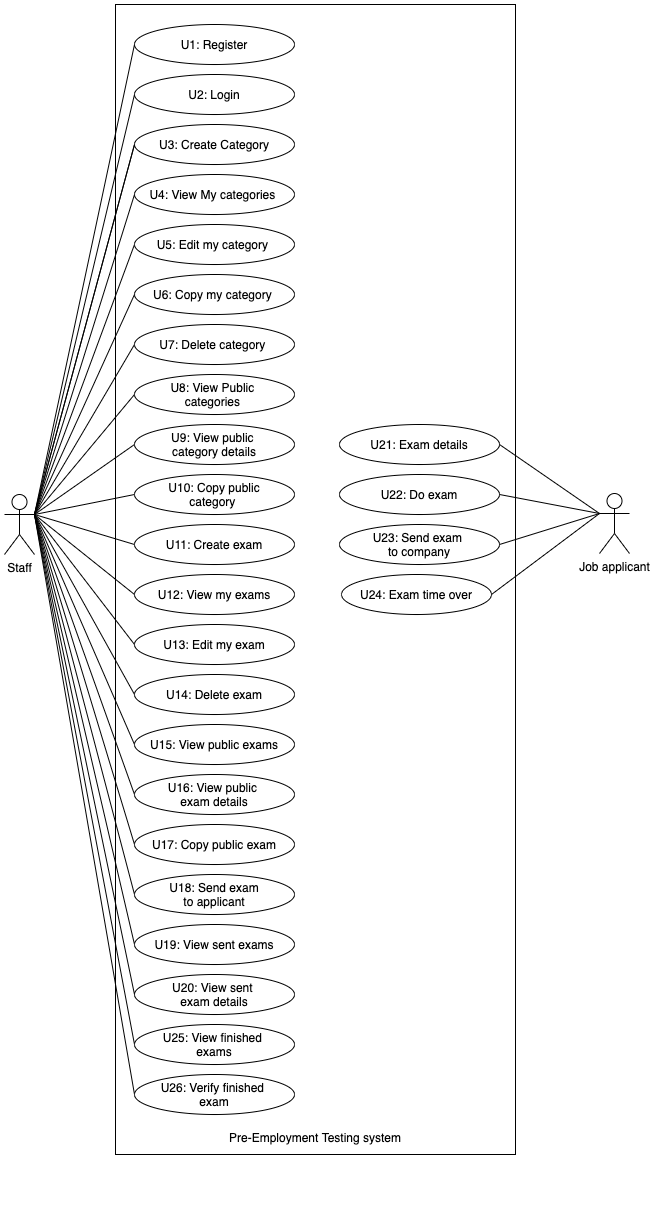
\includegraphics[width=0.78\columnwidth]{examaUseCaseDiagram .png}
  \caption{แผนภาพยูสเคสของระบบ}
  \label{Fig:examaUseCaseDiagram}
\end{figure}

\subsection{รายละเอียดการทำงานในแต่ละยูสเคศ (Use Case Description)}

\subsubsection{รายละเอียดยูสเคส ลงทะเบียน}

\begin{table}[H]
  \begin{tabular}{|l|l|l|} 
  \hline
  Use Case No:                                      & \multicolumn{2}{l|}{1}\\ 
  \hline
  Use Case Name:                                    & \multicolumn{2}{l|}{ลงทะเบียน}\\
  \hline
  Use Case~Scenario:                                & \multicolumn{2}{l|}{ผู้ใช้ลงทะเบียนกับระบบ}\\ 
  \hline
  \vcell{Triggering Event:}                         & \multicolumn{2}{l|}{\vcell{\begin{tabular}[b]{@{}l@{}}เมื่อผู้ใช้เข้าใช้งานเป็นครั้งแรก\end{tabular}}}\\[-\rowheight]
  \printcelltop                                     & \multicolumn{2}{l|}{\printcellmiddle}\\
  \hline
  Brief Description:                                & \multicolumn{2}{l|}{สำหรับให้ผู้ใช้ลงทะเบียนเข้าสู้ระบบ}\\ 
  \hline
  Actors:                                           & \multicolumn{2}{l|}{พนักงาน}\\ 
  \hline
  Related Use Cases:                                & \multicolumn{2}{l|}{-}\\ 
  \hline
  Stakeholders:                                     & \multicolumn{2}{l|}{-}\\ 
  \hline
  Pre - Conditions:                                 & \multicolumn{2}{l|}{-}\\ 
  \hline
  Post - Conditions:                                & \multicolumn{2}{l|}{ผู้ใช้สามารถเข้าใช้งานระบบได้}\\ 
  \hline
  Flow of Events:                                   & \multicolumn{1}{c|}{ผู้ใช้} & \multicolumn{1}{c|}{ระบบ}\\  
  \cline{2-3}
                                                    & \vcell{\begin{tabular}[b]{m{0.28\linewidth}}
                                                      1.ผู้ใช้เลือกลงทะเบียน\\\\\\
                                                      3.ผู้ใช้ทำการกรอกชื่อ-\\นามสกุล,อีเมล,รหัสผ่าน \\และยืนยันรหัสผ่าน แล้ว\\ทำการคลิกลงทะเบียน\\\\\\
                                                      5.ผู้ใช้งานได้รับอีเมล แล้ว\\ทำการคลิกลิงค์เว็บไซต์\\\\\\\\
                                                      \end{tabular}}
                                                    & \vcell{\begin{tabular}[b]{m{0.28\linewidth}}
                                                      \\
                                                      2.ระบบแสดงแบบฟอร์มให้กรอกข้อมูล\\\\\\\\\\
                                                      4.ระบบทำการส่งอีเมลให้ผู้\\ใช้เพื่อทำการยืนยันอีเมล\\\\\\
                                                      6.ระบบทำการยืนยันอีเมล\\ แล้วแสดงหน้าจอหลักของผู้ใช้งาน
                                                      \end{tabular}}\\[-\rowheight]
                                                    & \printcelltop & \printcelltop\\ 
  \hline
  \vcell{Exception Conditions:}                     & \multicolumn{2}{l|}{\vcell{\begin{tabular}[b]{@{}l@{}}- ผู้ใช้กรอกรายละเอียดไม่ครบถ้วน หรือไม่ตรงเงื่อนไข\\- ผู้ใช้ไม่ได้ทำการยืนยันอีเมล\\- ผู้ใช้กรอกอีเมลที่ไม่มีอยู่จริง\\- ผู้ใช้กรอกออีเมลที่ผู้ใช้งานไม่สามารถเข้าใช้อีเมลนั้นได้\end{tabular}}}\\[-\rowheight]
  \printcelltop                                     & \multicolumn{2}{l|}{\printcellmiddle}\\
  \hline
  \end{tabular}
  \caption{รายละเอียดยูสเคส ลงทะเบียน}
  \label{Table:register}
\end{table}

\subsubsection{รายละเอียดยูสเคส เข้าสู่ระบบ}

\begin{table}[H]
  \begin{tabular}{|l|l|l|} 
  \hline
  Use Case No:                                      & \multicolumn{2}{l|}{2}\\ 
  \hline
  Use Case Name:                                    & \multicolumn{2}{l|}{เข้าสู่ระบบ}\\
  \hline
  Use Case~Scenario:                                & \multicolumn{2}{l|}{ผู้ใช้ต้องการเข้าสู่ระบบ}\\ 
  \hline
  \vcell{Triggering Event:}                         & \multicolumn{2}{l|}{\vcell{\begin{tabular}[b]{@{}l@{}}- เมื่อผู้ใช้ต้องการเข้าใช้งานระบบ\\- ผู้ใช้เข้าเว็ปแอพพลิเคชั่นโดยที่ยังไม่เข้าใช้งานระบบ\end{tabular}}}\\[-\rowheight]
  \printcelltop                                     & \multicolumn{2}{l|}{\printcellmiddle}\\
  \hline
  Brief Description:                                & \multicolumn{2}{l|}{สำหรับให้ผู้ใช้เข้าสู่ระบบเพื่อเข้าใช้งานเว็ปแอปพลิเคชั่น}\\ 
  \hline
  Actors:                                           & \multicolumn{2}{l|}{พนักงาน}\\ 
  \hline
  Related Use Cases:                                & \multicolumn{2}{l|}{ลงทะเบียน}\\ 
  \hline
  Stakeholders:                                     & \multicolumn{2}{l|}{-}\\ 
  \hline
  Pre - Conditions:                                 & \multicolumn{2}{l|}{ผู้ใช้ต้องทำการลงทะเบียนและยืนยันตัวตนผ่านอีเมลเรียบร้อยแล้ว}\\ 
  \hline
  Post - Conditions:                                & \multicolumn{2}{l|}{ระบบแสดงหน้าจอสำหรับผู้ใช้งาน}\\ 
  \hline
  Flow of Events:                                   & \multicolumn{1}{c|}{ผู้ใช้} & \multicolumn{1}{c|}{ระบบ}\\  
  \cline{2-3}
                                                    & \vcell{\begin{tabular}[b]{m{0.28\linewidth}}
                                                      1.ผู้ใช้เข้าหน้าเว็ปโดยที่ยังไม่ได้ทำการเข้าสู้ระบบ\\\\\\
                                                      3.ผู้ใช้ทำการกรอกอีเมล และรหัสผ่านแล้วทำการคลิกเข้าสู่ระบบ หรือกด Enter บนแป้นพิมพ์\\\\\\
                                                      \end{tabular}}
                                                    & \vcell{\begin{tabular}[b]{m{0.28\linewidth}}
                                                      \\\\
                                                      2.ระบบแสดงแบบฟอร์มให้กรอกข้อมูล\\\\\\\\\\
                                                      4.ระบบแสดงหน้าจอหลักของผู้ใช้งาน
                                                      \end{tabular}}\\[-\rowheight]
                                                    & \printcelltop & \printcelltop\\ 
  \hline
  \vcell{Exception Conditions:}                     & \multicolumn{2}{l|}{\vcell{\begin{tabular}[b]{@{}l@{}}ผู้ใช้กรอกอีเมล หรือรหัสผ่านผิด\end{tabular}}}\\[-\rowheight]
  \printcelltop                                     & \multicolumn{2}{l|}{\printcellmiddle}\\
  \hline
  \end{tabular}
  \caption{รายละเอียดยูสเคส เข้าสู่ระบบ}
  \label{Table:login}
\end{table}

\subsubsection{รายละเอียดยูสเคส สร้างหมวดหมู่คำถาม}

\begin{table}[H]
  \begin{tabular}{|l|l|l|} 
  \hline
  Use Case No:                                      & \multicolumn{2}{l|}{3}\\ 
  \hline
  Use Case Name:                                    & \multicolumn{2}{l|}{สร้างหมวดหมู่คำถาม}\\
  \hline
  Use Case~Scenario:                                & \multicolumn{2}{l|}{ผู้ใช้ต้องการงหมวดหมู่คำถาม}\\
  \hline
  \vcell{Triggering Event:}                         & \multicolumn{2}{l|}{\vcell{\begin{tabular}[b]{@{}l@{}}เมื่อผู้ใช้ต้องการสร้างหมวดหมู่คำถาม ไว้ใช้ในข้อสอบของ\\ตนเอง หรือให้พนักงานคนอื่นใช้\end{tabular}}}\\[-\rowheight]
  \printcelltop                                     & \multicolumn{2}{l|}{\printcellmiddle}\\
  \hline
  \vcell{Brief Description:}                        & \multicolumn{2}{l|}{\vcell{\begin{tabular}[b]{@{}l@{}}สำหรับให้ผู้ใช้ ออกข้อสอบโดยแบ่งแยกตามแต่ละหมวดหมู่ เช่น\\คณิตศาสตร์, โปรแกรมมิ่ง หรือ แบบทดสอบสติปัญญา โดยมีชนิด\\คำถามแบ่งออกเป็น อัตนัย, ปรนัย และคำถามที่มีไฟล์แนบ\end{tabular}}}\\[-\rowheight]
  \printcelltop                                     & \multicolumn{2}{l|}{\printcellmiddle}\\
  \hline
  Actors:                                           & \multicolumn{2}{l|}{พนักงาน}\\ 
  \hline
  Related Use Cases:                                & \multicolumn{2}{l|}{เข้าสู่ระบบ}\\ 
  \hline
  Stakeholders:                                     & \multicolumn{2}{l|}{-}\\ 
  \hline
  Pre - Conditions:                                 & \multicolumn{2}{l|}{ผู้ใช้ต้องทำการเข้าสู่ระบบ}\\ 
  \hline
  \vcell{Post - Conditions:}                        & \multicolumn{2}{l|}{\vcell{\begin{tabular}[b]{@{}l@{}}ผู้ใช้มีหมวดหมู่คำถามที่ตนเองสร้างขึ้น และแสดงหน้าหมวด\\หมู่ทั้งหมดของผู้ใช้\end{tabular}}}\\[-\rowheight]
  \printcelltop                                     & \multicolumn{2}{l|}{\printcellmiddle}\\
  \hline
  Flow of Events:                                   & \multicolumn{1}{c|}{ผู้ใช้} & \multicolumn{1}{c|}{ระบบ}\\  
  \cline{2-3}
                                                    & \vcell{\begin{tabular}[b]{m{0.28\linewidth}}
                                                      1.ไปที่หน้าสร้างหมวดหมู่\\\\\\
                                                      3.ผู้ใช้กรอกชื่อหมวดหมู่\\และกรอกหัวเรื่อง\\
                                                      4.สร้างคำถามภายใต้ หมวดหมู่นั้นโดยสามารถเลือก\\ระดับความยาก และประเภทของคำถาม แล้วทำการคลิกสร้างหมวดหมู่\\\\\\\\                                                
                                                      \end{tabular}}
                                                    & \vcell{\begin{tabular}[b]{m{0.28\linewidth}}
                                                      \\
                                                      2.ระบบแสดงหน้าสร้าง\\หมวดหมู่คำถาม\\\\\\\\\\\\\\\\
                                                      5.ระบบทำการสร้างหมดหมู่คำถาม แล้วแสดงหน้าหมวด\\หมู่คำถามทั้งหมดของผู้ใช้
                                                      \end{tabular}}\\[-\rowheight]
                                                    & \printcelltop & \printcelltop\\ 
  \hline
  \vcell{Exception Conditions:}                     & \multicolumn{2}{l|}{\vcell{\begin{tabular}[b]{@{}l@{}}- ผู้ใช้กรอกขื่อหมวดหมู่ซ้ำกับ หมวดหมู่ที่ตนเองมีอยู่แล้ว\\- ผู้ใช้กรอกข้อมูลไม่ครบ ตามฟอร์มที่ให้กรอก\\- ไฟล์ที่แนบมามีขนาดใหญ่เกินที่กำหนด หรือประเภทของไฟล์ไม่\\\hspace{0.22cm}ถูกต้อง\end{tabular}}}\\[-\rowheight]
  \printcelltop                                     & \multicolumn{2}{l|}{\printcellmiddle}\\
  \hline
  \end{tabular}
  \caption{รายละเอียดยูสเคส สร้างหมวดหมู่คำถาม}
  \label{Table:createCategory}
\end{table}

\subsubsection{รายละเอียดยูสเคส ดูหมวดหมู่คำถามของผู้ใช้}

\begin{table}[H]
  \begin{tabular}{|l|l|l|} 
  \hline
  Use Case No:                                      & \multicolumn{2}{l|}{4}\\ 
  \hline
  Use Case Name:                                    & \multicolumn{2}{l|}{ดูหมวดหมู่คำถามของผู้ใช้}\\
  \hline
  Use Case~Scenario:                                & \multicolumn{2}{l|}{ผู้ใช้ต้องการดูหมวดหมู่คำถามของตนเอง}\\ 
  \hline
  \vcell{Triggering Event:}                         & \multicolumn{2}{l|}{\vcell{\begin{tabular}[b]{@{}l@{}}- เมื่อผู้ใช้ต้องการดูหมวดหมู่คำถามของตนเอง\\- เมื่อผู้ใช้สร้างประเภทของข้อสอบสำเร็จ หน้าเว็ปจะทำการไป\\\hspace{0.22cm}แสดงผลที่หน้าหมวดหมู่คำถามทั้งหมเของผู้ใช้\end{tabular}}}\\[-\rowheight]
  \printcelltop                                     & \multicolumn{2}{l|}{\printcellmiddle}\\
  \hline
  \vcell{Brief Description:}                        & \multicolumn{2}{l|}{\vcell{\begin{tabular}[b]{@{}l@{}}สำหรับให้ผู้ใช้งานดูหมวดหมู่คำถามที่ตนเองสร้างขึ้น หรือ\\หมวดหมู่คำถามที่คัดลอกมาจากหมวดหมู่สาธารณะ\end{tabular}}}\\[-\rowheight]
  \printcelltop                                     & \multicolumn{2}{l|}{\printcellmiddle}\\
  \hline
  Actors:                                           & \multicolumn{2}{l|}{พนักงาน}\\ 
  \hline
  \vcell{Related Use Cases:}                        & \multicolumn{2}{l|}{\vcell{\begin{tabular}[b]{@{}l@{}}เข้าสู่ระบบ, สร้างหมวดหมู่คำถาม, คัดลอกหมวดหมู่คำถาม\\จากหมวดหมู่คำถามสาธารณะ\end{tabular}}}\\[-\rowheight]
  \printcelltop                                     & \multicolumn{2}{l|}{\printcellmiddle}\\
  \hline
  Stakeholders:                                     & \multicolumn{2}{l|}{-}\\ 
  \hline
  \vcell{Pre - Conditions:}                         & \multicolumn{2}{l|}{\vcell{\begin{tabular}[b]{@{}l@{}}- ผู้ใช้ต้องทำการเข้าสู่ระบบ\\- สร้างหมวดหมู่คำถาม หรือคัดลอกหมวดหมู่คำถามจาก\\\hspace{0.22cm}หมวดหมู่คำถามสาธารณะ\end{tabular}}}\\[-\rowheight]
  \printcelltop                                     & \multicolumn{2}{l|}{\printcellmiddle}\\
  \hline
  \vcell{Post - Conditions:}                        & \multicolumn{2}{l|}{\vcell{\begin{tabular}[b]{@{}l@{}}แสดงหน้าหมวดหมู่ทั้งหมดของผู้ใช้\end{tabular}}}\\[-\rowheight]
  \printcelltop                                     & \multicolumn{2}{l|}{\printcellmiddle}\\
  \hline
  Flow of Events:                                   & \multicolumn{1}{c|}{ผู้ใช้} & \multicolumn{1}{c|}{ระบบ}\\  
  \cline{2-3}
                                                    & \vcell{\begin{tabular}[b]{m{0.28\linewidth}}
                                                      1.ไปที่หน้าดูหมวดหมู่คำ\\ถามของผู้ใช้                                            
                                                      \end{tabular}}
                                                    & \vcell{\begin{tabular}[b]{m{0.28\linewidth}}
                                                      \\\\
                                                      2.ระบบแสดงหมวดหมู่\\ทั้งหมดของผู้ใช้
                                                      \end{tabular}}\\[-\rowheight]
                                                    & \printcelltop & \printcelltop\\ 
  \hline
  \vcell{Exception Conditions:}                     & \multicolumn{2}{l|}{\vcell{\begin{tabular}[b]{@{}l@{}}ผู้ใช้ไม่มีหมวดหมู่คำถาม\end{tabular}}}\\[-\rowheight]
  \printcelltop                                     & \multicolumn{2}{l|}{\printcellmiddle}\\
  \hline
  \end{tabular}
  \caption{รายละเอียดยูสเคส ดูหมวดหมู่คำถามของผู้ใช้}
  \label{Table:viewMyCategory}
\end{table}

\subsubsection{รายละเอียดยูสเคส แก้ไขหมวดหมู่คำถามของผู้ใช้}

\begin{table}[H]
  \begin{tabular}{|l|l|l|} 
  \hline
  Use Case No:                                      & \multicolumn{2}{l|}{5}\\ 
  \hline
  Use Case Name:                                    & \multicolumn{2}{l|}{แก้ไขหมวดหมู่คำถามของผู้ใช้}\\
  \hline
  Use Case~Scenario:                                & \multicolumn{2}{l|}{ผู้ใช้ต้องการแก้ไขหมวดหมู่คำถามของตนเอง}\\ 
  \hline
  \vcell{Triggering Event:}                         & \multicolumn{2}{l|}{\vcell{\begin{tabular}[b]{@{}l@{}}เมื่อผู้ใช้ต้องการแก้ไขรายละเอียดในหมวดหมู่คำถาม เช่นเพิ่มคำ\\ถาม, แก้ไขคำถาม หรือแก้ไขชื่อหมวดหมู่\end{tabular}}}\\[-\rowheight]
  \printcelltop                                     & \multicolumn{2}{l|}{\printcellmiddle}\\
  \hline
  \vcell{Brief Description:}                        & \multicolumn{2}{l|}{\vcell{\begin{tabular}[b]{@{}l@{}}สำหรับให้ผู้ใช้งานแก้ไขรายละเอียดต่างๆในหมวดหมู่คำถาม\end{tabular}}}\\[-\rowheight]
  \printcelltop                                     & \multicolumn{2}{l|}{\printcellmiddle}\\
  \hline
  Actors:                                           & \multicolumn{2}{l|}{พนักงาน}\\ 
  \hline
  \vcell{Related Use Cases:}                        & \multicolumn{2}{l|}{\vcell{\begin{tabular}[b]{@{}l@{}}เข้าสู่ระบบ, สร้างหมวดหมู่คำถาม, คัดลอกหมวดหมู่คำถาม\\จากหมวดหมู่คำถามสาธารณะ\end{tabular}}}\\[-\rowheight]
  \printcelltop                                     & \multicolumn{2}{l|}{\printcellmiddle}\\
  \hline
  Stakeholders:                                     & \multicolumn{2}{l|}{-}\\ 
  \hline
  \vcell{Pre - Conditions:}                         & \multicolumn{2}{l|}{\vcell{\begin{tabular}[b]{@{}l@{}}- ผู้ใช้ต้องทำการเข้าสู่ระบบ\\- สร้างหมวดหมู่คำถาม หรือคัดลอกหมวดหมู่คำถามจาก\\\hspace{0.22cm}หมวดหมู่คำถามสาธารณะ\end{tabular}}}\\[-\rowheight]
  \printcelltop                                     & \multicolumn{2}{l|}{\printcellmiddle}\\
  \hline
  \vcell{Post - Conditions:}                        & \multicolumn{2}{l|}{\vcell{\begin{tabular}[b]{@{}l@{}}แสดงหน้าหมวดหมู่ทั้งหมดของผู้ใช้\end{tabular}}}\\[-\rowheight]
  \printcelltop                                     & \multicolumn{2}{l|}{\printcellmiddle}\\
  \hline
  Flow of Events:                                   & \multicolumn{1}{c|}{ผู้ใช้} & \multicolumn{1}{c|}{ระบบ}\\  
  \cline{2-3}
                                                    & \vcell{\begin{tabular}[b]{m{0.28\linewidth}}
                                                      1.ไปที่หน้าดูหมวดหมู่คำ\\ถามของผู้ใช้\\\\\\
                                                      3.คลิกที่หมวดหมู่คำถาม\\ที่ต้องการแก้ไข\\\\\\
                                                      5.ผู้ใช้ทำการแก้ไขข้อมูล\\ต่างๆในประเภทที่ต้องการ\\ แล้วทำการคลิกยืนยันการ\\แก้ไข\\\\\\\\
                                                      \end{tabular}}
                                                    & \vcell{\begin{tabular}[b]{m{0.28\linewidth}}
                                                      \\\\
                                                      2.ระบบแสดงหมวดหมู่\\ทั้งหมดของผู้ใช้\\\\\\
                                                      4.ระบบแสดงหน้าแก้ไข\\หมวดหมู่นั้นๆ\\\\\\\\\\
                                                      6.ระบบทำการแก้ไขข้อมูล\\
                                                      7.ระบบแสดงหน้าหมวดหมู่ทั้งหมดของผู้ใช้\\
                                                      \end{tabular}}\\[-\rowheight]
                                                    & \printcelltop & \printcelltop\\ 
  \hline
  \vcell{Exception Conditions:}                     & \multicolumn{2}{l|}{\vcell{
                                                        \begin{tabular}[b]{@{}l@{}}
                                                          - ผู้ใช้กรอกชื่อหมวดหมู่ซ้ำกับ หมวดหมู่ที่ตนเองมีอยู่แล้ว\\
                                                          - ผู้ใช้กรอกรายละเอียดไม่ครบถ้วน หรือไม่ตรงเงื่อนไข\\
                                                          - ไฟล์ที่แนบมามีขนาดใหญ่เกินที่กำหนด หรือประเภทของไฟล์\\\hspace{0.22cm}ไม่ถูกต้อง\\
                                                          - สามารถแก้ไขได้เฉพาะคำตอบ หากข้อสอบเคยถูกใช้ไปแล้ว
                                                        \end{tabular}}}\\[-\rowheight]
  \printcelltop                                     & \multicolumn{2}{l|}{\printcellmiddle}\\
  \hline
  \end{tabular}
  \caption{รายละเอียดยูสเคส แก้ไขหมวดหมู่คำถามของผู้ใช้}
  \label{Table:editMyCategory}
\end{table}

\subsubsection{รายละเอียดยูสเคส คัดลอกหมวดหมู่คำถามของผู้ใช้}

\begin{table}[H]
  \begin{tabular}{|l|l|l|} 
  \hline
  Use Case No:                                      & \multicolumn{2}{l|}{6}\\ 
  \hline
  Use Case Name:                                    & \multicolumn{2}{l|}{คัดลอกหมวดหมู่คำถามของผู้ใช้}\\
  \hline
  Use Case~Scenario:                                & \multicolumn{2}{l|}{ผู้ใช้ต้องการคัดลอกหมวดหมู่คำถามของตนเอง}\\ 
  \hline
  \vcell{Triggering Event:}                         & \multicolumn{2}{l|}{\vcell{\begin{tabular}[b]{@{}l@{}}เมื่อผู้ใช้ต้องการแก้ไขหมวดหมู่คำถามที่ถูกส่งให้ผู้สมัครงาน\\แล้ว ทำให้ไม่สามารถแก้ไขหมวดหมู่เดิมได้ หรือต้องการคัดลอก\\หมวดหมู่มาแก้ไข โดยที่ไม่ต้องการให้กระทบหมวดหมู่เดิม\end{tabular}}}\\[-\rowheight]
  \printcelltop                                     & \multicolumn{2}{l|}{\printcellmiddle}\\
  \hline
  \vcell{Brief Description:}                        & \multicolumn{2}{l|}{\vcell{\begin{tabular}[b]{@{}l@{}}สำหรับให้ผู้ใช้งานคัดลอกหมวดหมู่คำถามของตนเอง\end{tabular}}}\\[-\rowheight]
  \printcelltop                                     & \multicolumn{2}{l|}{\printcellmiddle}\\
  \hline
  Actors:                                           & \multicolumn{2}{l|}{พนักงาน}\\ 
  \hline
  \vcell{Related Use Cases:}                        & \multicolumn{2}{l|}{\vcell{\begin{tabular}[b]{@{}l@{}}เข้าสู่ระบบ, สร้างหมวดหมู่คำถาม, ส่งข้อสอบให้ผู้สมัคร\end{tabular}}}\\[-\rowheight]
  \printcelltop                                     & \multicolumn{2}{l|}{\printcellmiddle}\\
  \hline
  Stakeholders:                                     & \multicolumn{2}{l|}{-}\\ 
  \hline
  \vcell{Pre - Conditions:}                         & \multicolumn{2}{l|}{\vcell{\begin{tabular}[b]{@{}l@{}}- ผู้ใช้ต้องทำการเข้าสู่ระบบ\\- สร้างหมวดหมู่คำถาม หรือคัดลอกหมวดหมู่คำถามจาก\\\hspace{0.22cm}หมวดหมู่คำถามสาธารณะ\end{tabular}}}\\[-\rowheight]
  \printcelltop                                     & \multicolumn{2}{l|}{\printcellmiddle}\\
  \hline
  \vcell{Post - Conditions:}                        & \multicolumn{2}{l|}{\vcell{\begin{tabular}[b]{@{}l@{}}ระบบทำการคัดลอกหหมวดหมู่คำถามที่ผู้ใช้ต้องการ\end{tabular}}}\\[-\rowheight]
  \printcelltop                                     & \multicolumn{2}{l|}{\printcellmiddle}\\
  \hline
  Flow of Events:                                   & \multicolumn{1}{c|}{ผู้ใช้} & \multicolumn{1}{c|}{ระบบ}\\  
  \cline{2-3}
                                                    & \vcell{\begin{tabular}[b]{m{0.28\linewidth}}
                                                      1.ไปที่หน้าดูหมวดหมู่\\คำถามของผู้ใช้\\\\\\
                                                      3.คลิกปุ่มคักลอกที่หมวด\\หมู่ที่ต้องการคัดลอก\\\\\\
                                                      5.ผู้ใช้งานกดยืนยันการคัด\\ลอก\\\\\\
                                                      \end{tabular}}
                                                    & \vcell{\begin{tabular}[b]{m{0.28\linewidth}}
                                                      \\\\
                                                      2.ระบบแสดงหมวดหมู่\\ทั้งหมดของผู้ใช้\\\\\\
                                                      4.ระบบแสดงหน้ายืนยันการคัดลอก\\\\\\
                                                      6.ระบบทำการคัดลอกหมวดหมู่คำถามนั้น\\
                                                      \end{tabular}}\\[-\rowheight]
                                                    & \printcelltop & \printcelltop\\ 
  \hline
  \vcell{Exception Conditions:}                     & \multicolumn{2}{l|}{\vcell{
                                                        \begin{tabular}[b]{@{}l@{}}
                                                          ผู้ใช้ไม่มีหมวดหมู่คำถาม
                                                        \end{tabular}}}\\[-\rowheight]
  \printcelltop                                     & \multicolumn{2}{l|}{\printcellmiddle}\\
  \hline
  \end{tabular}
  \caption{รายละเอียดยูสเคส คัดลอกหมวดหมู่คำถามของผู้ใช้}
  \label{Table:copyMyCategory}
\end{table}

\subsubsection{รายละเอียดยูสเคส ลบหมวดหมู่คำถามของผู้ใช้}

\begin{table}[H]
  \begin{tabular}{|l|l|l|} 
  \hline
  Use Case No:                                      & \multicolumn{2}{l|}{7}\\ 
  \hline
  Use Case Name:                                    & \multicolumn{2}{l|}{ลบหมวดหมู่คำถามของผู้ใช้}\\
  \hline
  Use Case~Scenario:                                & \multicolumn{2}{l|}{ผู้ใช้ต้องการลบหมวดหมู่คำถามของตนเอง}\\ 
  \hline
  \vcell{Triggering Event:}                         & \multicolumn{2}{l|}{\vcell{\begin{tabular}[b]{@{}l@{}}เมื่อผู้ใช้ไม่ต้องการหมวดหมู่คำถามนั้นๆแล้ว\end{tabular}}}\\[-\rowheight]
  \printcelltop                                     & \multicolumn{2}{l|}{\printcellmiddle}\\
  \hline
  \vcell{Brief Description:}                        & \multicolumn{2}{l|}{\vcell{\begin{tabular}[b]{@{}l@{}}สำหรับให้ผู้ใช้งานลบหมวดหมู่คำถามออกจากหมวดหมู่คำถาม\\ของตนเอง\end{tabular}}}\\[-\rowheight]
  \printcelltop                                     & \multicolumn{2}{l|}{\printcellmiddle}\\
  \hline
  Actors:                                           & \multicolumn{2}{l|}{พนักงาน}\\ 
  \hline
  \vcell{Related Use Cases:}                        & \multicolumn{2}{l|}{\vcell{\begin{tabular}[b]{@{}l@{}}เข้าสู่ระบบ, สร้างหมวดหมู่คำถาม, คัดลอกหมวดหมู่คำถาม\\จากหมวดหมู่คำถามสาธารณะ, ข้อสอบของผู้ใช้\end{tabular}}}\\[-\rowheight]
  \printcelltop                                     & \multicolumn{2}{l|}{\printcellmiddle}\\
  \hline
  Stakeholders:                                     & \multicolumn{2}{l|}{-}\\ 
  \hline
  \vcell{Pre - Conditions:}                         & \multicolumn{2}{l|}{\vcell{\begin{tabular}[b]{@{}l@{}}- ผู้ใช้ต้องทำการเข้าสู่ระบบ\\- สร้างหมวดหมู่คำถาม หรือคัดลอกหมวดหมู่คำถามจาก\\\hspace{0.22cm}หมวดหมู่สาธารณะ\end{tabular}}}\\[-\rowheight]
  \printcelltop                                     & \multicolumn{2}{l|}{\printcellmiddle}\\
  \hline
  \vcell{Post - Conditions:}                        & \multicolumn{2}{l|}{\vcell{\begin{tabular}[b]{@{}l@{}}ระบบลบหมวดหมู่คำถามของผู้ใช้\end{tabular}}}\\[-\rowheight]
  \printcelltop                                     & \multicolumn{2}{l|}{\printcellmiddle}\\
  \hline
  Flow of Events:                                   & \multicolumn{1}{c|}{ผู้ใช้} & \multicolumn{1}{c|}{ระบบ}\\  
  \cline{2-3}
                                                    & \vcell{\begin{tabular}[b]{m{0.28\linewidth}}
                                                      1.ไปที่หน้าดูหมวดหมู่คำ\\ถามของผู้ใช้\\\\\\
                                                      3.คลิกที่รูปถึงขยะของ\\หมวดหมู่คำถามที่ต้องการลบ\\\\\\\\
                                                      5.ผู้ใช้ทำการยืนยันการลบ\\\\\\
                                                      \end{tabular}}
                                                    & \vcell{\begin{tabular}[b]{m{0.28\linewidth}}
                                                      \\\\
                                                      2.ระบบแสดงหมวดหมู่\\ทั้งหมดของผู้ใช้\\\\\\\\
                                                      4.ระบบทำการแสดง\\หน้าต่างข้อความยืนยัน\\การลบ\\\\
                                                      6.ระบบทำการลบหมวดหมู่คำถามที่ผู้ใช้ต้องการลบ\\
                                                      \end{tabular}}\\[-\rowheight]
                                                    & \printcelltop & \printcelltop\\ 
  \hline
  \vcell{Exception Conditions:}                     & \multicolumn{2}{l|}{\vcell{
                                                        \begin{tabular}[b]{@{}l@{}}
                                                          - ผู้ใช้ไม่ทำการยืนยันการลบ\\
                                                          - หมวดหมู่คำถามที่ต้องการลบ ถูกใช้งานอยู่ในข้อสอบ ทำให้ไม่\\
                                                          \hspace{0.22cm}สามารถลบได้
                                                        \end{tabular}}}\\[-\rowheight]
  \printcelltop                                     & \multicolumn{2}{l|}{\printcellmiddle}\\
  \hline
  \end{tabular}
  \caption{รายละเอียดยูสเคส ลบหมวดหมู่คำถามของผู้ใช้}
  \label{Table:deleteCategory}
\end{table}

\subsubsection{รายละเอียดยูสเคส ดูหมวดหมู่คำถามสาธารณะ}

\begin{table}[H]
  \begin{tabular}{|l|l|l|} 
  \hline
  Use Case No:                                      & \multicolumn{2}{l|}{8}\\ 
  \hline
  Use Case Name:                                    & \multicolumn{2}{l|}{ดูหมวดหมู่คำถามสาธารณะ}\\
  \hline
  Use Case~Scenario:                                & \multicolumn{2}{l|}{ผู้ใช้ต้องการดูหมวดหมู่คำถามสาธารณะ}\\ 
  \hline
  \vcell{Triggering Event:}                         & \multicolumn{2}{l|}{\vcell{
                                                        \begin{tabular}[b]{@{}l@{}}
                                                          - เมื่อผู้ใช้ต้องการดูหมวดหมู่คำถามสาธารณะ\\
                                                          - เมื่อผู้ใช้ต้องการนำหมวดหมู่คำถามสาธารณะไปใช้ในข้อสอบ\\
                                                          \hspace{0.22cm}ของตนเอง
                                                        \end{tabular}}}\\[-\rowheight]
  \printcelltop                                     & \multicolumn{2}{l|}{\printcellmiddle}\\
  \hline
  \vcell{Brief Description:}                        & \multicolumn{2}{l|}{\vcell{\begin{tabular}[b]{@{}l@{}}สำหรับให้ผู้ใช้ดูว่ามีหมวดหมู่คำถามสาธารณะใดบ้างที่อยู่ใน\\ระบบและสามารถคัดลอกไปใช้ได้\end{tabular}}}\\[-\rowheight]
  \printcelltop                                     & \multicolumn{2}{l|}{\printcellmiddle}\\
  \hline
  Actors:                                           & \multicolumn{2}{l|}{พนักงาน}\\ 
  \hline
  \vcell{Related Use Cases:}                        & \multicolumn{2}{l|}{\vcell{\begin{tabular}[b]{@{}l@{}}เข้าสู่ระบบ\end{tabular}}}\\[-\rowheight]
  \printcelltop                                     & \multicolumn{2}{l|}{\printcellmiddle}\\
  \hline
  Stakeholders:                                     & \multicolumn{2}{l|}{-}\\ 
  \hline
  \vcell{Pre - Conditions:}                         & \multicolumn{2}{l|}{\vcell{\begin{tabular}[b]{@{}l@{}}ผู้ใช้ต้องทำการเข้าสู่ระบบ\end{tabular}}}\\[-\rowheight]
  \printcelltop                                     & \multicolumn{2}{l|}{\printcellmiddle}\\
  \hline
  \vcell{Post - Conditions:}                        & \multicolumn{2}{l|}{\vcell{\begin{tabular}[b]{@{}l@{}}ระบบแสดงหมวดหมูข้อสอบทั้งหมด ที่เป็นสาธารณะ\end{tabular}}}\\[-\rowheight]
  \printcelltop                                     & \multicolumn{2}{l|}{\printcellmiddle}\\
  \hline
  Flow of Events:                                   & \multicolumn{1}{c|}{ผู้ใช้} & \multicolumn{1}{c|}{ระบบ}\\  
  \cline{2-3}
                                                    & \vcell{\begin{tabular}[b]{m{0.28\linewidth}}
                                                      1.ไปที่หน้าดูหมวดหมู่\\คำถามสาธารณะ\\\\\\
                                                      \end{tabular}}
                                                    & \vcell{\begin{tabular}[b]{m{0.28\linewidth}}
                                                      \\\\
                                                      2.ระบบแสดงหมวดหมู่\\ทั้งหมดที่เป็นสาธารณะ
                                                      \end{tabular}}\\[-\rowheight]
                                                    & \printcelltop & \printcelltop\\ 
  \hline
  \vcell{Exception Conditions:}                     & \multicolumn{2}{l|}{\vcell{
                                                        \begin{tabular}[b]{@{}l@{}}
                                                          ไม่มีหมวดหมู่คำถามที่เป็นสาธารณะอยู่ในระบบ
                                                        \end{tabular}}}\\[-\rowheight]
  \printcelltop                                     & \multicolumn{2}{l|}{\printcellmiddle}\\
  \hline
  \end{tabular}
  \caption{รายละเอียดยูสเคส ดูหมวดหมู่คำถามสาธารณะ}
  \label{Table:viewPublicCategorires}
\end{table}

\subsubsection{รายละเอียดยูสเคส ดูรายละเอียดของหมวดหมู่คำถามสาธารณะ}

\begin{table}[H]
  \begin{tabular}{|l|l|l|} 
  \hline
  Use Case No:                                      & \multicolumn{2}{l|}{9}\\ 
  \hline
  Use Case Name:                                    & \multicolumn{2}{l|}{ดูรายละเอียดของหมวดหมู่คำถามสาธารณะ}\\
  \hline
  Use Case~Scenario:                                & \multicolumn{2}{l|}{ผู้ใช้ต้องการดูรายละเอียดในหมวดหมู่คำถามสาธารณะที่ต้องการ}\\ 
  \hline
  \vcell{Triggering Event:}                         & \multicolumn{2}{l|}{\vcell{
                                                        \begin{tabular}[b]{@{}l@{}}
                                                          - เมื่อผู้ใช้ต้องการดูรายละเอียดของหมวดหมู่คำถามสาธารณะ\\
                                                          - เมื่อผู้ใช้ต้องการนำหมวดหมู่คำถามสาธารณะนั้นๆไปใช้ใน\\
                                                          \hspace{0.22cm}ข้อสอบของตนเอง
                                                        \end{tabular}}}\\[-\rowheight]
  \printcelltop                                     & \multicolumn{2}{l|}{\printcellmiddle}\\
  \hline
  \vcell{Brief Description:}                        & \multicolumn{2}{l|}{\vcell{\begin{tabular}[b]{@{}l@{}}สำหรับให้ผู้ใช้ดูรายละเอียดของหมวดหมู่คำถามสาธารณะ ว่าใน\\หมวดหมู่นั้นมีคำถามอะไรบ้าง\end{tabular}}}\\[-\rowheight]
  \printcelltop                                     & \multicolumn{2}{l|}{\printcellmiddle}\\
  \hline
  Actors:                                           & \multicolumn{2}{l|}{พนักงาน}\\ 
  \hline
  \vcell{Related Use Cases:}                        & \multicolumn{2}{l|}{\vcell{\begin{tabular}[b]{@{}l@{}}เข้าสู่ระบบ, ดูหมวดหมู่คำถามสาธารณะ\end{tabular}}}\\[-\rowheight]
  \printcelltop                                     & \multicolumn{2}{l|}{\printcellmiddle}\\
  \hline
  Stakeholders:                                     & \multicolumn{2}{l|}{-}\\ 
  \hline
  \vcell{Pre - Conditions:}                         & \multicolumn{2}{l|}{\vcell{\begin{tabular}[b]{@{}l@{}}ผู้ใช้ต้องทำการเข้าสู่ระบบ\end{tabular}}}\\[-\rowheight]
  \printcelltop                                     & \multicolumn{2}{l|}{\printcellmiddle}\\
  \hline
  \vcell{Post - Conditions:}                        & \multicolumn{2}{l|}{\vcell{\begin{tabular}[b]{@{}l@{}}ระบบรายละเอียดของหมวดหมูข้อสอบนั้นๆ\end{tabular}}}\\[-\rowheight]
  \printcelltop                                     & \multicolumn{2}{l|}{\printcellmiddle}\\
  \hline
  Flow of Events:                                   & \multicolumn{1}{c|}{ผู้ใช้} & \multicolumn{1}{c|}{ระบบ}\\  
  \cline{2-3}
                                                    & \vcell{\begin{tabular}[b]{m{0.28\linewidth}}
                                                      1.ไปที่หน้าดูหมวดหมู่\\คำถามสาธารณะ\\\\\\
                                                      3.คลิกหมวดหมู่ที่ต้องการ\\ดูรายละเอียด\\
                                                      \end{tabular}}
                                                    & \vcell{\begin{tabular}[b]{m{0.28\linewidth}}
                                                      \\\\
                                                      2.ระบบแสดงหมวดหมู่\\ทั้งหมดที่เป็นสาธารณะ\\\\\\
                                                      4.ระบบแสดงรายละเอียด\\ของหมวดหมู่คำถามนั้น
                                                      \end{tabular}}\\[-\rowheight]
                                                    & \printcelltop & \printcelltop\\ 
  \hline
  \vcell{Exception Conditions:}                     & \multicolumn{2}{l|}{\vcell{
                                                        \begin{tabular}[b]{@{}l@{}}
                                                          ไม่มีหมวดหมู่คำถามที่เป็นสาธารณะอยู่ในระบบ
                                                        \end{tabular}}}\\[-\rowheight]
  \printcelltop                                     & \multicolumn{2}{l|}{\printcellmiddle}\\
  \hline
  \end{tabular}
  \caption{รายละเอียดยูสเคส ดูรายละเอียดของหมวดหมู่คำถามสาธารณะ}
  \label{Table:viewPublicCategoriryDetails}
\end{table}

\subsubsection{รายละเอียดยูสเคส คัดลอกหมวดหมู่คำถามสาธารณะ}

\begin{table}[H]
  \begin{tabular}{|l|l|l|} 
  \hline
  Use Case No:                                      & \multicolumn{2}{l|}{10}\\ 
  \hline
  Use Case Name:                                    & \multicolumn{2}{l|}{คัดลอกหมวดหมู่คำถามสาธารณะ}\\
  \hline
  Use Case~Scenario:                                & \multicolumn{2}{l|}{ผู้ใช้ต้องการนำหมวดหมู่คำถามสาธารณะ}\\ 
  \hline
  \vcell{Triggering Event:}                         & \multicolumn{2}{l|}{\vcell{
                                                        \begin{tabular}[b]{@{}l@{}}
                                                          เมื่อผู้ใช้ต้องการนำหมวดหมู่คำถามสาธารณะนั้นๆ ไปใช้ในข้อ\\สอบของตนเอง
                                                        \end{tabular}}}\\[-\rowheight]
  \printcelltop                                     & \multicolumn{2}{l|}{\printcellmiddle}\\
  \hline
  \vcell{Brief Description:}                        & \multicolumn{2}{l|}{\vcell{\begin{tabular}[b]{@{}l@{}}สำหรับให้ผู้ใช้ทำการคัดลอกหมวดหมู่คำถามสาธารณะ ไปใช้ใน\\ข้อสอบของตนเอง\end{tabular}}}\\[-\rowheight]
  \printcelltop                                     & \multicolumn{2}{l|}{\printcellmiddle}\\
  \hline
  Actors:                                           & \multicolumn{2}{l|}{พนักงาน}\\ 
  \hline
  \vcell{Related Use Cases:}                        & \multicolumn{2}{l|}{\vcell{\begin{tabular}[b]{@{}l@{}}เข้าสู่ระบบ, ดูหมวดหมู่คำถามหมวดหมู่คำถามสาธารณะ\end{tabular}}}\\[-\rowheight]
  \printcelltop                                     & \multicolumn{2}{l|}{\printcellmiddle}\\
  \hline
  Stakeholders:                                     & \multicolumn{2}{l|}{-}\\ 
  \hline
  \vcell{Pre - Conditions:}                         & \multicolumn{2}{l|}{\vcell{\begin{tabular}[b]{@{}l@{}}ผู้ใช้ต้องทำการเข้าสู่ระบบ\end{tabular}}}\\[-\rowheight]
  \printcelltop                                     & \multicolumn{2}{l|}{\printcellmiddle}\\
  \hline
  \vcell{Post - Conditions:}                        & \multicolumn{2}{l|}{\vcell{\begin{tabular}[b]{@{}l@{}}ระบบทำการคักลอกหมวดหมู่สาธารณะที่ผู้ใช้ต้องการ ไปเก็บใน\\หมวดหมู่คำถามของตนเอง\end{tabular}}}\\[-\rowheight]
  \printcelltop                                     & \multicolumn{2}{l|}{\printcellmiddle}\\
  \hline
  Flow of Events:                                   & \multicolumn{1}{c|}{ผู้ใช้} & \multicolumn{1}{c|}{ระบบ}\\  
  \cline{2-3}
                                                    & \vcell{\begin{tabular}[b]{m{0.28\linewidth}}
                                                      1.ไปที่หน้าดูหมวดหมู่\\คำถามสาธารณะ\\\\\\
                                                      3.คลิกปุ่มคัดลอกที่หมวด\\หมู่ที่ต้องการ\\\\\\\\\\
                                                      \end{tabular}}
                                                    & \vcell{\begin{tabular}[b]{m{0.28\linewidth}}
                                                      \\\\
                                                      2.ระบบแสดงหมวดหมู่\\ทั้งหมดที่เป็นสาธารณะ\\\\\\
                                                      4.ระบบทำการคัดลอกข้อมูลสาธารณะที่ต้องการ ไปเก็บในหมวดหมู่คำถามของตน\\เอง
                                                      \end{tabular}}\\[-\rowheight]
                                                    & \printcelltop & \printcelltop\\ 
  \hline
  \vcell{Exception Conditions:}                     & \multicolumn{2}{l|}{\vcell{
                                                        \begin{tabular}[b]{@{}l@{}}
                                                          ไม่มีหมวดหมู่คำถามที่เป็นสาธารณะอยู่ในระบบ
                                                        \end{tabular}}}\\[-\rowheight]
  \printcelltop                                     & \multicolumn{2}{l|}{\printcellmiddle}\\
  \hline
  \end{tabular}
  \caption{รายละเอียดยูสเคส คัดลอกหมวดหมู่คำถามสาธารณะ}
  \label{Table:copyPublicCategory}
\end{table}

\subsubsection{รายละเอียดยูสเคส สร้างข้อสอบ}

\begin{table}[H]
  \begin{tabular}{|l|l|l|} 
  \hline
  Use Case No:                                      & \multicolumn{2}{l|}{11}\\ 
  \hline
  Use Case Name:                                    & \multicolumn{2}{l|}{สร้างข้อสอบ}\\
  \hline
  Use Case~Scenario:                                & \multicolumn{2}{l|}{ผู้ใช้ต้องการสร้างข้อสอบ}\\ 
  \hline
  \vcell{Triggering Event:}                         & \multicolumn{2}{l|}{\vcell{
                                                        \begin{tabular}[b]{@{}l@{}}
                                                          เมื่อผู้ใช้ต้องการสร้างข้อสอบไปของตนเอง เพื่อนำไปทดสอบกับ\\ผู้สมัครงาน
                                                        \end{tabular}}}\\[-\rowheight]
  \printcelltop                                     & \multicolumn{2}{l|}{\printcellmiddle}\\
  \hline
  \vcell{Brief Description:}                        & \multicolumn{2}{l|}{\vcell{
                                                        \begin{tabular}[b]{@{}l@{}}
                                                          สำหรับผู้ใช้ที่ต้องการทำการออกข้อสอบ โดยการดึงคำถามจาก\\
                                                          ประเภทของข้อสอบ ตามจำนวนข้อและความยากที่ต้องการ เช่น\\
                                                          ต้องการคำถามหมวดหมู่ คณิตศาสตร์ ข้อระดับง่าย 2 ข้อ ข้อระดับ\\
                                                          ยาก 1 ข้อ และคำถามหมวดหมู่ ภาษาอังกฤษ ข้อระดับปลานกลาง\\
                                                          3 ข้อ สามารถกำหนดระยะเวลาในการทำข้อสอบ และวันหมดอายุ\\
                                                          ของข้อสอบได้
                                                        \end{tabular}}}\\[-\rowheight]
  \printcelltop                                     & \multicolumn{2}{l|}{\printcellmiddle}\\
  \hline
  Actors:                                           & \multicolumn{2}{l|}{พนักงาน}\\ 
  \hline
  \vcell{Related Use Cases:}                        & \multicolumn{2}{l|}{\vcell{\begin{tabular}[b]{@{}l@{}}เข้าสู่ระบบ, สร้างหมวดหมู่คำถาม, คัดลอกหมวดหมู่คำถาม\\สาธารณะ\end{tabular}}}\\[-\rowheight]
  \printcelltop                                     & \multicolumn{2}{l|}{\printcellmiddle}\\
  \hline
  Stakeholders:                                     & \multicolumn{2}{l|}{-}\\ 
  \hline
  \vcell{Pre - Conditions:}                         & \multicolumn{2}{l|}{\vcell{
                                                        \begin{tabular}[b]{@{}l@{}}
                                                          - ผู้ใช้ต้องทำการเข้าสู่ระบบ\\
                                                          - ผู้ใช้งานต้องสร้างหมวดหมู่คำถามของตนเอง หรือคัดลอก\\
                                                          \hspace{0.22cm}หมวดหมู่คำถามสาธารณะ
                                                        \end{tabular}}}\\[-\rowheight]
  \printcelltop                                     & \multicolumn{2}{l|}{\printcellmiddle}\\
  \hline
  \vcell{Post - Conditions:}                        & \multicolumn{2}{l|}{\vcell{\begin{tabular}[b]{@{}l@{}}ระบบทำการสร้างข้อสอบตามที่ผู้ใช้กำหนด\end{tabular}}}\\[-\rowheight]
  \printcelltop                                     & \multicolumn{2}{l|}{\printcellmiddle}\\
  \hline
  Flow of Events:                                   & \multicolumn{1}{c|}{ผู้ใช้} & \multicolumn{1}{c|}{ระบบ}\\  
  \cline{2-3}
                                                    & \vcell{\begin{tabular}[b]{m{0.28\linewidth}}
                                                      1.ไปที่หน้าสร้างข้อสอบ\\\\\\\\\\
                                                      3.เลือกหมวดหมู่คำถามที่\\ต้องการ แล้วเลือกระดับ\\ความยากและจำนวนข้อที่\\ต้องการในหมวดหมู่นั้นๆ\\ แล้วคลิกสร้างข้อสอบ\\\\\\
                                                      \end{tabular}}
                                                    & \vcell{\begin{tabular}[b]{m{0.28\linewidth}}
                                                      \\
                                                      2.ระบบแสดงหมดหมู่ของ\\ตนเองสำหรับเลือกใช้ใน\\ข้อสอบ และแสดงรายละ\\เอียดให้กรอก\\\\\\\\\\\\
                                                      4.ระบบทำการสร้างข้อสอบตามที่ผู้ใช้งานกำหนด
                                                      \end{tabular}}\\[-\rowheight]
                                                    & \printcelltop & \printcelltop\\ 
  \hline
  \vcell{Exception Conditions:}                     & \multicolumn{2}{l|}{\vcell{
                                                        \begin{tabular}[b]{@{}l@{}}
                                                          - ไม่มีหมวดหมู่คำถามของตนเอง\\
                                                          - ผู้ใช้กรอกรายละเอียดไม่ครบถ้วน หรือไม่ตรงเงื่อนไข
                                                        \end{tabular}}}\\[-\rowheight]
  \printcelltop                                     & \multicolumn{2}{l|}{\printcellmiddle}\\
  \hline
  \end{tabular}
  \caption{รายละเอียดยูสเคส สร้างข้อสอบ}
  \label{Table:createExam}
\end{table}

\subsubsection{รายละเอียดยูสเคส ดูข้อสอบทั้งหมดของตนเอง}

\begin{table}[H]
  \begin{tabular}{|l|l|l|} 
  \hline
  Use Case No:                                      & \multicolumn{2}{l|}{12}\\ 
  \hline
  Use Case Name:                                    & \multicolumn{2}{l|}{ดูข้อสอบทั้งหมดของตนเอง}\\
  \hline
  Use Case~Scenario:                                & \multicolumn{2}{l|}{ผู้ใช้ต้องการดูข้อสอบทั้งหมดของตนเอง}\\ 
  \hline
  \vcell{Triggering Event:}                         & \multicolumn{2}{l|}{\vcell{
                                                        \begin{tabular}[b]{@{}l@{}}
                                                          เมื่อผู้ใช้ต้องการดูว่าตนเองมีข้อสอบอะไรบ้าง
                                                        \end{tabular}}}\\[-\rowheight]
  \printcelltop                                     & \multicolumn{2}{l|}{\printcellmiddle}\\
  \hline
  \vcell{Brief Description:}                        & \multicolumn{2}{l|}{\vcell{
                                                        \begin{tabular}[b]{@{}l@{}}
                                                          สำหรับผู้ใช้ที่ดูข้อสอบที่ตนเองสร้างขึ้น หรือดูข้อสอบที่ทำการคัด\\ลอกมาจากข้อสอบสาธารณะ
                                                        \end{tabular}}}\\[-\rowheight]
  \printcelltop                                     & \multicolumn{2}{l|}{\printcellmiddle}\\
  \hline
  Actors:                                           & \multicolumn{2}{l|}{พนักงาน}\\ 
  \hline
  \vcell{Related Use Cases:}                        & \multicolumn{2}{l|}{\vcell{\begin{tabular}[b]{@{}l@{}}เข้าสู่ระบบ, สร้างข้อสอบ, คัดลอกข้อสอบจากสาธารณะ\end{tabular}}}\\[-\rowheight]
  \printcelltop                                     & \multicolumn{2}{l|}{\printcellmiddle}\\
  \hline
  Stakeholders:                                     & \multicolumn{2}{l|}{-}\\ 
  \hline
  \vcell{Pre - Conditions:}                         & \multicolumn{2}{l|}{\vcell{
                                                        \begin{tabular}[b]{@{}l@{}}
                                                          ผู้ใช้ต้องทำการเข้าสู่ระบบ
                                                        \end{tabular}}}\\[-\rowheight]
  \printcelltop                                     & \multicolumn{2}{l|}{\printcellmiddle}\\
  \hline
  \vcell{Post - Conditions:}                        & \multicolumn{2}{l|}{\vcell{\begin{tabular}[b]{@{}l@{}}ระบบทำการแสดงข้อสอบทั้งหมดของตนเอง\end{tabular}}}\\[-\rowheight]
  \printcelltop                                     & \multicolumn{2}{l|}{\printcellmiddle}\\
  \hline
  Flow of Events:                                   & \multicolumn{1}{c|}{ผู้ใช้} & \multicolumn{1}{c|}{ระบบ}\\  
  \cline{2-3}
                                                    & \vcell{\begin{tabular}[b]{m{0.28\linewidth}}
                                                      1.ไปที่หน้าดูข้อสอบทั้งหมดของตนเอง\\\\\\
                                                      \end{tabular}}
                                                    & \vcell{\begin{tabular}[b]{m{0.28\linewidth}}
                                                      \\\\
                                                      2.ระบบแสดงข้อสอบ\\ทั้งหมดของผู้ใช้
                                                      \end{tabular}}\\[-\rowheight]
                                                    & \printcelltop & \printcelltop\\ 
  \hline
  \vcell{Exception Conditions:}                     & \multicolumn{2}{l|}{\vcell{
                                                        \begin{tabular}[b]{@{}l@{}}
                                                          ไม่มีข้อสอบของตนเอง
                                                        \end{tabular}}}\\[-\rowheight]
  \printcelltop                                     & \multicolumn{2}{l|}{\printcellmiddle}\\
  \hline
  \end{tabular}
  \caption{รายละเอียดยูสเคส ดูข้อสอบทั้งหมดของตนเอง}
  \label{Table:viewMyExams}
\end{table}

\subsubsection{รายละเอียดยูสเคส แก้ไขข้อสอบของตนเอง}

\begin{table}[H]
  \begin{tabular}{|l|l|l|} 
  \hline
  Use Case No:                                      & \multicolumn{2}{l|}{13}\\ 
  \hline
  Use Case Name:                                    & \multicolumn{2}{l|}{แก้ไขข้อสอบของตนเอง}\\
  \hline
  Use Case~Scenario:                                & \multicolumn{2}{l|}{ผู้ใช้ต้องการแก้ไขข้อสอบของตนเอง}\\ 
  \hline
  \vcell{Triggering Event:}                         & \multicolumn{2}{l|}{\vcell{
                                                        \begin{tabular}[b]{@{}l@{}}
                                                          เมื่อผู้ใช้ต้องการแก้ไขข้อสอบที่ตนเองสร้างขึ้น หรือข้อสอบที่ทำ\\
                                                          การคัดสอกมาจากข้อสอบสาธารณะ
                                                        \end{tabular}}}\\[-\rowheight]
  \printcelltop                                     & \multicolumn{2}{l|}{\printcellmiddle}\\
  \hline
  \vcell{Brief Description:}                        & \multicolumn{2}{l|}{\vcell{
                                                        \begin{tabular}[b]{@{}l@{}}
                                                          สำหรับผู้ใช้ที่ต้องการแก้ไขข้อสอบ เช่น เพิ่มหรือลดจำนวนข้อและ\\ระดับความยากในหมวดหมู่คำถามนั้นๆ
                                                        \end{tabular}}}\\[-\rowheight]
  \printcelltop                                     & \multicolumn{2}{l|}{\printcellmiddle}\\
  \hline
  Actors:                                           & \multicolumn{2}{l|}{พนักงาน}\\ 
  \hline
  \vcell{Related Use Cases:}                        & \multicolumn{2}{l|}{\vcell{\begin{tabular}[b]{@{}l@{}}เข้าสู่ระบบ, สร้างข้อสอบ, คัดลอกข้อสอบจากสาธารณะ\end{tabular}}}\\[-\rowheight]
  \printcelltop                                     & \multicolumn{2}{l|}{\printcellmiddle}\\
  \hline
  Stakeholders:                                     & \multicolumn{2}{l|}{-}\\ 
  \hline
  \vcell{Pre - Conditions:}                         & \multicolumn{2}{l|}{\vcell{
                                                        \begin{tabular}[b]{@{}l@{}}
                                                          - ผู้ใช้ต้องทำการเข้าสู่ระบบ\\
                                                          - ผู้ใช้ต้องสร้างข้อสอบ หรือคัดลอกข้อสอบจากข้อสอบสาธารณะ
                                                        \end{tabular}}}\\[-\rowheight]
  \printcelltop                                     & \multicolumn{2}{l|}{\printcellmiddle}\\
  \hline
  \vcell{Post - Conditions:}                        & \multicolumn{2}{l|}{\vcell{\begin{tabular}[b]{@{}l@{}}ระบบทำการแก้ไขข้อสอบตามที่ผู้ใช้กำหนด\end{tabular}}}\\[-\rowheight]
  \printcelltop                                     & \multicolumn{2}{l|}{\printcellmiddle}\\
  \hline
  Flow of Events:                                   & \multicolumn{1}{c|}{ผู้ใช้} & \multicolumn{1}{c|}{ระบบ}\\  
  \cline{2-3}
                                                    & \vcell{\begin{tabular}[b]{m{0.28\linewidth}}
                                                      1.ไปที่หน้าดูข้อสอบทั้งหมดของตนเอง\\\\\\
                                                      3.เลือกข้อสอบที่ต้องการ\\แก้ไข\\\\\\
                                                      5.ทำการแก้ไขข้อสอบตามที่ต้องการ แล้วคลิกยืนยัน\\\\\\
                                                      \end{tabular}}
                                                    & \vcell{\begin{tabular}[b]{m{0.28\linewidth}}
                                                      \\\\
                                                      2.ระบบแสดงข้อสอบ\\ทั้งหมดของผู้ใช้\\\\\\
                                                      4.ระบบทำการแสดงราย\\ละเอียดของข้อสอบนั้น\\\\\\
                                                      6.ระบบทำการแก้ไขตามที่ผู้ใช้กำหนด
                                                      \end{tabular}}\\[-\rowheight]
                                                    & \printcelltop & \printcelltop\\ 
  \hline
  \vcell{Exception Conditions:}                     & \multicolumn{2}{l|}{\vcell{
                                                        \begin{tabular}[b]{@{}l@{}}
                                                          - ไม่มีข้อสอบของตนเอง\\
                                                          - ผู้ใช้มีการใช้ขื่อซ้ำกับข้อสอบของตนเองที่มีอยู่\\
                                                          - ผู้ใช้กรอกรายละเอียดไม่ครบถ้วน หรือไม่ตรงเงื่อนไข
                                                        \end{tabular}}}\\[-\rowheight]
  \printcelltop                                     & \multicolumn{2}{l|}{\printcellmiddle}\\
  \hline
  \end{tabular}
  \caption{รายละเอียดยูสเคส แก้ไขข้อสอบของตนเอง}
  \label{Table:editMyExam}
\end{table}

\subsubsection{รายละเอียดยูสเคส แก้ไขข้อสอบของตนเอง}

\begin{table}[H]
  \begin{tabular}{|l|l|l|} 
  \hline
  Use Case No:                                      & \multicolumn{2}{l|}{13}\\ 
  \hline
  Use Case Name:                                    & \multicolumn{2}{l|}{แก้ไขข้อสอบของตนเอง}\\
  \hline
  Use Case~Scenario:                                & \multicolumn{2}{l|}{ผู้ใช้ต้องการแก้ไขรายละเอียดข้อสอบของตนเอง}\\ 
  \hline
  \vcell{Triggering Event:}                         & \multicolumn{2}{l|}{\vcell{
                                                        \begin{tabular}[b]{@{}l@{}}
                                                          เมื่อผู้ใช้ต้องการแก้ไขรายละเอียดข้อสอบที่ตนเองสร้างขึ้น หรือ\\
                                                          ข้อสอบที่ทำการคัดสอกมาจากข้อสอบสาธารณะ
                                                        \end{tabular}}}\\[-\rowheight]
  \printcelltop                                     & \multicolumn{2}{l|}{\printcellmiddle}\\
  \hline
  \vcell{Brief Description:}                        & \multicolumn{2}{l|}{\vcell{
                                                        \begin{tabular}[b]{@{}l@{}}
                                                          สำหรับผู้ใช้ที่ต้องการแก้ไขรายละเอียดข้อสอบ เช่น เพิ่มหรือลด\\จำนวนข้อและระดับความยากในหมวดหมู่คำถามนั้นๆ
                                                        \end{tabular}}}\\[-\rowheight]
  \printcelltop                                     & \multicolumn{2}{l|}{\printcellmiddle}\\
  \hline
  Actors:                                           & \multicolumn{2}{l|}{พนักงาน}\\ 
  \hline
  \vcell{Related Use Cases:}                        & \multicolumn{2}{l|}{\vcell{\begin{tabular}[b]{@{}l@{}}เข้าสู่ระบบ, สร้างข้อสอบ, คัดลอกข้อสอบจากสาธารณะ\end{tabular}}}\\[-\rowheight]
  \printcelltop                                     & \multicolumn{2}{l|}{\printcellmiddle}\\
  \hline
  Stakeholders:                                     & \multicolumn{2}{l|}{-}\\ 
  \hline
  \vcell{Pre - Conditions:}                         & \multicolumn{2}{l|}{\vcell{
                                                        \begin{tabular}[b]{@{}l@{}}
                                                          - ผู้ใช้ต้องทำการเข้าสู่ระบบ\\
                                                          - ผู้ใช้ต้องสร้างข้อสอบ หรือคัดลอกข้อสอบจากข้อสอบสาธารณะ
                                                        \end{tabular}}}\\[-\rowheight]
  \printcelltop                                     & \multicolumn{2}{l|}{\printcellmiddle}\\
  \hline
  \vcell{Post - Conditions:}                        & \multicolumn{2}{l|}{\vcell{\begin{tabular}[b]{@{}l@{}}ระบบทำการแก้ไขข้อสอบตามที่ผู้ใช้กำหนด\end{tabular}}}\\[-\rowheight]
  \printcelltop                                     & \multicolumn{2}{l|}{\printcellmiddle}\\
  \hline
  Flow of Events:                                   & \multicolumn{1}{c|}{ผู้ใช้} & \multicolumn{1}{c|}{ระบบ}\\  
  \cline{2-3}
                                                    & \vcell{\begin{tabular}[b]{m{0.28\linewidth}}
                                                      1.ไปที่หน้าดูข้อสอบทั้งหมดของตนเอง\\\\\\
                                                      3.เลือกข้อสอบที่ต้องการ\\แก้ไข\\\\\\
                                                      5.ทำการแก้ไขข้อสอบตามที่ต้องการ แล้วคลิกยืนยัน\\\\\\
                                                      \end{tabular}}
                                                    & \vcell{\begin{tabular}[b]{m{0.28\linewidth}}
                                                      \\\\
                                                      2.ระบบแสดงข้อสอบ\\ทั้งหมดของผู้ใช้\\\\\\
                                                      4.ระบบทำการแสดงราย\\ละเอียดของข้อสอบนั้น\\\\\\
                                                      6.ระบบทำการแก้ไขตามที่ผู้ใช้กำหนด
                                                      \end{tabular}}\\[-\rowheight]
                                                    & \printcelltop & \printcelltop\\ 
  \hline
  \vcell{Exception Conditions:}                     & \multicolumn{2}{l|}{\vcell{
                                                        \begin{tabular}[b]{@{}l@{}}
                                                          - ไม่มีข้อสอบของตนเอง\\
                                                          - ผู้ใช้มีการใช้ขื่อซ้ำกับข้อสอบของตนเองที่มีอยู่\\
                                                          - ผู้ใช้กรอกรายละเอียดไม่ครบถ้วน หรือไม่ตรงเงื่อนไข
                                                        \end{tabular}}}\\[-\rowheight]
  \printcelltop                                     & \multicolumn{2}{l|}{\printcellmiddle}\\
  \hline
  \end{tabular}
  \caption{รายละเอียดยูสเคส แก้ไขข้อสอบของตนเอง}
  \label{Table:editMyExam}
\end{table}

\subsubsection{รายละเอียดยูสเคส ลบข้อสอบ}

\begin{table}[H]
  \begin{tabular}{|l|l|l|} 
  \hline
  Use Case No:                                      & \multicolumn{2}{l|}{14}\\ 
  \hline
  Use Case Name:                                    & \multicolumn{2}{l|}{ลบข้อสอบ}\\
  \hline
  Use Case~Scenario:                                & \multicolumn{2}{l|}{ผู้ใช้ต้องการลบข้อสอบ}\\ 
  \hline
  \vcell{Triggering Event:}                         & \multicolumn{2}{l|}{\vcell{
                                                        \begin{tabular}[b]{@{}l@{}}
                                                          เมื่อผู้ใช้ไม่ต้องการข้อสอบนั้นแล้ว
                                                        \end{tabular}}}\\[-\rowheight]
  \printcelltop                                     & \multicolumn{2}{l|}{\printcellmiddle}\\
  \hline
  \vcell{Brief Description:}                        & \multicolumn{2}{l|}{\vcell{
                                                        \begin{tabular}[b]{@{}l@{}}
                                                          สำหรับผู้ใช้ที่ต้องลบข้อสอบที่ตนเองสร้างขึ้น หรือลบข้อสอบที่\\
                                                          ทำการคัดลอกมาจากข้อสอบสาธารณะ
                                                        \end{tabular}}}\\[-\rowheight]
  \printcelltop                                     & \multicolumn{2}{l|}{\printcellmiddle}\\
  \hline
  Actors:                                           & \multicolumn{2}{l|}{พนักงาน}\\ 
  \hline
  \vcell{Related Use Cases:}                        & \multicolumn{2}{l|}{\vcell{\begin{tabular}[b]{@{}l@{}}เข้าสู่ระบบ, สร้างข้อสอบ, คัดลอกข้อสอบจากสาธารณะ\end{tabular}}}\\[-\rowheight]
  \printcelltop                                     & \multicolumn{2}{l|}{\printcellmiddle}\\
  \hline
  Stakeholders:                                     & \multicolumn{2}{l|}{-}\\ 
  \hline
  \vcell{Pre - Conditions:}                         & \multicolumn{2}{l|}{\vcell{
                                                        \begin{tabular}[b]{@{}l@{}}
                                                          - ผู้ใช้ต้องทำการเข้าสู่ระบบ\\
                                                          - ผู้ใช้ต้องสร้างข้อสอบ หรือคัดลอกข้อสอบจากข้อสอบสาธารณะ
                                                        \end{tabular}}}\\[-\rowheight]
  \printcelltop                                     & \multicolumn{2}{l|}{\printcellmiddle}\\
  \hline
  \vcell{Post - Conditions:}                        & \multicolumn{2}{l|}{\vcell{\begin{tabular}[b]{@{}l@{}}ระบบทำการคัดลอกข้อสอบที่ผู้ใช้ต้องการ\end{tabular}}}\\[-\rowheight]
  \printcelltop                                     & \multicolumn{2}{l|}{\printcellmiddle}\\
  \hline
  Flow of Events:                                   & \multicolumn{1}{c|}{ผู้ใช้} & \multicolumn{1}{c|}{ระบบ}\\  
  \cline{2-3}
                                                    & \vcell{\begin{tabular}[b]{m{0.28\linewidth}}
                                                      1.ไปที่หน้าดูข้อสอบทั้งหมดของตนเอง\\\\\\
                                                      3.เลือกข้อสอบที่ต้องการลบ\\\\\\
                                                      5.ทำการยืนยันการลบ\\ข้อสอบ\\\\
                                                      \end{tabular}}
                                                    & \vcell{\begin{tabular}[b]{m{0.28\linewidth}}
                                                      \\\\
                                                      2.ระบบแสดงข้อสอบทั้ง\\หมดของผู้ใช้\\\\
                                                      4.ระบบทำการแสดงหน้า\\ต่างข้อความยืนยันการลบ\\\\\\
                                                      6.ระบบทําการคัดลอก\\หมวดหมู่คำถามนั้น
                                                      \end{tabular}}\\[-\rowheight]
                                                    & \printcelltop & \printcelltop\\ 
  \hline
  \vcell{Exception Conditions:}                     & \multicolumn{2}{l|}{\vcell{
                                                        \begin{tabular}[b]{@{}l@{}}
                                                          - ไม่มีข้อสอบของตนเอง\\
                                                          - ผู้ใช้ไม่ทำการยืนยันการลบข้อสอบ
                                                        \end{tabular}}}\\[-\rowheight]
  \printcelltop                                     & \multicolumn{2}{l|}{\printcellmiddle}\\
  \hline
  \end{tabular}
  \caption{รายละเอียดยูสเคส ลบข้อสอบ}
  \label{Table:deleteExam}
\end{table}

\subsubsection{รายละเอียดยูสเคส ดูข้อสอบสาธารณะ}

\begin{table}[H]
  \begin{tabular}{|l|l|l|} 
  \hline
  Use Case No:                                      & \multicolumn{2}{l|}{15}\\ 
  \hline
  Use Case Name:                                    & \multicolumn{2}{l|}{ดูข้อสอบสาธารณะ}\\
  \hline
  Use Case~Scenario:                                & \multicolumn{2}{l|}{ผู้ใช้ต้องการดูข้อสอบสาธารณะ}\\ 
  \hline
  \vcell{Triggering Event:}                         & \multicolumn{2}{l|}{\vcell{
                                                        \begin{tabular}[b]{@{}l@{}}
                                                          เมื่อผู้ใช้มีความต้องการที่จะดูข้อสอบสาธารณะ
                                                        \end{tabular}}}\\[-\rowheight]
  \printcelltop                                     & \multicolumn{2}{l|}{\printcellmiddle}\\
  \hline
  \vcell{Brief Description:}                        & \multicolumn{2}{l|}{\vcell{
                                                        \begin{tabular}[b]{@{}l@{}}
                                                          สำหรับผู้ใช้ที่ต้องการดูว่ามีข้อสอบอะไรบ้างที่เปิดเป็นสาธาณะ
                                                        \end{tabular}}}\\[-\rowheight]
  \printcelltop                                     & \multicolumn{2}{l|}{\printcellmiddle}\\
  \hline
  Actors:                                           & \multicolumn{2}{l|}{พนักงาน}\\ 
  \hline
  \vcell{Related Use Cases:}                        & \multicolumn{2}{l|}{\vcell{\begin{tabular}[b]{@{}l@{}}เข้าสู่ระบบ\end{tabular}}}\\[-\rowheight]
  \printcelltop                                     & \multicolumn{2}{l|}{\printcellmiddle}\\
  \hline
  Stakeholders:                                     & \multicolumn{2}{l|}{-}\\ 
  \hline
  \vcell{Pre - Conditions:}                         & \multicolumn{2}{l|}{\vcell{
                                                        \begin{tabular}[b]{@{}l@{}}
                                                          ผู้ใช้ต้องทำการเข้าสู่ระบบ
                                                        \end{tabular}}}\\[-\rowheight]
  \printcelltop                                     & \multicolumn{2}{l|}{\printcellmiddle}\\
  \hline
  \vcell{Post - Conditions:}                        & \multicolumn{2}{l|}{\vcell{\begin{tabular}[b]{@{}l@{}}ระบบทำการแสดงข้อสอบที่เป็นสาธารณะทั้งหมด\end{tabular}}}\\[-\rowheight]
  \printcelltop                                     & \multicolumn{2}{l|}{\printcellmiddle}\\
  \hline
  Flow of Events:                                   & \multicolumn{1}{c|}{ผู้ใช้} & \multicolumn{1}{c|}{ระบบ}\\  
  \cline{2-3}
                                                    & \vcell{\begin{tabular}[b]{m{0.28\linewidth}}
                                                      1.ไปที่หน้าข้อสอบ\\สาธารณะ\\\\\\
                                                      \end{tabular}}
                                                    & \vcell{\begin{tabular}[b]{m{0.28\linewidth}}
                                                      \\\\
                                                      2.ระบบแสดงข้อสอบ\\ทั้งหมดที่เป็นสาธารณะ
                                                      \end{tabular}}\\[-\rowheight]
                                                    & \printcelltop & \printcelltop\\ 
  \hline
  \vcell{Exception Conditions:}                     & \multicolumn{2}{l|}{\vcell{
                                                        \begin{tabular}[b]{@{}l@{}}
                                                          ไม่มีข้อสอบสาธารณะอยู่ในระบบ
                                                        \end{tabular}}}\\[-\rowheight]
  \printcelltop                                     & \multicolumn{2}{l|}{\printcellmiddle}\\
  \hline
  \end{tabular}
  \caption{รายละเอียดยูสเคส ดูข้อสอบสาธารณะ}
  \label{Table:viewPublicExams}
\end{table}

\subsubsection{รายละเอียดยูสเคส ดูรายละเอียดของข้อสอบสาธารณะ}

\begin{table}[H]
  \begin{tabular}{|l|l|l|} 
  \hline
  Use Case No:                                      & \multicolumn{2}{l|}{16}\\ 
  \hline
  Use Case Name:                                    & \multicolumn{2}{l|}{ดูรายละเอียดของข้อสอบสาธารณะ}\\
  \hline
  Use Case~Scenario:                                & \multicolumn{2}{l|}{ผู้ใช้ต้องการดูรายละเอียดของข้อสอบสาธารณะ}\\ 
  \hline
  \vcell{Triggering Event:}                         & \multicolumn{2}{l|}{\vcell{
                                                        \begin{tabular}[b]{@{}l@{}}
                                                          - เมื่อผู้ใช้มีความต้องการที่จะดูรายละเอียดของข้อสอบสาธารณะ\\\hspace{0.22cm} เพื่อที่จะนำไปเป็นแนวทางในข้อสอบของตนเอง\\
                                                          - ผู้ใช้ต้องการทำการคัดลอกข้อสอบสาธารณะ ไปปรับแต่งหรือ\\\hspace{0.22cm}นำไปใช้กับผู้สมัครสอบ
                                                        \end{tabular}}}\\[-\rowheight]
  \printcelltop                                     & \multicolumn{2}{l|}{\printcellmiddle}\\
  \hline
  \vcell{Brief Description:}                        & \multicolumn{2}{l|}{\vcell{
                                                        \begin{tabular}[b]{@{}l@{}}
                                                          สำหรับให้ผู้ใช้ดูว่ามีข้อสอบสาธารณะใดบ้างที่อยู่ในระบบ และ\\สามารถคัดลอกไปใช้ได้
                                                        \end{tabular}}}\\[-\rowheight]
  \printcelltop                                     & \multicolumn{2}{l|}{\printcellmiddle}\\
  \hline
  Actors:                                           & \multicolumn{2}{l|}{พนักงาน}\\ 
  \hline
  \vcell{Related Use Cases:}                        & \multicolumn{2}{l|}{\vcell{\begin{tabular}[b]{@{}l@{}}เข้าสู่ระบบ\end{tabular}}}\\[-\rowheight]
  \printcelltop                                     & \multicolumn{2}{l|}{\printcellmiddle}\\
  \hline
  Stakeholders:                                     & \multicolumn{2}{l|}{-}\\ 
  \hline
  \vcell{Pre - Conditions:}                         & \multicolumn{2}{l|}{\vcell{
                                                        \begin{tabular}[b]{@{}l@{}}
                                                          ผู้ใช้ต้องทำการเข้าสู่ระบบ
                                                        \end{tabular}}}\\[-\rowheight]
  \printcelltop                                     & \multicolumn{2}{l|}{\printcellmiddle}\\
  \hline
  \vcell{Post - Conditions:}                        & \multicolumn{2}{l|}{\vcell{\begin{tabular}[b]{@{}l@{}}ระบบทำการแสดงรายละเอียดของข้อสอบ\end{tabular}}}\\[-\rowheight]
  \printcelltop                                     & \multicolumn{2}{l|}{\printcellmiddle}\\
  \hline
  Flow of Events:                                   & \multicolumn{1}{c|}{ผู้ใช้} & \multicolumn{1}{c|}{ระบบ}\\  
  \cline{2-3}
                                                    & \vcell{\begin{tabular}[b]{m{0.28\linewidth}}
                                                      1.ไปที่หน้าข้อสอบ\\สาธารณะ\\\\\\
                                                      3.คลิกดูข้อสอบที่ต้องการดู\\รายละเอียด\\\\\\
                                                      \end{tabular}}
                                                    & \vcell{\begin{tabular}[b]{m{0.28\linewidth}}
                                                      \\\\
                                                      2.ระบบแสดงข้อสอบ\\ทั้งหมดที่เป็นสาธารณะ\\\\\\
                                                      4.ระบบแสดงรายละเอียด\\ข้อสอบ
                                                      \end{tabular}}\\[-\rowheight]
                                                    & \printcelltop & \printcelltop\\ 
  \hline
  \vcell{Exception Conditions:}                     & \multicolumn{2}{l|}{\vcell{
                                                        \begin{tabular}[b]{@{}l@{}}
                                                          ไม่มีข้อสอบสาธารณะอยู่ในระบบ
                                                        \end{tabular}}}\\[-\rowheight]
  \printcelltop                                     & \multicolumn{2}{l|}{\printcellmiddle}\\
  \hline
  \end{tabular}
  \caption{รายละเอียดยูสเคส ดูข้อสอบสาธารณะ}
  \label{Table:viewPublicExamDetails}
\end{table}

\subsubsection{รายละเอียดยูสเคส คัดลอกข้อสอบสาธารณะ}

\begin{table}[H]
  \begin{tabular}{|l|l|l|} 
  \hline
  Use Case No:                                      & \multicolumn{2}{l|}{17}\\ 
  \hline
  Use Case Name:                                    & \multicolumn{2}{l|}{คัดลอกข้อสอบสาธารณะ}\\
  \hline
  Use Case~Scenario:                                & \multicolumn{2}{l|}{ผู้ใช้ต้องการคัดลอกข้อสอบสาธารณะ}\\ 
  \hline
  \vcell{Triggering Event:}                         & \multicolumn{2}{l|}{\vcell{
                                                        \begin{tabular}[b]{@{}l@{}}
                                                          เมื่อผู้ใช้มีความต้องการที่จะนำข้อสอบสาธารณะไปใช้ หรือนำไป\\ปรับแก้ เพื่อนำไปใช้กับผู้สมัครงาน
                                                        \end{tabular}}}\\[-\rowheight]
  \printcelltop                                     & \multicolumn{2}{l|}{\printcellmiddle}\\
  \hline
  \vcell{Brief Description:}                        & \multicolumn{2}{l|}{\vcell{
                                                        \begin{tabular}[b]{@{}l@{}}
                                                          สำหรับให้ผู้ใช้คัดลอกข้อสอบไปใช้ หรือนำไปปรับแก้ไขตามที่\\ผู้ใช้ต้องการ
                                                        \end{tabular}}}\\[-\rowheight]
  \printcelltop                                     & \multicolumn{2}{l|}{\printcellmiddle}\\
  \hline
  Actors:                                           & \multicolumn{2}{l|}{พนักงาน}\\ 
  \hline
  \vcell{Related Use Cases:}                        & \multicolumn{2}{l|}{\vcell{\begin{tabular}[b]{@{}l@{}}เข้าสู่ระบบ, ดูข้อสอบสาธารณะ \end{tabular}}}\\[-\rowheight]
  \printcelltop                                     & \multicolumn{2}{l|}{\printcellmiddle}\\
  \hline
  Stakeholders:                                     & \multicolumn{2}{l|}{-}\\ 
  \hline
  \vcell{Pre - Conditions:}                         & \multicolumn{2}{l|}{\vcell{
                                                        \begin{tabular}[b]{@{}l@{}}
                                                          ผู้ใช้ต้องทำการเข้าสู่ระบบ
                                                        \end{tabular}}}\\[-\rowheight]
  \printcelltop                                     & \multicolumn{2}{l|}{\printcellmiddle}\\
  \hline
  \vcell{Post - Conditions:}                        & \multicolumn{2}{l|}{\vcell{\begin{tabular}[b]{@{}l@{}}ระบบทำการคัดลอกข้อสอบสาธารณะที่ผู้ใช้ต้องการ\end{tabular}}}\\[-\rowheight]
  \printcelltop                                     & \multicolumn{2}{l|}{\printcellmiddle}\\
  \hline
  Flow of Events:                                   & \multicolumn{1}{c|}{ผู้ใช้} & \multicolumn{1}{c|}{ระบบ}\\  
  \cline{2-3}
                                                    & \vcell{\begin{tabular}[b]{m{0.28\linewidth}}
                                                      1.ไปที่หน้าข้อสอบ\\สาธารณะ\\\\\\
                                                      3.คลิกดูข้อสอบที่ต้องการดู\\รายละเอียด\\\\\\
                                                      5.ผู้ใช้ทำการยืนยันการคัด\\ลอกข้อสอบ\\\\\\\\\\\\\\
                                                      \end{tabular}}
                                                    & \vcell{\begin{tabular}[b]{m{0.28\linewidth}}
                                                      \\\\
                                                      2.ระบบแสดงข้อสอบ\\ทั้งหมดที่เป็นสาธารณะ\\\\\\
                                                      4.ระบบแสดงหน้าต่างยืนยันการคัดลอก\\\\\\
                                                      6.ระบบทำการคัดลอก\\ข้อสอบที่ผู้ใช้ต้องการ และหมวดหมู่คำถามทั้งหมดที่\\ใช้ในข้อสอบนั้น ไปเก็บไว้ในข้อสอบของตนเองและ\\หมวดหมู่คำถามของตนเอง
                                                      \end{tabular}}\\[-\rowheight]
                                                    & \printcelltop & \printcelltop\\ 
  \hline
  \vcell{Exception Conditions:}                     & \multicolumn{2}{l|}{\vcell{
                                                        \begin{tabular}[b]{@{}l@{}}
                                                          ไม่มีข้อสอบสาธารณะอยู่ในระบบ
                                                        \end{tabular}}}\\[-\rowheight]
  \printcelltop                                     & \multicolumn{2}{l|}{\printcellmiddle}\\
  \hline
  \end{tabular}
  \caption{รายละเอียดยูสเคส คัดลอกข้อสอบสาธารณะ}
  \label{Table:copyPublicExam}
\end{table}

\subsubsection{รายละเอียดยูสเคส ส่งข้อสอบให้ผู้สมัครงาน}

\begin{table}[H]
  \begin{tabular}{|l|l|l|} 
  \hline
  Use Case No:                                      & \multicolumn{2}{l|}{18}\\ 
  \hline
  Use Case Name:                                    & \multicolumn{2}{l|}{ส่งข้อสอบให้ผู้สมัครงาน}\\
  \hline
  Use Case~Scenario:                                & \multicolumn{2}{l|}{ผู้ใช้งานต้องการส่งข้อสอบให้ผู้สมัครทำ}\\ 
  \hline
  \vcell{Triggering Event:}                         & \multicolumn{2}{l|}{\vcell{
                                                        \begin{tabular}[b]{@{}l@{}}
                                                          เมื่อผู้ใช้สร้างข้อสอบเรียบร้อยแล้ว หรือไปทำการคัดลอกข้อสอบ\\มาจากสาธารณะ แล้วต้องการส่งข้อสอบให้ผู้สมัครงานทำ
                                                        \end{tabular}}}\\[-\rowheight]
  \printcelltop                                     & \multicolumn{2}{l|}{\printcellmiddle}\\
  \hline
  \vcell{Brief Description:}                        & \multicolumn{2}{l|}{\vcell{
                                                        \begin{tabular}[b]{@{}l@{}}
                                                          สำหรับให้ผู้ใช้ส่งข้อสอบให้ผู้สมัครงานผ่านทางอีเมล
                                                        \end{tabular}}}\\[-\rowheight]
  \printcelltop                                     & \multicolumn{2}{l|}{\printcellmiddle}\\
  \hline
  Actors:                                           & \multicolumn{2}{l|}{พนักงาน}\\ 
  \hline
  \vcell{Related Use Cases:}                        & \multicolumn{2}{l|}{\vcell{\begin{tabular}[b]{@{}l@{}}เข้าสู่ระบบ, สร้างข้อสอบ, คัดลอกข้อสอบสาธารณะ\end{tabular}}}\\[-\rowheight]
  \printcelltop                                     & \multicolumn{2}{l|}{\printcellmiddle}\\
  \hline
  Stakeholders:                                     & \multicolumn{2}{l|}{-}\\ 
  \hline
  \vcell{Pre - Conditions:}                         & \multicolumn{2}{l|}{\vcell{
                                                        \begin{tabular}[b]{@{}l@{}}
                                                          - ผู้ใช้ต้องทำการเข้าสู่ระบบ\\
                                                          - ผู้ใช้ต้องทำการสร้างข้อสอบ หรือคัดลอกข้อสอบจากข้อสอบ\\
                                                          \hspace{0.22cm}สาธารณะ
                                                        \end{tabular}}}\\[-\rowheight]
  \printcelltop                                     & \multicolumn{2}{l|}{\printcellmiddle}\\
  \hline
  \vcell{Post - Conditions:}                        & \multicolumn{2}{l|}{\vcell{\begin{tabular}[b]{@{}l@{}}ระบบทำการส่งข้อสอบให้ผู้สมัครงานผ่านอีเมล\end{tabular}}}\\[-\rowheight]
  \printcelltop                                     & \multicolumn{2}{l|}{\printcellmiddle}\\
  \hline
  Flow of Events:                                   & \multicolumn{1}{c|}{ผู้ใช้} & \multicolumn{1}{c|}{ระบบ}\\  
  \cline{2-3}
                                                    & \vcell{\begin{tabular}[b]{m{0.28\linewidth}}
                                                      1.ไปที่หน้าข้อสอบของ\\ตนเอง\\\\\\
                                                      3.คลิกปุ่มส่งข้อสอบบริเวณข้อสอบที่ต้องการส่ง\\\\\\\\\\\\
                                                      5.กรอกรายละเอียดแล้วคลิกส่งข้อสอบให้ผู้สมัคร\\\\\\\\\\\\\\
                                                      \end{tabular}}
                                                    & \vcell{\begin{tabular}[b]{m{0.28\linewidth}}
                                                      \\\\
                                                      2.ระบบแสดงข้อสอบ\\ทั้งหมดของผู้ใช้\\\\\\
                                                      4.ระบบแสดงกรอบหน้าต่างให้ใส่รายละเอียดผู้สมัคร\\งาน เช่น อีเมลผู้สมัคร, ระยะเวลาในการทำข้อสอบ และวันหมดอายุของข้อสอบ\\\\\\
                                                      6.ระบบทำการสุ่มคำถาม\\จากหมวดหมู่คำถาม ที่\\กำหนดจำนวนข้อและ\\ความยากโดยรายละเอียด\\ของข้อสอบ แล้วส่งให้ผู้\\สมัครงานผ่านอีเมล
                                                      \end{tabular}}\\[-\rowheight]
                                                    & \printcelltop & \printcelltop\\ 
  \hline
  \vcell{Exception Conditions:}                     & \multicolumn{2}{l|}{\vcell{
                                                        \begin{tabular}[b]{@{}l@{}}
                                                          กรอกข้อมูลไม่ครบ หรือไม่ตรงตามเงี่อนไข
                                                        \end{tabular}}}\\[-\rowheight]
  \printcelltop                                     & \multicolumn{2}{l|}{\printcellmiddle}\\
  \hline
  \end{tabular}
  \caption{รายละเอียดยูสเคส ส่งข้อสอบให้ผู้สมัครงาน}
  \label{Table:sendExam}
\end{table}

\subsubsection{รายละเอียดยูสเคส ดูประวัติการส่งข้อสอบทั้งหมด}

\begin{table}[H]
  \begin{tabular}{|l|l|l|} 
  \hline
  Use Case No:                                      & \multicolumn{2}{l|}{19}\\ 
  \hline
  Use Case Name:                                    & \multicolumn{2}{l|}{ดูประวัติการส่งข้อสอบทั้งหมด}\\
  \hline
  Use Case~Scenario:                                & \multicolumn{2}{l|}{ผู้ใช้ต้องการดูประวัติการส่งข้อสอบ}\\ 
  \hline
  \vcell{Triggering Event:}                         & \multicolumn{2}{l|}{\vcell{
                                                        \begin{tabular}[b]{@{}l@{}}
                                                          เมื่อผู้ใช้ส่งข้อสอบ แล้วต้องการดูประวัติการส่งข้อสอบที่ผู้ใช้ได้\\ส่งไปให้พนักงานทำ
                                                        \end{tabular}}}\\[-\rowheight]
  \printcelltop                                     & \multicolumn{2}{l|}{\printcellmiddle}\\
  \hline
  \vcell{Brief Description:}                        & \multicolumn{2}{l|}{\vcell{
                                                        \begin{tabular}[b]{@{}l@{}}
                                                          สำหรับให้ผู้ใช้ที่ต้องการทราบประวัติการส่งข้อสอบของตนเอง
                                                        \end{tabular}}}\\[-\rowheight]
  \printcelltop                                     & \multicolumn{2}{l|}{\printcellmiddle}\\
  \hline
  Actors:                                           & \multicolumn{2}{l|}{พนักงาน}\\ 
  \hline
  \vcell{Related Use Cases:}                        & \multicolumn{2}{l|}{\vcell{\begin{tabular}[b]{@{}l@{}}เข้าสู่ระบบ, ส่งข้อสอบให้ผู้สมัคร\end{tabular}}}\\[-\rowheight]
  \printcelltop                                     & \multicolumn{2}{l|}{\printcellmiddle}\\
  \hline
  Stakeholders:                                     & \multicolumn{2}{l|}{-}\\ 
  \hline
  \vcell{Pre - Conditions:}                         & \multicolumn{2}{l|}{\vcell{
                                                        \begin{tabular}[b]{@{}l@{}}
                                                          - ผู้ใช้ต้องทำการเข้าสู่ระบบ\\
                                                          - ผู้ใช้ต้องทำการส่งข้อสอบให้ผู้สมัคร
                                                          \hspace{0.22cm}สาธารณะ
                                                        \end{tabular}}}\\[-\rowheight]
  \printcelltop                                     & \multicolumn{2}{l|}{\printcellmiddle}\\
  \hline
  \vcell{Post - Conditions:}                        & \multicolumn{2}{l|}{\vcell{\begin{tabular}[b]{@{}l@{}}ระบบทำการแสดงประวัติการส่งข้อสอบที่ผู้ใช้ทำการส่งให้ผู้สมัคร\end{tabular}}}\\[-\rowheight]
  \printcelltop                                     & \multicolumn{2}{l|}{\printcellmiddle}\\
  \hline
  Flow of Events:                                   & \multicolumn{1}{c|}{ผู้ใช้} & \multicolumn{1}{c|}{ระบบ}\\  
  \cline{2-3}
                                                    & \vcell{\begin{tabular}[b]{m{0.28\linewidth}}
                                                      1.ไปที่หน้าของประวัติการ\\ส่งข้อสอบ\\\\\\\\
                                                      \end{tabular}}
                                                    & \vcell{\begin{tabular}[b]{m{0.28\linewidth}}
                                                      \\\\
                                                      2.ระบบแสดงประวัติข้อ\\สอบทั้งหมดที่ผู้ใช้ทำการ\\ส่งให้ผู้สมัครงาน
                                                      \end{tabular}}\\[-\rowheight]
                                                    & \printcelltop & \printcelltop\\ 
  \hline
  \vcell{Exception Conditions:}                     & \multicolumn{2}{l|}{\vcell{
                                                        \begin{tabular}[b]{@{}l@{}}
                                                          ไม่มีการส่งข้อสอบให้ผู้สมัครงาน
                                                        \end{tabular}}}\\[-\rowheight]
  \printcelltop                                     & \multicolumn{2}{l|}{\printcellmiddle}\\
  \hline
  \end{tabular}
  \caption{รายละเอียดยูสเคส ดูประวัติการส่งข้อสอบทั้งหมด}
  \label{Table:viewSentExams}
\end{table}

\subsubsection{รายละเอียดยูสเคส ดูรายละเอียดประวัติการส่งข้อสอบ}

\begin{table}[H]
  \begin{tabular}{|l|l|l|} 
  \hline
  Use Case No:                                      & \multicolumn{2}{l|}{20}\\ 
  \hline
  Use Case Name:                                    & \multicolumn{2}{l|}{ดูรายละเอียดประวัติการส่งข้อสอบ}\\
  \hline
  \vcell{Use Case~Scenario:}                         & \multicolumn{2}{l|}{\vcell{
                                                        \begin{tabular}[b]{@{}l@{}}
                                                          เมื่อผู้ใช้ส่งข้อสอบให้ผู้สมัครงานทำ แล้วต้องการดูรายละเอียดว่า\\ส่งให้ผู้สมัครงานคนไหน และส่งไปเมื่อไหร่
                                                        \end{tabular}}}\\[-\rowheight]
  \printcelltop                                     & \multicolumn{2}{l|}{\printcellmiddle}\\
  \hline
  \vcell{Triggering Event:}                         & \multicolumn{2}{l|}{\vcell{
                                                        \begin{tabular}[b]{@{}l@{}}
                                                          เมื่อผู้ใช้งานส่งข้อสอบให้ผู้สมัครทำ แล้วต้องการดูรายละเอียด\\ของการส่งข้อสอบให้ผู้สมัครงาน
                                                        \end{tabular}}}\\[-\rowheight]
  \printcelltop                                     & \multicolumn{2}{l|}{\printcellmiddle}\\
  \hline
  \vcell{Brief Description:}                        & \multicolumn{2}{l|}{\vcell{
                                                        \begin{tabular}[b]{@{}l@{}}
                                                          สำหรับให้ผู้ใช้ที่ต้องการทราบประวัติการส่งข้อสอบให้ผู้สมัคร \\เช่น ส่งให้ผู้สมัครคนไหนบ้าง, ให้เวลาในการทำเท่าไหร่ และกำ\\หนดวัน
                                                          หมดอายุไว้วันไหน
                                                        \end{tabular}}}\\[-\rowheight]
  \printcelltop                                     & \multicolumn{2}{l|}{\printcellmiddle}\\
  \hline
  Actors:                                           & \multicolumn{2}{l|}{พนักงาน}\\ 
  \hline
  \vcell{Related Use Cases:}                        & \multicolumn{2}{l|}{\vcell{\begin{tabular}[b]{@{}l@{}}เข้าสู่ระบบ, ส่งข้อสอบให้ผู้สมัคร\end{tabular}}}\\[-\rowheight]
  \printcelltop                                     & \multicolumn{2}{l|}{\printcellmiddle}\\
  \hline
  Stakeholders:                                     & \multicolumn{2}{l|}{-}\\ 
  \hline
  \vcell{Pre - Conditions:}                         & \multicolumn{2}{l|}{\vcell{
                                                        \begin{tabular}[b]{@{}l@{}}
                                                          - ผู้ใช้ต้องทำการเข้าสู่ระบบ\\
                                                          - ผู้ใช้ต้องทำการส่งข้อสอบให้ผู้สมัคร
                                                        \end{tabular}}}\\[-\rowheight]
  \printcelltop                                     & \multicolumn{2}{l|}{\printcellmiddle}\\
  \hline
  \vcell{Post - Conditions:}                        & \multicolumn{2}{l|}{\vcell{\begin{tabular}[b]{@{}l@{}}ระบบทำการแสดงรายละเอียดของประวัติข้อสอบที่มีการส่งให้\\ผู้สมัคร\end{tabular}}}\\[-\rowheight]
  \printcelltop                                     & \multicolumn{2}{l|}{\printcellmiddle}\\
  \hline
  Flow of Events:                                   & \multicolumn{1}{c|}{ผู้ใช้} & \multicolumn{1}{c|}{ระบบ}\\  
  \cline{2-3}
                                                    & \vcell{\begin{tabular}[b]{m{0.28\linewidth}}
                                                      1.ไปที่หน้าของประวัติการ\\ส่งข้อสอบ\\\\\\\\
                                                      3.คลิกประวัติการส่งข้อสอบที่ต้องการดูรายละเอียด\\\\\\\\
                                                      \end{tabular}}
                                                    & \vcell{\begin{tabular}[b]{m{0.28\linewidth}}
                                                      \\\\
                                                      2.ระบบแสดงประวัติข้อ\\สอบทั้งหมดที่ผู้ใช้ทำการ\\ส่งให้ผู้สมัครงาน\\\\\\
                                                      4.ระบบทำการแสดงรายละ\\เอียดประวัติข้อสอบที่ต้อง\\การ
                                                      \end{tabular}}\\[-\rowheight]
                                                    & \printcelltop & \printcelltop\\ 
  \hline
  \vcell{Exception Conditions:}                     & \multicolumn{2}{l|}{\vcell{
                                                        \begin{tabular}[b]{@{}l@{}}
                                                          ไม่มีการส่งข้อสอบให้ผู้สมัครงาน
                                                        \end{tabular}}}\\[-\rowheight]
  \printcelltop                                     & \multicolumn{2}{l|}{\printcellmiddle}\\
  \hline
  \end{tabular}
  \caption{รายละเอียดยูสเคส ดูรายละเอียดประวัติการส่งข้อสอบ}
  \label{Table:viewSentExamDetail}
\end{table}

\subsubsection{รายละเอียดยูสเคส รายละเอียดข้อสอบ}

\begin{table}[H]
  \begin{tabular}{|l|l|l|} 
  \hline
  Use Case No:                                      & \multicolumn{2}{l|}{21}\\ 
  \hline
  Use Case Name:                                    & \multicolumn{2}{l|}{รายละเอียดข้อสอบ}\\
  \hline
  \vcell{Use Case~Scenario:}                         & \multicolumn{2}{l|}{\vcell{
                                                        \begin{tabular}[b]{@{}l@{}}
                                                          ผู้สมัครงานอ่านรายละเอียดก่อนที่จะทำข้อสอบ
                                                        \end{tabular}}}\\[-\rowheight]
  \printcelltop                                     & \multicolumn{2}{l|}{\printcellmiddle}\\
  \hline
  \vcell{Triggering Event:}                         & \multicolumn{2}{l|}{\vcell{
                                                        \begin{tabular}[b]{@{}l@{}}
                                                          เมื่อผู้สมัครงานได้รับลิงค์สำหรับทำข้อสอบผ่านทางอีเมล
                                                        \end{tabular}}}\\[-\rowheight]
  \printcelltop                                     & \multicolumn{2}{l|}{\printcellmiddle}\\
  \hline
  \vcell{Brief Description:}                        & \multicolumn{2}{l|}{\vcell{
                                                        \begin{tabular}[b]{@{}l@{}}
                                                          เพื่อให้ผู้ใช้ดูรายละเอียดก่อนที่จะเริ่มทำข้อสอบ
                                                        \end{tabular}}}\\[-\rowheight]
  \printcelltop                                     & \multicolumn{2}{l|}{\printcellmiddle}\\
  \hline
  Actors:                                           & \multicolumn{2}{l|}{ผู้สมัครงาน}\\ 
  \hline
  \vcell{Related Use Cases:}                        & \multicolumn{2}{l|}{\vcell{\begin{tabular}[b]{@{}l@{}}ส่งข้อสอบให้ผู้สมัคร\end{tabular}}}\\[-\rowheight]
  \printcelltop                                     & \multicolumn{2}{l|}{\printcellmiddle}\\
  \hline
  Stakeholders:                                     & \multicolumn{2}{l|}{-}\\ 
  \hline
  \vcell{Pre - Conditions:}                         & \multicolumn{2}{l|}{\vcell{
                                                        \begin{tabular}[b]{@{}l@{}}
                                                          ผู้สมัครต้องทำการเข้าอีเมลเพื่อเปิดลิงค์ที่ทางบริษัทได้ทำการส่งมา
                                                        \end{tabular}}}\\[-\rowheight]
  \printcelltop                                     & \multicolumn{2}{l|}{\printcellmiddle}\\
  \hline
  \vcell{Post - Conditions:}                        & \multicolumn{2}{l|}{\vcell{\begin{tabular}[b]{@{}l@{}}ระบบทำการแสดงรายละเอียดข้อสอบ\end{tabular}}}\\[-\rowheight]
  \printcelltop                                     & \multicolumn{2}{l|}{\printcellmiddle}\\
  \hline
  Flow of Events:                                   & \multicolumn{1}{c|}{ผู้ใช้} & \multicolumn{1}{c|}{ระบบ}\\  
  \cline{2-3}
                                                    & \vcell{\begin{tabular}[b]{m{0.28\linewidth}}
                                                      1.คลิกที่ลิงค์ในอีเมลที่ได้รับจากทางบริษัท\\\\\\
                                                      \end{tabular}}
                                                    & \vcell{\begin{tabular}[b]{m{0.28\linewidth}}
                                                      \\\\
                                                      2.ระบบทำการแสดงราย\\ละเอียดข้อสอบ
                                                      \end{tabular}}\\[-\rowheight]
                                                    & \printcelltop & \printcelltop\\ 
  \hline
  \vcell{Exception Conditions:}                     & \multicolumn{2}{l|}{\vcell{
                                                        \begin{tabular}[b]{@{}l@{}}
                                                        \end{tabular}}}\\[-\rowheight]
  \printcelltop                                     & \multicolumn{2}{l|}{\printcellmiddle}\\
  \hline
  \end{tabular}
  \caption{รายละเอียดยูสเคส รายละเอียดข้อสอบ}
  \label{Table:examDetails}
\end{table}

\subsubsection{รายละเอียดยูสเคส เริ่มทำข้อสอบ}

\begin{table}[H]
  \begin{tabular}{|l|l|l|} 
  \hline
  Use Case No:                                      & \multicolumn{2}{l|}{22}\\ 
  \hline
  Use Case Name:                                    & \multicolumn{2}{l|}{เริ่มทำข้อสอบ}\\
  \hline
  \vcell{Use Case~Scenario:}                         & \multicolumn{2}{l|}{\vcell{
                                                        \begin{tabular}[b]{@{}l@{}}
                                                          ผู้สมัครกดเริ่มทำข้อสอบ
                                                        \end{tabular}}}\\[-\rowheight]
  \printcelltop                                     & \multicolumn{2}{l|}{\printcellmiddle}\\
  \hline
  \vcell{Triggering Event:}                         & \multicolumn{2}{l|}{\vcell{
                                                        \begin{tabular}[b]{@{}l@{}}
                                                          เมื่อสมัครงานต้องการเริ่มทำข้อสอบ หลังจากที่ดูรายละเอียดของ\\ข้อสอบแล้ว
                                                        \end{tabular}}}\\[-\rowheight]
  \printcelltop                                     & \multicolumn{2}{l|}{\printcellmiddle}\\
  \hline
  \vcell{Brief Description:}                        & \multicolumn{2}{l|}{\vcell{
                                                        \begin{tabular}[b]{@{}l@{}}
                                                          สำหรับให้ผู้สมัครงานทำข้อสอบที่ได้รับมาจากทางบริษัท
                                                        \end{tabular}}}\\[-\rowheight]
  \printcelltop                                     & \multicolumn{2}{l|}{\printcellmiddle}\\
  \hline
  Actors:                                           & \multicolumn{2}{l|}{ผู้สมัครงาน}\\ 
  \hline
  \vcell{Related Use Cases:}                        & \multicolumn{2}{l|}{\vcell{\begin{tabular}[b]{@{}l@{}}รายละเอียดข้อสอบ\end{tabular}}}\\[-\rowheight]
  \printcelltop                                     & \multicolumn{2}{l|}{\printcellmiddle}\\
  \hline
  Stakeholders:                                     & \multicolumn{2}{l|}{-}\\ 
  \hline
  \vcell{Pre - Conditions:}                         & \multicolumn{2}{l|}{\vcell{
                                                        \begin{tabular}[b]{@{}l@{}}
                                                          ผู้สมัครต้องทำการเข้าอีเมลเพื่อเปิดลิงค์ที่ทางบริษัทได้ทำการส่งมา
                                                        \end{tabular}}}\\[-\rowheight]
  \printcelltop                                     & \multicolumn{2}{l|}{\printcellmiddle}\\
  \hline
  \vcell{Post - Conditions:}                        & \multicolumn{2}{l|}{\vcell{\begin{tabular}[b]{@{}l@{}}ระบบแสดงข้อสอบให้ผู้สมัครและเริ่มจับเวลาในการทำข้อสอบ\end{tabular}}}\\[-\rowheight]
  \printcelltop                                     & \multicolumn{2}{l|}{\printcellmiddle}\\
  \hline
  Flow of Events:                                   & \multicolumn{1}{c|}{ผู้ใช้} & \multicolumn{1}{c|}{ระบบ}\\  
  \cline{2-3}
                                                    & \vcell{\begin{tabular}[b]{m{0.28\linewidth}}
                                                      1.คลิกเริ่มทำข้อสอบ\\\\\\\\
                                                      \end{tabular}}
                                                    & \vcell{\begin{tabular}[b]{m{0.28\linewidth}}
                                                      \\
                                                      2.ระบบแสดงข้อสอบให้ผู้สมัครและเริ่มจับเวลาในการทำข้อสอบ
                                                      \end{tabular}}\\[-\rowheight]
                                                    & \printcelltop & \printcelltop\\ 
  \hline
  \vcell{Exception Conditions:}                     & \multicolumn{2}{l|}{\vcell{
                                                        \begin{tabular}[b]{@{}l@{}}
                                                          - ผู้สมัครส่งข้อสอบไปแล้ว จึงไม่สามารถทำใหม่อีกครั้งได้\\
                                                          - ข้อสอบหมดอายุการใช้งานแล้ว
                                                        \end{tabular}}}\\[-\rowheight]
  \printcelltop                                     & \multicolumn{2}{l|}{\printcellmiddle}\\
  \hline
  \end{tabular}
  \caption{รายละเอียดยูสเคส รายละเอียดข้อสอบ}
  \label{Table:doExam}
\end{table}

\subsubsection{รายละเอียดยูสเคส ส่งข้อสอบให้ทางบริษัท}

\begin{table}[H]
  \begin{tabular}{|l|l|l|} 
  \hline
  Use Case No:                                      & \multicolumn{2}{l|}{23}\\ 
  \hline
  Use Case Name:                                    & \multicolumn{2}{l|}{ส่งข้อสอบให้ทางบริษัท}\\
  \hline
  \vcell{Use Case~Scenario:}                         & \multicolumn{2}{l|}{\vcell{
                                                        \begin{tabular}[b]{@{}l@{}}
                                                          ผู้สมัครงานทำการส่งข้อสอบกลับไปให้ทางบริษัท
                                                        \end{tabular}}}\\[-\rowheight]
  \printcelltop                                     & \multicolumn{2}{l|}{\printcellmiddle}\\
  \hline
  \vcell{Triggering Event:}                         & \multicolumn{2}{l|}{\vcell{
                                                        \begin{tabular}[b]{@{}l@{}}
                                                          เมื่อผู้สมัครงานทำข้อสอบเสร็จแล้ว และต้องการส่งข้อสอบให้\\ทางบริษัท
                                                        \end{tabular}}}\\[-\rowheight]
  \printcelltop                                     & \multicolumn{2}{l|}{\printcellmiddle}\\
  \hline
  \vcell{Brief Description:}                        & \multicolumn{2}{l|}{\vcell{
                                                        \begin{tabular}[b]{@{}l@{}}
                                                          สำหรับให้ผู้สมัครงานทำการส่งข้อสอบ
                                                        \end{tabular}}}\\[-\rowheight]
  \printcelltop                                     & \multicolumn{2}{l|}{\printcellmiddle}\\
  \hline
  Actors:                                           & \multicolumn{2}{l|}{ผู้สมัครงาน}\\ 
  \hline
  \vcell{Related Use Cases:}                        & \multicolumn{2}{l|}{\vcell{\begin{tabular}[b]{@{}l@{}}เริ่มทำข้อสอบ\end{tabular}}}\\[-\rowheight]
  \printcelltop                                     & \multicolumn{2}{l|}{\printcellmiddle}\\
  \hline
  Stakeholders:                                     & \multicolumn{2}{l|}{-}\\ 
  \hline
  \vcell{Pre - Conditions:}                         & \multicolumn{2}{l|}{\vcell{
                                                        \begin{tabular}[b]{@{}l@{}}
                                                          ผู้สมัครต้องทำการกดเริ่มทำข้อสอบ ที่ทางบริษัทส่งมา
                                                        \end{tabular}}}\\[-\rowheight]
  \printcelltop                                     & \multicolumn{2}{l|}{\printcellmiddle}\\
  \hline
  \vcell{Post - Conditions:}                        & \multicolumn{2}{l|}{\vcell{\begin{tabular}[b]{@{}l@{}}ระบบทำการส่งข้อสอบให้ทางบริษัท\end{tabular}}}\\[-\rowheight]
  \printcelltop                                     & \multicolumn{2}{l|}{\printcellmiddle}\\
  \hline
  Flow of Events:                                   & \multicolumn{1}{c|}{ผู้ใช้} & \multicolumn{1}{c|}{ระบบ}\\  
  \cline{2-3}
                                                    & \vcell{\begin{tabular}[b]{m{0.28\linewidth}}
                                                      1.คลิกส่งข้อสอบ\\\\\\\\
                                                      \end{tabular}}
                                                    & \vcell{\begin{tabular}[b]{m{0.28\linewidth}}
                                                      \\
                                                      2.ระบบทำการส่งข้อสอบให้ทางบริษัท
                                                      \end{tabular}}\\[-\rowheight]
                                                    & \printcelltop & \printcelltop\\ 
  \hline
  \vcell{Exception Conditions:}                     & \multicolumn{2}{l|}{\vcell{
                                                        \begin{tabular}[b]{@{}l@{}}
                                                          - ผู้สมัครส่งข้อสอบไปแล้ว จึงไม่สามารถทำใหม่อีกครั้งได้\\
                                                          - ข้อสอบหมดอายุการใช้งานแล้ว
                                                        \end{tabular}}}\\[-\rowheight]
  \printcelltop                                     & \multicolumn{2}{l|}{\printcellmiddle}\\
  \hline
  \end{tabular}
  \caption{รายละเอียดยูสเคส ส่งข้อสอบให้ทางบริษัท}
  \label{Table:sendExamToCompany}
\end{table}

\subsubsection{รายละเอียดยูสเคส หมดเวลาทำข้อสอบ}

\begin{table}[H]
  \begin{tabular}{|l|l|l|} 
  \hline
  Use Case No:                                      & \multicolumn{2}{l|}{24}\\ 
  \hline
  Use Case Name:                                    & \multicolumn{2}{l|}{หมดเวลาทำข้อสอบ}\\
  \hline
  \vcell{Use Case~Scenario:}                         & \multicolumn{2}{l|}{\vcell{
                                                        \begin{tabular}[b]{@{}l@{}}
                                                          ผู้สมัครงานทำข้อสอบเกินเวลาที่กำหนด
                                                        \end{tabular}}}\\[-\rowheight]
  \printcelltop                                     & \multicolumn{2}{l|}{\printcellmiddle}\\
  \hline
  \vcell{Triggering Event:}                         & \multicolumn{2}{l|}{\vcell{
                                                        \begin{tabular}[b]{@{}l@{}}
                                                          เมื่อผู้สมัครงานทำข้อสอบอยู่แล้วหมดเวลาทำข้อสอบ โดยที่ยัง\\ไม่ได้ทำการส่งข้อสอบ
                                                        \end{tabular}}}\\[-\rowheight]
  \printcelltop                                     & \multicolumn{2}{l|}{\printcellmiddle}\\
  \hline
  \vcell{Brief Description:}                        & \multicolumn{2}{l|}{\vcell{
                                                        \begin{tabular}[b]{@{}l@{}}
                                                          สำหรับกรณีที่ผู้สมัครทำข้อสอบไม่ทันในเวลาที่กำหนด
                                                        \end{tabular}}}\\[-\rowheight]
  \printcelltop                                     & \multicolumn{2}{l|}{\printcellmiddle}\\
  \hline
  Actors:                                           & \multicolumn{2}{l|}{ผู้สมัครงาน}\\ 
  \hline
  \vcell{Related Use Cases:}                        & \multicolumn{2}{l|}{\vcell{\begin{tabular}[b]{@{}l@{}}เริ่มทำข้อสอบ\end{tabular}}}\\[-\rowheight]
  \printcelltop                                     & \multicolumn{2}{l|}{\printcellmiddle}\\
  \hline
  Stakeholders:                                     & \multicolumn{2}{l|}{-}\\ 
  \hline
  \vcell{Pre - Conditions:}                         & \multicolumn{2}{l|}{\vcell{
                                                        \begin{tabular}[b]{@{}l@{}}
                                                          ผู้ใช้ต้องคลิกเริ่มทำข้อสอบ และทำจนหมดเวลาโดยที่ยังไม่ได้ส่ง
                                                        \end{tabular}}}\\[-\rowheight]
  \printcelltop                                     & \multicolumn{2}{l|}{\printcellmiddle}\\
  \hline
  \vcell{Post - Conditions:}                        & \multicolumn{2}{l|}{\vcell{\begin{tabular}[b]{@{}l@{}}ระบบทำการส่งข้อสอบให้ทางบริษัท\end{tabular}}}\\[-\rowheight]
  \printcelltop                                     & \multicolumn{2}{l|}{\printcellmiddle}\\
  \hline
  Flow of Events:                                   & \multicolumn{1}{c|}{ผู้ใช้} & \multicolumn{1}{c|}{ระบบ}\\  
  \cline{2-3}
                                                    & \vcell{\begin{tabular}[b]{m{0.28\linewidth}}
                                                      \\\\\\\\
                                                      \end{tabular}}
                                                    & \vcell{\begin{tabular}[b]{m{0.28\linewidth}}
                                                      1.ระบบตรวจพบว่าหมด\\เวลาในการทำข้อสอบ แล้วทำการส่งข้อสอบให้ทาง\\บริษัท
                                                      \end{tabular}}\\[-\rowheight]
                                                    & \printcelltop & \printcelltop\\ 
  \hline
  \vcell{Exception Conditions:}                     & \multicolumn{2}{l|}{\vcell{
                                                        \begin{tabular}[b]{@{}l@{}}
                                                          -
                                                        \end{tabular}}}\\[-\rowheight]
  \printcelltop                                     & \multicolumn{2}{l|}{\printcellmiddle}\\
  \hline
  \end{tabular}
  \caption{รายละเอียดยูสเคส หมดเวลาทำข้อสอบ}
  \label{Table:examTimeOver}
\end{table}

\subsubsection{รายละเอียดยูสเคส ดูข้อสอบที่ผู้สมัครงานทำเสร็จแล้ว}

\begin{table}[H]
  \begin{tabular}{|l|l|l|} 
  \hline
  Use Case No:                                      & \multicolumn{2}{l|}{25}\\ 
  \hline
  Use Case Name:                                    & \multicolumn{2}{l|}{ดูข้อสอบที่ผู้สมัครงานทำเสร็จแล้ว}\\
  \hline
  \vcell{Use Case~Scenario:}                         & \multicolumn{2}{l|}{\vcell{
                                                        \begin{tabular}[b]{@{}l@{}}
                                                          ผู้ใช้ดูข้อว่ามีผู้สมัครงานคนไหนทำข้อสอบเสร็จแล้วบ้าง
                                                        \end{tabular}}}\\[-\rowheight]
  \printcelltop                                     & \multicolumn{2}{l|}{\printcellmiddle}\\
  \hline
  \vcell{Triggering Event:}                         & \multicolumn{2}{l|}{\vcell{
                                                        \begin{tabular}[b]{@{}l@{}}
                                                          เมื่อผู้ใช้ต้องการดูว่าผู้สมัครงานคนไหนทำข้อสอบเสร็จแล้วบ้าง
                                                        \end{tabular}}}\\[-\rowheight]
  \printcelltop                                     & \multicolumn{2}{l|}{\printcellmiddle}\\
  \hline
  \vcell{Brief Description:}                        & \multicolumn{2}{l|}{\vcell{
                                                        \begin{tabular}[b]{@{}l@{}}
                                                          สำหรับกรณีที่ผู้ใช้ต้องการดูว่าผู้สมัครงานคนไหนทำข้อสอบ\\เสร็จแล้วบ้าง
                                                        \end{tabular}}}\\[-\rowheight]
  \printcelltop                                     & \multicolumn{2}{l|}{\printcellmiddle}\\
  \hline
  Actors:                                           & \multicolumn{2}{l|}{พนักงาน}\\ 
  \hline
  \vcell{Related Use Cases:}                        & \multicolumn{2}{l|}{\vcell{\begin{tabular}[b]{@{}l@{}}เข้าสู่ระบบ, ส่งข้อสอบให้ทางบริษัท\end{tabular}}}\\[-\rowheight]
  \printcelltop                                     & \multicolumn{2}{l|}{\printcellmiddle}\\
  \hline
  Stakeholders:                                     & \multicolumn{2}{l|}{-}\\ 
  \hline
  \vcell{Pre - Conditions:}                         & \multicolumn{2}{l|}{\vcell{
                                                        \begin{tabular}[b]{@{}l@{}}
                                                          - ผู้ใช้ต้องทำการเข้าสู่ระบบ\\
                                                          - ผู้ใช้ต้องทำการส่งข้อสอบให้ผู้สมัครงาน\\
                                                          - ผู้สมัครงานต้องส่งข้อสอบให้บริษัทเรียบร้อยแล้ว
                                                        \end{tabular}}}\\[-\rowheight]
  \printcelltop                                     & \multicolumn{2}{l|}{\printcellmiddle}\\
  \hline
  \vcell{Post - Conditions:}                        & \multicolumn{2}{l|}{\vcell{\begin{tabular}[b]{@{}l@{}}ระบบทำการแสดงข้อสอบทั้งหมดที่ผู้สมัครงานทำเสร็จแล้ว\end{tabular}}}\\[-\rowheight]
  \printcelltop                                     & \multicolumn{2}{l|}{\printcellmiddle}\\
  \hline
  Flow of Events:                                   & \multicolumn{1}{c|}{ผู้ใช้} & \multicolumn{1}{c|}{ระบบ}\\  
  \cline{2-3}
                                                    & \vcell{\begin{tabular}[b]{m{0.28\linewidth}}
                                                      1.ไปที่หน้าข้อสอบที่ทำเสร็จแล้ว\\\\\\
                                                      \end{tabular}}
                                                    & \vcell{\begin{tabular}[b]{m{0.28\linewidth}}
                                                      \\\\
                                                      2.ระบบแสดงข้อสอบ\\ทั้งหมดที่ผู้สมัครทำเสร็จ\\แล้ว
                                                      \end{tabular}}\\[-\rowheight]
                                                    & \printcelltop & \printcelltop\\ 
  \hline
  \vcell{Exception Conditions:}                     & \multicolumn{2}{l|}{\vcell{
                                                        \begin{tabular}[b]{@{}l@{}}
                                                          ไมมีข้อสอบที่ผู้สมัครงานทำเสร็จแล้ว
                                                        \end{tabular}}}\\[-\rowheight]
  \printcelltop                                     & \multicolumn{2}{l|}{\printcellmiddle}\\
  \hline
  \end{tabular}
  \caption{รายละเอียดยูสเคส ดูข้อสอบที่ผู้สมัครงานทำเสร็จแล้ว}
  \label{Table:viewFinishedExams}
\end{table}

\subsubsection{รายละเอียดยูสเคส ตรวจสอบข้อสอบที่ผู้สมัครทำเสร็จแล้ว}

\begin{table}[H]
  \begin{tabular}{|l|l|l|} 
  \hline
  Use Case No:                                      & \multicolumn{2}{l|}{26}\\ 
  \hline
  Use Case Name:                                    & \multicolumn{2}{l|}{ตรวจสอบข้อสอบที่ผู้สมัครทำเสร็จแล้ว}\\
  \hline
  \vcell{Use Case~Scenario:}                         & \multicolumn{2}{l|}{\vcell{
                                                        \begin{tabular}[b]{@{}l@{}}
                                                          ผู้ใช้ตรวจข้อสอบที่ผู้สมัครเสร็จแล้ว
                                                        \end{tabular}}}\\[-\rowheight]
  \printcelltop                                     & \multicolumn{2}{l|}{\printcellmiddle}\\
  \hline
  \vcell{Triggering Event:}                         & \multicolumn{2}{l|}{\vcell{
                                                        \begin{tabular}[b]{@{}l@{}}
                                                          เมื่อผู้ใช้ต้องการตรวจข้อสอบที่มีคำถามประเภทอัตนัย และคำถาม\\ที่มีไฟล์แนบ ซึ่งไม่มีคำตอบที่ตายตัว
                                                        \end{tabular}}}\\[-\rowheight]
  \printcelltop                                     & \multicolumn{2}{l|}{\printcellmiddle}\\
  \hline
  \vcell{Brief Description:}                        & \multicolumn{2}{l|}{\vcell{
                                                        \begin{tabular}[b]{@{}l@{}}
                                                          สำหรับให้ผู้ใช้ตรวจข้อสอบที่ผู้สมัครงานทำเสร็จแล้ว
                                                        \end{tabular}}}\\[-\rowheight]
  \printcelltop                                     & \multicolumn{2}{l|}{\printcellmiddle}\\
  \hline
  Actors:                                           & \multicolumn{2}{l|}{พนักงาน}\\ 
  \hline
  \vcell{Related Use Cases:}                        & \multicolumn{2}{l|}{\vcell{\begin{tabular}[b]{@{}l@{}}เข้าสู่ระบบ, ส่งข้อสอบให้ทางบริษัท\end{tabular}}}\\[-\rowheight]
  \printcelltop                                     & \multicolumn{2}{l|}{\printcellmiddle}\\
  \hline
  Stakeholders:                                     & \multicolumn{2}{l|}{-}\\ 
  \hline
  \vcell{Pre - Conditions:}                         & \multicolumn{2}{l|}{\vcell{
                                                        \begin{tabular}[b]{@{}l@{}}
                                                          - ผู้ใช้ต้องทำการเข้าสู่ระบบ\\
                                                          - ผู้ใช้ต้องทำการส่งข้อสอบให้ผู้สมัครงาน\\
                                                          - ผู้สมัครงานต้องส่งข้อสอบให้บริษัทเรียบร้อยแล้ว
                                                        \end{tabular}}}\\[-\rowheight]
  \printcelltop                                     & \multicolumn{2}{l|}{\printcellmiddle}\\
  \hline
  \vcell{Post - Conditions:}                        & \multicolumn{2}{l|}{\vcell{\begin{tabular}[b]{@{}l@{}}ระบบทำการบัททึกคะแนน\end{tabular}}}\\[-\rowheight]
  \printcelltop                                     & \multicolumn{2}{l|}{\printcellmiddle}\\
  \hline
  Flow of Events:                                   & \multicolumn{1}{c|}{ผู้ใช้} & \multicolumn{1}{c|}{ระบบ}\\  
  \cline{2-3}
                                                    & \vcell{\begin{tabular}[b]{m{0.28\linewidth}}
                                                      1.ไปที่หน้าข้อสอบทั้งหมดที่ผู้สมัครงานทำเสร็จแล้ว\\\\\\\\
                                                      3.คลิกข้อสอบที่ต้องการ\\ทำการตรวจ\\\\\\
                                                      5.ผู้ใช้ทำการตรวจข้อสอบ\\แล้วคลิกยืนยัน\\\\\\\\
                                                      \end{tabular}}
                                                    & \vcell{\begin{tabular}[b]{m{0.28\linewidth}}
                                                      \\\\
                                                      2.ระบบแสดงข้อสอบ\\ทั้งหมดที่ผู้สมัครทำเสร็จ\\แล้ว\\\\\\
                                                      4.ระบบแสดงหน้าตรวจ\\ข้อสอบ\\\\\\
                                                      6.ระบบทำการบันทึกการ\\ตรวจข้อสอบแล้วสรุปผล\\ออกมาเป็นคะแนน\\
                                                      \end{tabular}}\\[-\rowheight]
                                                    & \printcelltop & \printcelltop\\ 
  \hline
  \vcell{Exception Conditions:}                     & \multicolumn{2}{l|}{\vcell{
                                                        \begin{tabular}[b]{@{}l@{}}
                                                          ไมมีข้อสอบที่ผู้สมัครงานทำเสร็จแล้ว
                                                        \end{tabular}}}\\[-\rowheight]
  \printcelltop                                     & \multicolumn{2}{l|}{\printcellmiddle}\\
  \hline
  \end{tabular}
  \caption{รายละเอียดยูสเคส ดูข้อสอบที่ผู้สมัครงานทำเสร็จแล้ว}
  \label{Table:verifyFinishedExam}
\end{table}

\newpage
\subsection{การออกแบบฐานข้อมูล}

ทางผู้จัดทำได้ใช้ฐานข้อมูลแบบไม่มีโครงสร้าง ในเว็ปแอพพลีเคชั่นนี้ ซึ่งเป็นฐานข้อมูลที่สามาเก็บข้อมูลในปริมาณที่มากได้ สามารถอ่านเขียนข้อมูลได้อย่างรวดเร็ว และสามารถเก็บข้อมูลที่ซับซ้อนได้ ซึ่งเว็ปแอพพลิเคชั่นประเมินความสามารถเบื้องต้นของผู้สมัครงาน ได้แบ่งประเภทของการเก็บข้อมูลออกเป็น 5 ตางราง ดังนี้

\begin{table}[H]
  \centering
  \begin{tabular}{|l|l|} 
  \hline
  \multicolumn{1}{|c|}{\textbf{ชื่อตาราง}} & \multicolumn{1}{c|}{\textbf{รายละเอียด}}                                                                                              \\ 
  \hline
  \vcell{CATEGORIES}              & \vcell{สำหรับจัดเก็บคำถามตามหมวดหมู่}                                                                                             \\[-\rowheight]
  \printcelltop                            & \printcellmiddle                                                                                                                      \\ 
  \hline
  \vcell{EXAMS}                   & \vcell{\begin{tabular}[b]{@{}l@{}}สำหรับจัดเก็บรายละเอียดการของสุ่มคำถามในข้อสอบ\\ตามที่ผู้ออกข้อสอบกำหนด\end{tabular}}                   \\[-\rowheight]
  \printcelltop                            & \printcellmiddle                                                                                                                      \\ 
  \hline
  \vcell{EXAM\_RANDOMS}           & \vcell{\begin{tabular}[b]{@{}l@{}}จัดเก็บข้อสอบที่ถูกสุ่มคำถามมากจาก หมวดหมู่ต่างๆ \\ตามที่กำหนดอยู่ในรายละเอียดข้อสอบ\end{tabular}}  \\[-\rowheight]
  \printcelltop                            & \printcellmiddle                                                                                                                      \\ 
  \hline
  \vcell{SEND\_EXAMS}             & \vcell{สำหรับจัดเก็บประวัติการส่งข้อสอบ}                                                                                                    \\[-\rowheight]
  \printcelltop                            & \printcelltop                                                                                                                         \\ 
  \hline
  \vcell{USERS}                   & \vcell{สำหรับจัดเก็บข้อมูลผู้ใช้งาน}                                                                                                        \\[-\rowheight]
  \printcelltop                            & \printcellmiddle                                                                                                                      \\
  \hline
  \end{tabular}
  \caption{ฐานข้อมูลทั้งหมดที่ใช้}
  \label{Table:noSQLtable}
\end{table}

\section{รายละเอียดการพัฒนาระบบ}

เว็บแอพพลิเคชั่นประเมินความสามารถเบื้องต้นของผู้สมัครงาน ได้แบ่งการพัฒนาออกเป็น 2 ส่วนหลักๆ คือส่วนต่อประสานกับผู้ใช้ และส่วนที่จัดการกับฐานข้อมูล

\subsection{ส่วนต่อประสานกับผู้ใช้ (back-end)}

รายละเอียดของแต่ละเซอร์วิสของเว็บแอพพลิเคชั่นประเมินความสามารถเบื้องต้นของผู้สมัครงาน ที่ทางผู้จัดทำได้พัฒนาขึ้น มีด้วยกันทั้งหมด 6 เซอร์วิสดังต่อไปนี้

\begin{enumerate}
  \item category service เป็นเชอร์วิสที่จัดการกับหมวดหมู่คำถาม โดยใช้สำหรับเก็บคำถามที่แบ่งตามหมวดหมู่ เพื่อไว้ใช้ในการสุ่มข้อสอบ
  \item 
\end{enumerate}
    
    \clearpage
    \addcontentsline{toc}{chapter}{บรรณานุกรม}
    \bibliographystyle{IEEEtran}
    \bibliography{reference}

    \newpage
    

    \startappendix
    \include{appendix}
    
\end{document}